% Dokumentenkopf - die Vorlage basiert auf "scrreprt" aus dem koma-script!
\documentclass[
	11pt,					% Schriftgröße
	DIV11,					% Seitengroesse (siehe Koma Skript Dokumentation !)
	DIV=calc,					% automatische Berechnung einer guten Zeilenlaenge
	ngerman,
	english,					% die zweite Sprachangabe dominiert (Inhaltsverzeichnis vs. Contents)
	a4paper,					% Papierformat
	titlepage,				% es wird eine Titelseite verwendet
	twoside,					% zweiseitiges Dokument
	openright,				% Kapitel beginnen immer auf der rechten Seite alt. (openany,)
	cleardoublepage=empty,	% leere, linke Seite - Seitenstil 'plain' alt. (cleardouble=plain,)
	parskip=half,				% Abstand zwischen Absätzen (halbe Zeile)
	headings=normal,			% Größe der Überschriften verkleinern
	bibtotoc,				% Bibliographie ins TOC
	liststotoc,				% Tabellen & Abbildungsverzeichnis ins TOC
	idxtotoc,				% Index ins TOC
	%bibliography=totoc,		% Literaturverzeichnis im Inhaltsverzeichnis aufführen
	%liststof=totoc,			% Verzeichnisse im Inhaltsverzeichnis aufführen
	%index=totoc,			% Index im Inhaltsverzeichnis aufführen
	captions=tableheading,	% Beschriftung von Tabellen oberhalb ausgeben
	fleqn,					% Formeln werden linksbuendig angezeigt
	headsepline,				% Linie unter Kolumnentitel
	final						% Status, draft sollte beim fertigen ausgeschaltet werden (final/draft)
]{scrbook} %scrreprt

% Meta-Informationen - Informationen über das Dokument, wie z.B. Titel, Autor, Matrikelnr. etc
% --	Definition von globalen Parametern, die im gesamten Dokument verwendet werden
\usepackage[utf8]{inputenc}			% muss schon hier aktiviert werden für Umlaute

\newcommand{\titel}{Fast User-Guided Mesh-Simplification with Topology Control}
\newcommand{\untertitel}{TopStoc}
\newcommand{\art}{Diploma Thesis}
\newcommand{\fachgebiet}{Department of Computer Graphics\\ TU-Berlin} 
\newcommand{\autor}{Lukas N.P. Egger}
\newcommand{\mail}{\href{mailto:mail@lnpe.at}{mail@lnpe.at}}
\newcommand{\studienbereichA}{Industrial Engineering}
\newcommand{\studienbereichB}{\& Philosophy}
\newcommand{\matrikelnummer}{22 48 48}
\newcommand{\gutachter}{Prof. Dr. Marc Alexa}
\newcommand{\zweitgutachter}{Prof. Dr. Bernd Bickel}
\newcommand{\betreuer}{Dipl. Inf. Ronald Richter}
\newcommand{\jahr}{2012}
\newcommand{\abgabe}{$31^{st}$ of July, 2012}
\newcommand{\AutorZ}[1]{\textsc{#1}}

% Autorenname in small caps
\newcommand{\Autor}[1]{\AutorZ{\citesuthor{#1}}}

% Abkürzungen
\newcommand{\bs}{$\backslash$}

% Befehle zur semantischen Auszeichnung von Text
\newcommand{\newterm}[1]{\textbf{#1}}
\newcommand{\techterm}[1]{\textit{#1}}
\newcommand{\code}[1]{\texttt{#1}}
\newcommand{\file}[1]{\texttt{#1}}

% Befehle um links hochgestellte Zeichen benutzen zu können, besser als \sideset
\newcommand\Prefix[3]{\vphantom{#3}#1#2#3}

% \Item schreibt eine Equation Nummer ans Ende der Zeile, die Zeile muss aber mit $ anfangen 
\def\Item$#1${\item $\displaystyle#1$
\hfill\refstepcounter{equation}(\theequation)}


% Benötigte Packages - "ausgelagert", um die Vorlage möglichst übersichtlich zu halten.
% Anpassung des Seitenlayouts, siehe Seitenstil.tex
\usepackage[
	automark,			% Kapitelangaben in Kopfzeile automatisch erstellen
	headsepline,			% Trennlinie unter Kopfzeile
	ilines				% Trennlinie linksbündig ausrichten
]{scrpage2}

% Wichtig für korrekte Zitierweise (round, square, etc.)
\usepackage[square]{natbib}

% Quellenangaben in integrierter amerik. Version
%\bibpunct{(}{)}{;}{a}{}{,~}

% Landessprache, verwendet globale Option siehe \documentclass
\usepackage{babel}
\usepackage{varioref} 		% eigenartige Fehler ohne, stellt Option anderen Modulen zur Verfügung

% Umlaute, erlaubt automatische Trennung von Worten mit Umlauten
%\usepackage[utf8]{inputenc}	% ist in _meta, da dort schon Umlaute
\usepackage[T1]{fontenc}
\usepackage{lmodern} 			% "schöneres" ß
\usepackage{textcomp} 		% Euro-Zeichen etc.

% Grafiken, einbinden von Grafiken [draft oder final]
\usepackage[dvips,final]{graphicx}
\graphicspath{{pics/}} 		% dort liegen die Bilder des Dokuments

% Befehle aus AMSTeX für mathematische Symbole z.B. \boldsymbol \mathbb
\usepackage{amsmath,amsfonts}

% Index-Ausgabe \printindex
\usepackage{makeidx}

% Einfache Definition der Zeilenabstände und Seitenränder etc.
\usepackage{setspace}
\usepackage{geometry}

% ein Bild wird in den laufenden Text eingebunden, Text läuft [l] oder [r] vorbei
\usepackage{floatflt}

% Lange URLs umbrechen etc.
\usepackage{url}

% Zum fortlaufenden Durchnummerieren der Fußnoten
\usepackage{chngcntr}

% Symbolverzeichnis, beruht auf MakeIndex, die Definitionen sind ausgegliedert
%\usepackage[toc, acronym]{glossaries}


% Zum Einbinden von Programmcode
\usepackage{listings}
\usepackage{xcolor} 
\definecolor{hellgelb}{rgb}{1,1,0.9}
\definecolor{colKeys}{rgb}{0,0,1}
\definecolor{colIdentifier}{rgb}{0,0,0}
\definecolor{colComments}{rgb}{1,0,0}
\definecolor{colString}{rgb}{0,0.5,0}
\lstset{%
    float=hbp,%
    basicstyle=\texttt\small, %
    identifierstyle=\color{colIdentifier}, %
    keywordstyle=\color{colKeys}, %
    stringstyle=\color{colString}, %
    commentstyle=\color{colComments}, %
    columns=flexible, %
    tabsize=2, %
    frame=single, %
    extendedchars=true, %
    showspaces=false, %
    showstringspaces=false, %
    numbers=left, %
    numberstyle=\tiny, %
    breaklines=true, %
    backgroundcolor=\color{hellgelb}, %
    breakautoindent=true, %
    inputencoding=utf8x
    %captionpos=b%
}

% für lange Tabellen
\usepackage{longtable}
\usepackage{array}
\usepackage{ragged2e}
\usepackage{lscape}

% Spaltendefinition rechtsbündig mit definierter Breite
\newcolumntype{w}[1]{>{\raggedleft\hspace{0pt}}p{#1}}

% Formatierung von Listen ändern
\usepackage{paralist}
% Standardeinstellungen:
\setdefaultleftmargin{2.5em}{1.5em}{1.87em}{1.7em}{1em}{1em}

% PDF-Optionen
\usepackage[
	bookmarks,
	bookmarksopen=true,
	pdftitle={\titel},
	pdfauthor={\autor},
	pdfcreator={\autor},
	pdfsubject={\titel},
	pdfkeywords={\titel},
	colorlinks=true,
	% für die Druckversion können die Farben ausgeschaltet werden:
	linkcolor=blue, 			% einfache interne Verknüpfungen
	anchorcolor=black,		% Ankertext
	citecolor=blue, 			% Verweise auf Literaturverzeichniseinträge im Text
	filecolor=magenta, 		% Verknüpfungen, die lokale Dateien öffnen
	menucolor=red, 		% Acrobat-Menüpunkte
	urlcolor=cyan, 
	%linkcolor=black, 		
	%anchorcolor=black,	
	%citecolor=black, 		
	%filecolor=black, 
	%menucolor=black, 
	%urlcolor=black, 
	backref,
	%pagebackref,
	plainpages=false,		% zur korrekten Erstellung der Bookmarks
	pdfpagelabels,		% -||-
	hypertexnames=false,	% -||-
	linktocpage 			% Seitenzahlen anstatt Text im Inhaltsverzeichnis verlinken
]{hyperref}



% Kopf- und Fußzeilen, Seitenränder etc.
% Zeilenabstand der mit dem normalen Satz von 1,2x Zeilenabstand konform geht
\usepackage{setspace}
\setstretch{1.50}

% Seitenränder
\geometry{a4paper,left=30mm,right=30mm, top=25mm, bottom=35mm}
%\geometry{a4paper, top=25mm, bottom=40mm}

% für gebundenen Druck können die Seiten verschoben werden
%\setlength{\oddsidemargin}{+9mm}
%\setlength{\evensidemargin}{-3mm}

% Kopf- und Fußzeilen
\pagestyle{scrheadings}

% Kopf- und Fußzeile auch auf Kapitelanfangsseiten 
\renewcommand*{\chapterpagestyle}{scrheadings}

% Schriftform der Kopfzeile
\renewcommand{\headfont}{\normalfont}

% Kopfzeile
\ihead{}
%\ihead{\small{\textsc{\titel}}}
%\ihead{\small{\textsc{\titel}} \\ \textit{\headmark}}
%\ihead{\small{\textsc{\titel}} - \footnotesize{\untertitel}\\ \textit{\headmark}}
\chead{}
\ohead{\textit{\headmark}}
%\ohead{
\includegraphics[width=12mm]{tu_logo.png}}

\setlength{\headheight}{15mm} 			% Höhe der Kopfzeile
\setlength{\headsep}{10mm} 			% Abstand der Kopfzeile zum Text
\setheadsepline[text]{0.4pt} 			% Trennlinie unter Kopfzeile
\setlength{\skip\footins}{7.5mm}		% Abstand Text und Fußnoten

% Fußzeile ohne \autor
\ifoot{}
\cfoot{\pagemark}
\ofoot{}

% erzeugt mehr Platz hinter einem Punkt
\frenchspacing 

% Witwen und Waisen vermeiden
\clubpenalty = 10000
\widowpenalty = 10000 
\displaywidowpenalty = 10000
% Waise ist ein Satzende/Zeilenende, das allein auf einer neuen Seite steht
% Witwe die erste Zeile eines neuen Absatzes erscheint am Seitenende

% Fußnoten fortlaufend durchnummerieren
\counterwithout{footnote}{chapter}
% Symbolische Fußnoten können benutzt werden: \symbolfootnote[2]{}
\long\def\symbolfootnote[#1]#2{\begingroup\def\thefootnote{\fnsymbol{footnote}}\footnote[#1]{#2}\endgroup}

% {itemize}-Listen formatieren, die Einrückungsweite wird im _packages File verwaltet
\renewcommand{\labelitemi}{$\rightharpoonup$}
\renewcommand{\labelitemii}{$\bullet$}
\renewcommand{\labelitemiii}{$\diamond$}
\renewcommand{\labelitemiv}{$\ast$}
% Alternativen: \mapsto \rightarrow

% Erstellung eines Index und Abkürzungsverzeichnisses
%\makeindex
%\makeglossaries
%\input{content/glossary}

% Eigene Definitionen für Silbentrennung
% eigene Silbentrennung
%\hyphenation{hier-wird-getrennt}



% -----------------------------------------------------
\begin{document}

% auch Subsubsections nummerieren
\setcounter{secnumdepth}{3}
\setcounter{tocdepth}{3}

% keine Kopf-/Fußzeilen bei Deckblatt und Abstract
\cfoot{}
\thispagestyle{plain}
\begin{titlepage}

\begin{center}

\vspace*{10ex}
\huge{\textbf{\titel}}\\[4ex]
%\Large{\untertitel}\\[8ex]
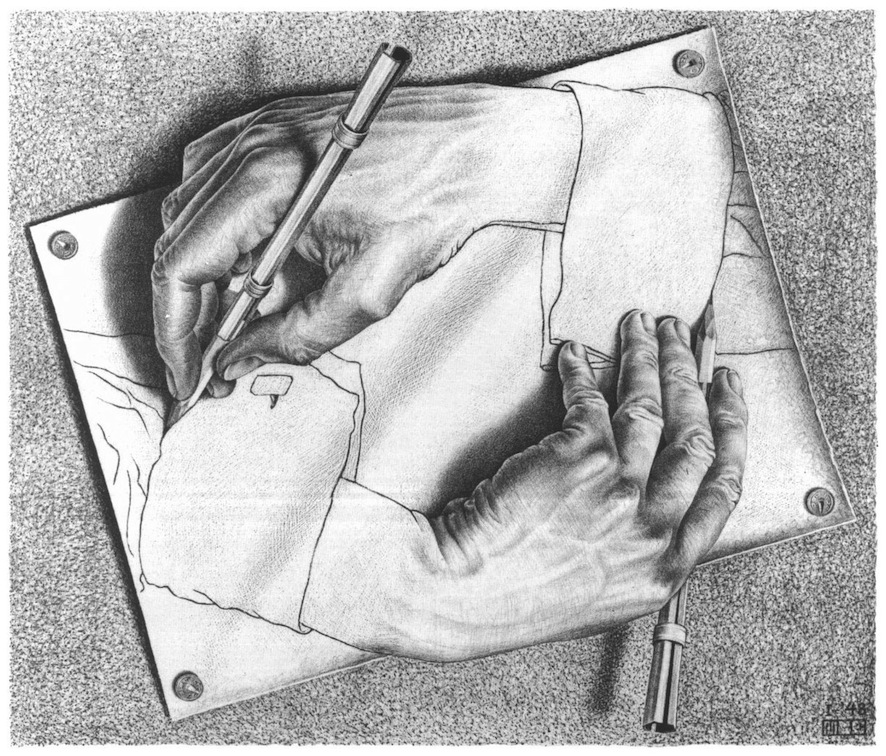
\includegraphics[width=150mm]{cover_escher.jpg}

\thispagestyle{empty}
\cleardoublepage
	
\vspace*{12ex}

\huge{\textbf{\titel}}\\[5ex]
%\Large{\untertitel}\\[10ex]

\large{\textit{\art}}\\
\large{\textit{\fachgebiet}}\\[14ex]

\normalsize
\begin{tabular}{w{5.4cm}p{6cm}}
 penned by: & \quad \autor\\
 mail address: & \quad \mail\\
 matriculation nr.: & \quad \matrikelnummer\\
 area of studies: & \quad \studienbereichA \\
 			& \quad \studienbereichB \\[2ex]
 censor: & \quad \gutachter\\
 second censor: & \quad \zweitgutachter\\
 supervisor: & \quad \betreuer\\[2ex]
 filing date: & \quad \abgabe
\end{tabular}

\tiny \noindent \\[12ex]
\copyright 2012 by \textit{Lukas N.P. Egger}, all Rights Reserved. The cover was created by \textit{Sivan Lutaty}, inspired by the work of \textit{M.C. Escher}.\\
This work is licensed under a Creative Commons Attribution-NonCommercial 3.0 Unported (\href{http://creativecommons.org/licenses/by-nc/3.0/}{CC BY-NC 3.0}).
\begin{figure}[hb]
\centering

\includegraphics[scale=0.75]{creative_commons.png}
\end{figure}








\end{center}
\end{titlepage}

% für Druck Leerseite
\thispagestyle{empty}
\cleardoublepage
	
% Seitennummerierung, vor dem Hauptteil in großen römischen Ziffern 
\pagenumbering{Roman}

% Begin Fußzeilen
\cfoot{- \pagemark \hspace*{0.75ex}-\\}

%Zusammenfassung
\vspace*{1ex}
\section*{Abstract}
\label{abstract}

This thesis focuses on the user-guided simplification of geometric models, i.e. the decimation of in 3D embedded triangle meshes.
Within this area, research spends its attention mostly on deterministic and fully automated algorithms.
The goal of this work however is not to add a new part to the standard ensemble, but instead look into the gains that can be achieved by user interaction combined with non-deterministic approaches.
Thus not only the possibility for artistic control changes, but also the benchmarks for various aspects of the problem, e.g. speed has to be gauged henceforth against the requirements for fluid interactive work.\\
Apart from the obligatory part of the discussion of results there is also a brief historical outline of mesh simplification, a primer to the mathematical skill-set necessary to tackle the emerging phenomena, as well as an outlook on further research questions.\\[1ex]

\section*{Zusammenfassung}
\label{zusammenfassung}

Diese Arbeit widmet sich der nutzergestützten Vereinfachung von geometrischen Modellen.
Innerhalb dieses Bereiches liegt der Fokus gewöhnlich auf deterministischen und vollautomatischen Algorithmen.
Ziel dieser Arbeit ist es aber nicht, dem Kanon an Standardansätzen einen neuen beizufügen, sondern stattdessen die Vorteile von Benutzerinteraktion in Kombination mit nicht-deterministischen Ansätzen zu beleuchten. 
Dadurch verschiebt sich nicht nur die artistischen Kontrollmöglichkeiten, sondern auch der Maßstab in vielen Bereichen, bspw. muss Geschwindigkeit fortan anhand direktem und flüssigen Arbeitens bewertet werden.\\
Neben dem obligatorischen Teil, welcher sich den erarbeiteten Ergebnisse widmet, gibt es auch einen kurzen geschichtlichen Abriss der Entwicklung dieses Spezialgebietes, als auch eine Einführung in die Topologie, welche zur Beschreibung der auftretenden Phänomene benutzt werden kann, sowie einen Ausblick auf weiterführende Fragestellungen. 

\addcontentsline{toc}{chapter}{Abstract \& Zusammenfassung}
% Benutzte Formeln
%\vspace*{1ex}
\section*{Used Notations}
\label{notations}

Definitions of mathematical terms are generally given within paragraphs of text, rather than displayed separately like theorems\footnote{ I follow the style recommendations used by \textit{Allen Hatcher} \citep[cf.][]{Hatcher2002}.}.
\begin{table}[htpb] \medskip
\setlength{\tabcolsep}{5pt}
\renewcommand{\arraystretch}{1.25}
   \label{tab:notations} \caption{Definitions}
\begin{tabular}{ l l }
	$\mathbb{R, Z,}$ etc.: & rationals, integers and so forth.\\
	$\mathbb{R}^{n}$: & $n$-dimensional Euclidean space, in particular $\mathbb{R}^{0} = \mathbb{C}^{0} = \{0\}$.\\
	$\mathcal{S}^{n}$: & the unit sphere in $\mathbb{R}^{n+1}$\\ & i.e. all points of distance: $|d|=1$, from the origin.\\
	$\mathcal{D}^{n}$: & the unit disk or ball in $\mathbb{R}^{n}$\\ & i.e. all points of distance: $|d| \leq 1$, from the origin.\\
	$\partial \mathcal{D}^{n} = \mathcal{S}^{n-1}$: & the boundary of the $n$-disk, respectively $\partial$ the boundary operator.\\
	$\mathrm{e}^{n}$: & an $n$-cell, homeomorphic to the open $n$-disk: $\mathcal{D}^{n} - \partial \mathcal{D}^{n}$,\\ & for instance $e^{0}$ consists of a single point, but $\mathcal{S}^{0} = \partial \mathcal{D}^{1}$ of two.\\
	$\mathcal{M}$: & orientable manifold mesh with $\mathcal{V}$ \& $\mathcal{F}$ the list of vertices \& faces \\ & and $|\mathcal{V}|$ the cardinality respectively $||\mathcal{M}_{A} - \mathcal{M}_{B}||$ the distance.\\
	$\cong, \approx, \simeq$: & isomorphism, homeomorphism and homotopy, \\ & with $\approx \, \Rightarrow \, \simeq$ but not the other way around.\\
	$\mathbb{X}$: & topological space with sets $\mathrm{A}_{i}$.\\
	$\pi_{n}(\mathbb{X})$: & the fundamental group of a topological space,\\ & $\pi_{n}(\mathbb{X}_{1}) = \pi_{n}(\mathbb{X}_{2})$ does not imply $\mathbb{X}_{1} \approx \mathbb{X}_{2}$.\\
	$\equiv$: & congruence relation, i.e. equivalence relation on an algebraic structure.\\
	$\mathrm{K}$: & simplicial complex built from a finite set of simplices: $\{ \sigma^{dim}_{nr} \}$\\ & with an associated filtration: $ \emptyset = \mathrm{K}_{-1} \subset \mathrm{K}_{0} \subset \mathrm{K}_{1} \subset \dots \subset \mathrm{K}_{n} = \mathrm{K}$.\\
\end{tabular}
\end{table}\\
There are also a few notations used in this book that are not completely standard:
The union of a set $\mathrm{A}$ with a family of sets $\mathrm{B}_{i}$, with $i$ ranging over some index set, is written simply as $\mathrm{A} \cup_{i} \mathrm{B}$ rather than something more elaborate such as $\mathrm{A} \cup (\cup_{i} \mathrm{B})$. Other similar operations are treated in the same way.

\addcontentsline{toc}{chapter}{Used Notations \& Symbols}

% Inhaltsverzeichnis
\tableofcontents

% von nun an in normalen arabischen Ziffern
% ohne \clearpage dreht der Befehl durch
\thispagestyle{empty}
\section*{}
\newpage
\thispagestyle{empty}
\section*{}
\newpage % übler Hack
\thispagestyle{empty}
\section*{}
\newpage
\thispagestyle{empty}
\section*{}
\newpage % übler Hack
%\clearpage
\pagenumbering{arabic}

% --------
% Inhalt
\chapter{Introduction}
\label{introduction0}
\vspace{-0.25cm}
\section{The Complexity Conundrum}
\label{introduction1}

\begin{flushright}
\textit{``Reality is 80 million polygons per second''\,\footnote{ There used to be this quipped saying back in the early days of 3D rendering. It was a great catchphrase at the time because during those days, it was an obscene number -- ridiculously beyond the technology of the day. But nowadays, ... , even cheap console systems can crank out that kind of performance. More importantly, today's technology can render that many polygons in realtime with tons more features than was ever available before, such as programmability or multiple passes. And the high-end keeps getting higher. \citep[John Carmack, co-founder of id Software, cited in:][]{Kosak2005}}}\\
-- Alvey Ray Smith \citep[co-founder Pixar, cited in:][p.168]{Rheingold1991}
\end{flushright}

Computer Graphics, much as related fields in Computer Science, has seen an awe-inspiring rate of progress over the last decades.
Yet it seems to be a peculiar fact that advances in Computer Graphics at times appear to be invisible, albeit being often directly translated to prettier pictures and more visceral applications.\\
Normally at this point most people reference the infamous success story of increased computational power, known as \textit{Moore’s Law}\footnote{ The prediction was initially stated in 1965 by Intel co-founder Gordon Moore and held up with physical law-like precision for the last half-century (for the original reference and its context see Appendix \ref{appendix1}).}.
Less widely understood, but even more remarkable is the fact that in most areas, performance gains due to improvements in algorithms have vastly exceeded the performance gains due to increased processor speed\footnote{ It’s difficult to quantify the improvement, though, because it is as much in the realm of quality as of execution time.
In the field of numerical algorithms, however, the improvements can be quantified more straightforwardly.
One example, provided by Prof. Martin Grötschel: A benchmark production planning model solved using linear programming improved by a factor of roughly 43 million between 1991 and 2008.
Of this, a factor of roughly 1,000 was due to increased processor speed, whereas a factor of roughly 43,000 was due to improvements in algorithms \citep[][cf. p.71]{Holdren2010}.}.
When asked about the significant advances over the last 20 years \textit{Ed Catmull} explained how sometimes \textit{``we felt it was at an impossible level''} what they were trying to reach in terms of quality, but now years later \textit{``we have exceeded that level in terms of scene and render complexity -- we have gone beyond impossible''}\,\footnote{ See Appendix \ref{appendix2} for a timeline of important technological advances of RednerMan.} \citep[Edwin „Ed“ Catmull, president of Walt Disney \& Pixar Animation Studios, citet in:][]{Seymour2008}.\\
Despite the industries incredible success, \textit{Catmulls} remark about the complexity as being \textit{“beyond impossible”} appears to contradict the notion of super-exponential technology growth in the field of Computer Graphics.
For instance, rendering times have been constant\footnote{ For Industrial Light \& Magic’s visual effects work on the 1993 film Jurassic Park, typical overnight render times were 4 hours per frame. When the same company worked on the 1997 movie sequel, using both faster computers and more advanced software, frame times were typically an identical 4 hours. Each small speed-up, tends to be used for greater input complexity rather than greater interactivity.\\ While the precise value of the “threshold of pain” for render time varies by institution, this effect has been widely observed. Jim Blinn famously remarked, “All frames take 45 minutes,” hence the effect is known as Blinn’s Law \citep[][cf. Chapter 3]{Enderton2011}.}  for animation films over the last two decades, although algorithms and hardware got so much better during the same time.
If the movie business holds as an example\footnote{ I personally think that animation and special effects driven movies are vibrant examples for the tremendous progress, that the field of Computer Graphics has seen over the last decades. Although I am sure, other interesting references could be made, most of the examples I will give are related to the \textit{VFX-Industry}. For one because I find them to be compelling and vivid, but more so because it is the one field I have personal experience in, due to my internship at \textit{Weta Digital} in 2011.}, it begs the question: How is this possible?
% Bild
\begin{figure}[ht]
\begin{minipage}[b]{0.475\linewidth} \centering
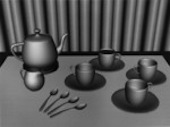
\includegraphics[scale=1.0]{utah_teapot_render.jpg}
\caption{Teapot rendering scene as presented in \textit{Martin Newell's} PhD dissertation, published in 1975 \citep[cf.][]{Torrence2006}.}
\label{fig:utah_teapot_render}
\end{minipage}
\hspace{0.35cm}
\begin{minipage}[b]{0.475\linewidth}
\centering
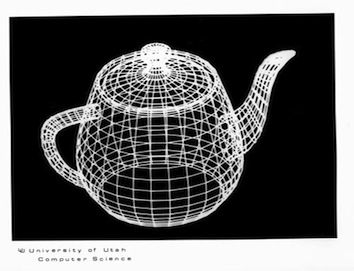
\includegraphics[scale=1.0]{utah_teapot_model.jpg}
\caption{The original wireframe 'Utah Teapot' (28 bicubic Bézier patches, with 16 control points each) \citep[cf.][]{Newell1975a}.}
\label{fig:utah_teapot_model}
\end{minipage}
\end{figure}\\
The answer is ever increasing complexity!
Increasing complexity regarding: Lighting techniques, phenomena that are simulated, and many other domains but most importantly the increased complexity of the assets used for rendering.
Every studio struggles with heavier and heavier assets, i.e. the sheer size in geometry information used for models:
\textit{``Our typical rendered scenes [for work on Marvels 'The Avengers' (2012)] contain over 140 million triangles across thousands of objects though we have pushed over 1 billion polygons''} \citep[Votch Levi, CTO Whiskytree, cited in:][]{Seymour2012}.

To illustrate this hasty evolution, one simply has to look at the stark contrast between the models used for the top-of-the-line renderings of 1975, namely the 'Teapot scene' and a scene from the 2009 movie 'UP', as shown in the pictures \ref{fig:utah_teapot_model} and \ref{fig:micropolys}.
Whereas all the information needed to describe the models in the 'Teapot scene' could be fit on one page of paper\footnote{  For more information about the original Teapot renderings and a facsimile of the model description, see Appendix \ref{appendix3}.}, the models currently in production regularly max out in the domain of several giga-bytes of raw data per asset.
% Bild
\begin{figure}[ht]
\begin{minipage}[b]{0.475\linewidth} \centering

\includegraphics[scale=0.72]{screenshot_up.jpg}
\caption{Example of highly detailed surface -- the houndstooth pattern of the jacket is genuine geometric data {[}Credit: Pixar 2009{]}.}
\label{fig:screenshot_up}
\end{minipage}
\hspace{0.35cm}
\begin{minipage}[b]{0.475\linewidth}
\centering
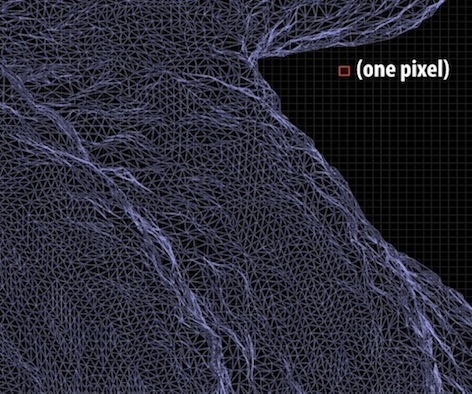
\includegraphics[scale=0.72]{micropolys.jpg}
\caption{To leave no evidence that surfaces are discretely approximated, film models consist of micropolygons, about a pixel in area \citep[][p.7]{Fatahalian2011}.}
\label{fig:micropolys}
\end{minipage}
\end{figure}

\section{The Case for Highly Detailed Geometry}
\label{introduction2}

Regardless of the factual costs and critical handling issues when working with this kind of scope and complexity, the trend appears to be unbroken\footnote{ 
The importance of highly accurate modeled surfaces has always been an crucial factor for (offline) rendering systems \citep[cf.][]{Cook1987}, but especially with tent-pole movie productions, this paradigm seems to know only one direction -- that is -- bigger meshes: ``the complexity continues to scale on each project we do, the amount we need to render continues to multiply...'' -- 'Avatar' (2009), was the first movie project that exceed 2 petabyte of storage data \citep[Martin Hill, head of shading at Weta Digital, cited in:][]{NVidia2009}.}.
The reason for this is, that in order to render richly detailed and artifact-free scenes, complex models are inevitable.
Over the time there have been numerous ingenious strategies to cut corners, such as precomputed static illumination, bump-, normal- and occlusion-mapping, etc. to compensate for the lack of geometric detail, especially in interactive applications \citep[cf.][]{Akenine-Moller2008}.
These techniques have comparatively low rendering cost and are used effectively in games.
However, they are prone to artifacts.
%Bild
\begin{figure}[ht]
\centering
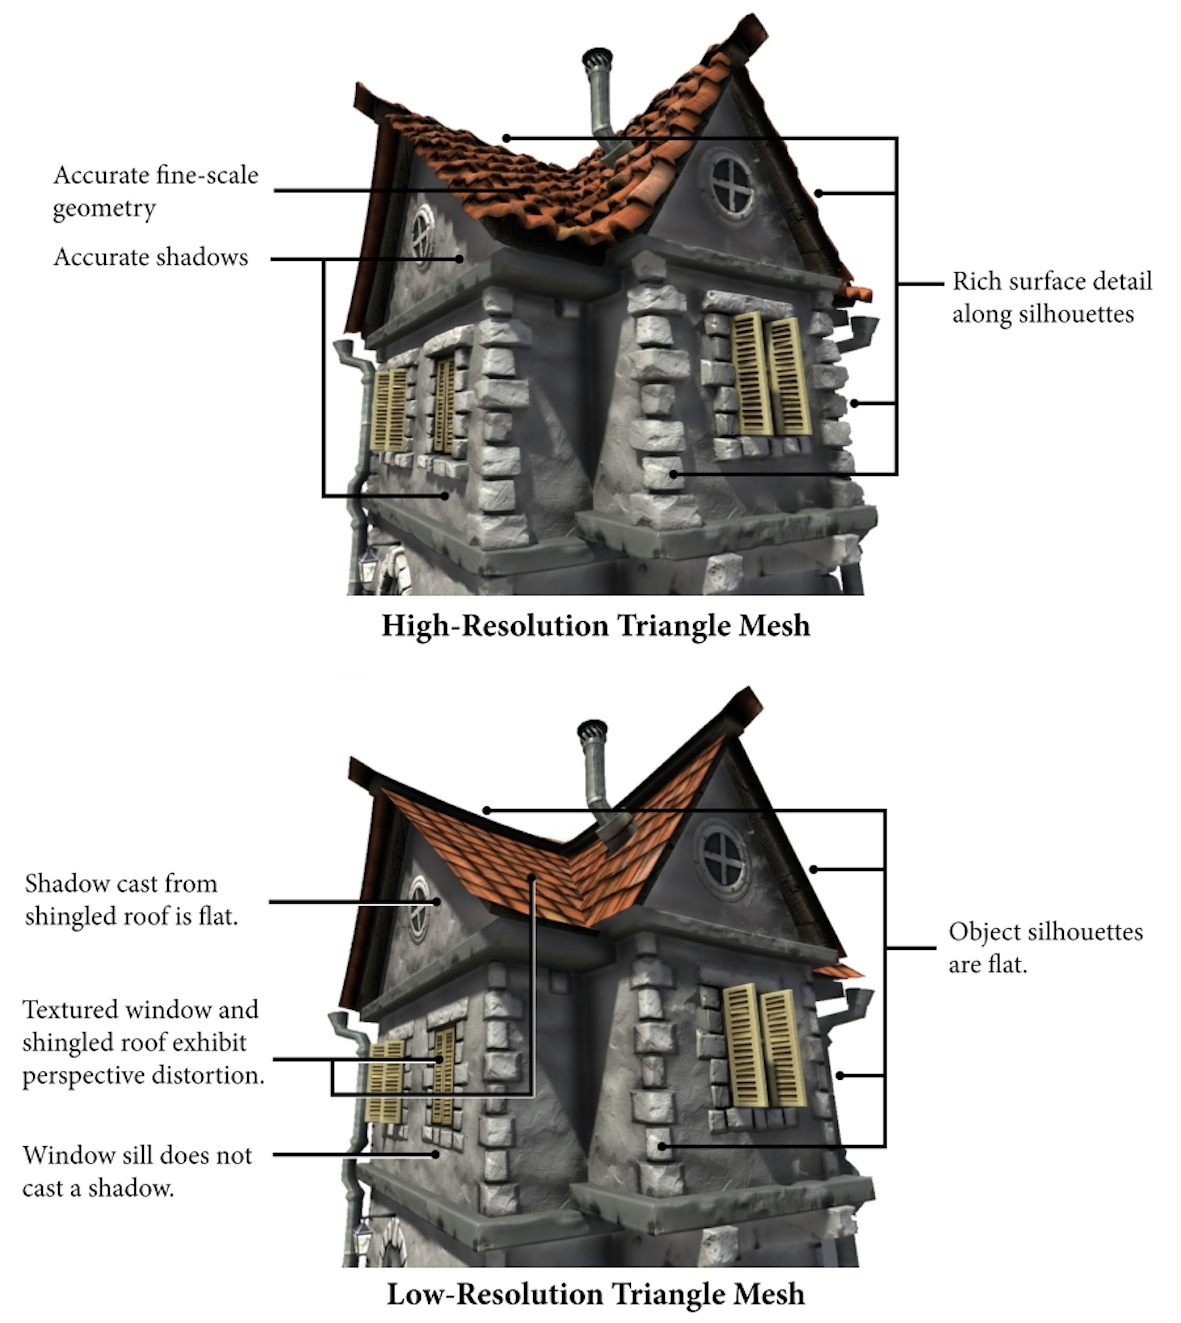
\includegraphics[width=0.95\textwidth]{lowpoly_vs_highpoly.jpg}
\caption{Renderings of a stone house using a high-resolution (top) and low-resolution (bottom) triangle mesh (house image by Unigine Engine).}
\label{fig:lowpoly_vs_highpoly}
\end{figure}\\
The stone house pictured in \ref{fig:lowpoly_vs_highpoly} features many complex surfaces like bumpy cornerstones and curved red roof-tiles.
Accurate shadows (self-shadowing) are cast and self occlusion can be seen.
These details can be rendered because the house is represented using a high-resolution triangle mesh.
The lower image, uses the same texturing and soft shadowing techniques, but with scene geometry represented using a low resolution triangle mesh.
The model holds up quite well, but unfortunately, the illusion breaks down eventually.
Especially along the house’s silhouettes, artifacts are spotted easily.
Shadows are rendered but on close examination they also give away the flat nature of the low resolution stand-in.
Similarly, the roof tiles and windows on the left side of the image appear distorted.
These artifacts become even more noticeable when objects move \citep[cf.][p.2-4]{Fatahalian2011}.\\
Undoubtedly the industry will continue to push polygon counts for the next years, on its pursuit for visual brilliance and high fidelity\footnote{ During my internship I personally asked a modeler, at what point they would normally stop adding geometric detail? He noted that everyones biggest fear is to get ones' work rejected because it does not hold up to a supervisors expectations. So what they will do is to work until their tools -- their computers and software -- give in and make it unbearable to work any further.}.
Together with the scaling of complexity also scales the need for tools that facilitate the work with the created data.
Whether you believe that the artist or the tools at his disposal are the principal or the agent, it is for sure, that without robust and capable techniques no creation would be possible.
And at the forefront of fundamental techniques for geometry processing is mesh simplification.

\section{Mesh decimation}
\label{introduction3}

Mesh decimation or simplification is both, a very current, and a very old idea in computer graphics.
As early as 1976 \textit{James Clark} described the benefits of representing objects within a scene at several resolutions \citep[cf.][]{Clark1976}.\\
Dozens and dozens of simplification algorithms have been developed in the meantime.
Even a number of excellent surveys reviewing the field of polygonal simplification have been published\footnote{ For example, Cignoni et al. supplied comparative performance statistics for over 30 different decimation strategies \citep[cf.][]{Cignoni1998, Heckbert1997}.}.
Yet, no algorithm today excels at simplifying all models equally good.
Some approaches best suit curved organic forms, while others work best at preserving hard planar objects with sharp corners, flat faces, and regular curves.
This is probably due to the fact that, we still have limited understanding about what really determines perceptual fidelity.
We do have a good understand of geometric and volumetric fidelity but as it turns out, the supposedly easy question:  Does the simplification look like the original?
Is hard to answer \citep[][cf. p.25]{Luebke2001}.\\
At this point it seems that the research community tends to be of the opinion, that until the question of perceptual metrics is solved, the research area of mesh simplification is in a state of arrested development\footnote{ Only few ameliorations have been proposed, mostly at the cost of near-to prohibitively expense execution times, like Cohen’s ``Appearance-Preserving Simplification'' \citep[cf.][]{Cohen1998} and Lindstrom’s ``Image-Driven Simplification'' \citep[cf.][]{Lindstrom2000} -- both of which aiming at per-pixel comparisons of multiple rendered views as ``weights'' or upper bounds for the priority queue of an incremental decimation process.\\For an comprehensive discussion about the difficulties faced when trying to define perceptually salient descriptors see ``Perceptual metrics for static and dynamic triangle meshes'' \citep[cf.][]{Corsini2012}, respectively ``Perceptually Driven Simplification for Interactive Rendering'' for further information on psychophysical models of visual perception \citep[][]{Luebke2001a}.}. 
As much as I agree that it would be fantastic to get a sound scientific grasp of human perception, I reject the notion that exciting research topics aren't to be found.\\
At the beginning of most journal papers concerning mesh decimation, the same emblematic application examples are listed: meshes generated by marching-cubes, CAD/CAM models, oversampled 3D scan data, etc. -- but with the advent of image based automatic geometry capture techniques and their impressive results \citep[cf.][]{Pollefeys2004,Snavely2008}, arguably the scope of the field has changed\footnote{ Another branch of research that will affect the evolution of geometry processing tools in a profound way, is 3D printing and rapid prototyping -- if only for the scale, once with wide-spread adopted \citep[cf.][]{Vilbrandt2008,Bickel2010}.}.
Not only is there a demand for highly detailed meshes but also a plethora of source material to work with.
%Bild
\begin{figure}[ht]
\centering
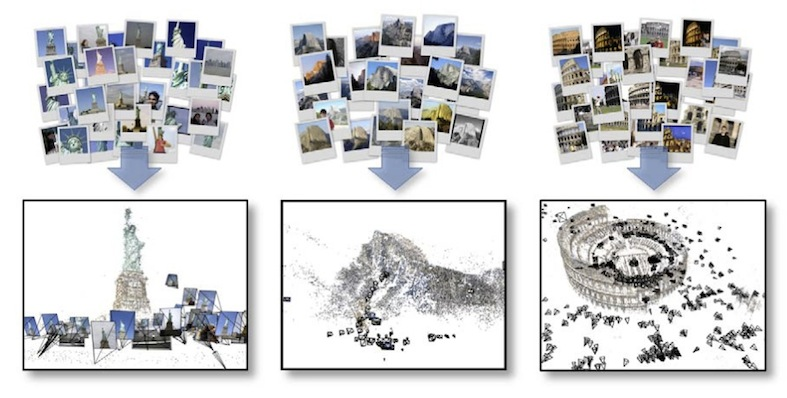
\includegraphics[width=0.95\textwidth]{image_synthesis.jpg}
\caption{3D mesh reconstructions from Internet photo collections, that typically can have dozens of millions of triangles \citep[][p.6]{Snavely2008}.}
\label{fig:image_synthesis}
\end{figure}\\
Still, the research community does not emphasis on mesh decimation as of lately.
One of the reason for this, is the set of expectations that govern academic zeitgeist.
For example, ``good'' solutions are considered to be solutions that have been completely automated with little or none required input from the user.
However there is much to be gained and researched, once the user is seen as integral part of the process.
\begin{quote} \textit{``Decimation of generated models, often reduces the precision ... and while the generated meshes may have the correct level of detail, it is not represented in a structured form, usable in subsequent stages ... In many cases it would be more useful to rely on user input to generate a simplified, yet structured mesh that can be further manipulated.''} \citep[p.195]{Sylwan2011} \end{quote}
Bringing together the arguments of the last pages, the important question to ask now is, what kind of requirements should a modern mesh decimation algorithm focus on?

\section{Design Principles \& Workflow Regimes}
\label{introduction4}

The first step in deciding upon the design features of an application that simplifies meshes, is to acknowledge that there will never be one perfect solution to fit all possible scenarios.
Not only because there are always trade offs to be made in engineering, but because there are conflicts of objectives that oppose each other diametrically.
For instance, it is not possible to ensure quasi 'Delaunay-Triangulation' in order to cater for the needs of an finite elements simulation and at the same time aggressively reduce the vertex count without loosing geometric detail\footnote{ Arguably there will be always just two out of the following three: good triangle shape / high decimation / fidelity -- and many other examples for goal conflicts can be found.}.\\
The route that shows more promise instead, is to put an emphasis on a few selected, crucial aspects.
Thus our work focuses on two major principles that were decided beforehand:
\begin{itemize}
    \item Full topology control during the decimation process.
    \item Artistic freedom by the means of user-guidance.
\end{itemize}
As for the first aspect -- topology control -- most algorithms do ensure the preservation of the topological genus of a given model\footnote{ With the notably exception of the class of vertex clustering algorithms, that by design, are agnostic to topological changes \citep[cf. the original paper by][]{Rossignac1993}.}, but only rarely are topological features by themselves a criteria for decimation.
Accounting for this poses some interesting research questions that have not yet been yet answered satisfactorily.
It is also the more theoretical and abstract part of the thesis.\\
The second aspect -- artistic freedom, i.e. user-guidance -- has some further ramifications that need to be discussed.
Unquestionably it appears to be a good thing to give additional control to the user.
Not only can the hard problem of perceptual fidelity be handed over to the one instance best suited for the decision, but also there can be direct feedback incorporated to ensure the ideal outcome.
\begin{quote} \textit{``Often researchers are biased towards a fully automated solution or assume the user interaction needs to be targeted to a novice user.''} \citep[p.195]{Sylwan2011} \end{quote}
%Bild
\begin{floatingfigure}[r]{0.40\textwidth}
\centering
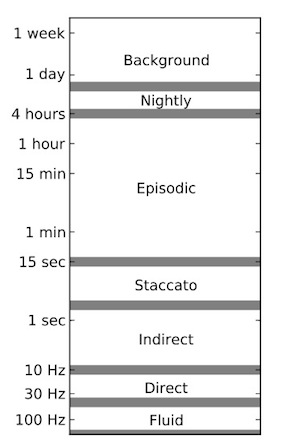
\includegraphics[width=0.33\textwidth]{workflow_regimes.jpg}
\caption{Response time to user input vs. workflow.}
\label{fig:workflow_regimes}
\end{floatingfigure}
Just adopting some measure of control not automatically yields better results. 
In order to leverage the outlined advantages, the entire system has to meet the needs of direct user interaction.
There is a balance between interaction and computation.\\
If a process gives perfectly accurate results automatically, it is a candidate to run unsupervised in an multiply hour offline scenario.
Whereas an algorithm that requires artist intervention, must run relatively quickly so artists get immediate feedback and iterate on it \citep[cf.][p.20]{Hillman2010}.
This sounds like an obvious observation, but research has shown, that missing certain levels of interactivity, ultimately decides upon how a tool is viewed as a whole and thereby determines the success and adoption rate of this technology \citep[cf.][]{Enderton2011}.
\begin{quote} \textit{``A workflow regime is defined as a range of system response times in which the artist’s relationship to the task is qualitatively similar ... technology is much more likely to succeed when it brings an artist’s workflow into a new regime ... we feel physically connected, albeit indirectly. This connection is critical for focused and rapid task achievement.''} \citep[p.2]{Enderton2011} \end{quote}

In summary what we want is a very fast, hence smoothly interacting application that gives good results but invites the user to tweak any aspect of it until the best possible outcome is reached.
This is in short is what this thesis' goal is!\\

\section{The Outline of this Thesis}
\label{introduction5}

The introduction started with a general observations on trends:
Complexity from the point of view of Computer Graphics has increased dramatically over the last decades and is still on the rise.
This is also especially true for geometric complexity, since even the best short-cuts can leave one with undesired artifacts. 
With models getting more and more detailed, the need for good tools that can simplify meshes likewise increases. 
But instead of adding a new algorithm to the standard repertoire, we propose to focus on adopting techniques for user guidance and topology control.
After this widely argument for our motivation, the rest of the thesis is structure pretty much straightforward.

The next section, chapter \ref{simplification0}, will very briefly discuss the historical development of the field of mesh decimation.
Not so much in order to give an exact overall account, but rather to give an overview of the principle techniques and the ideas behind them.\\ 
This is followed by chapter \ref{math0}, that functions as a primer for certain mathematical concepts which are crucial for the understanding of topology.
Topology control is one of the key contributions of our work and although the comprehension of the involved mathematics is important, it is not a mandatory prerequisite for the remaining text.\\
Chapter \ref{topstoc0} finally details and discusses the contribution of our work.\\
The last part, chapter \ref{conclusion0}, tries to summarize the work and to give an outlook on further research topics.

\chapter{The Concept and History of Mesh Simplification}
\label{simplification0}

\section{Problem Statement}
\label{simplification1}

\begin{flushright}
\textit{``The essence of mathematics is ... to make complicated things simple.''}\\
-- Stan Gudder
\end{flushright}

Before considering any concrete approaches or talking about historical developments of mesh simplification, we want to give a formal definition of the problem.
For a given mesh $\mathcal{M} = \{\mathcal{V},\mathcal{F}\}$ where $\mathcal{V}$ is the list of vertices and $\mathcal{F}$ the list of faces indexed over $\mathcal{V}$, we search for $\mathcal{M'=\{\mathcal{V'},\mathcal{F'}\} \subset M}$ so that either:
$|\mathcal{V'}|<|\mathcal{V}| \text{ with } |\mathcal{V'}| \in [n_{min}, n_{max}] \text{, and } \|\mathcal{M}-\mathcal{M'}\| \text{ is minimal -- the so called budget-based approach, or } \|\mathcal{M}-\mathcal{M'}\| < \epsilon \text{ and } |\mathcal{V'}| $ is minimal -- a fidelity-based simplification, led by some measure of difference $\epsilon$.
Most of the time this is done together with further constraints like globally enforced fairness criteria\footnote{ What is typically used, are geometrical analogies of the first and second fundamental form of differential geometry, transferred to the discrete setting of triangle meshes. For example \citep[cf.][]{Schroder2003}:
\begin{itemize}
{\setlength\itemindent{14pt} \item[Order 0: ] distance vertex and plane, parametric or geometric distance}
{\setlength\itemindent{14pt} \item[Order 1: ] local distortion, triangle shape or inradius}
{\setlength\itemindent{14pt} \item[Order 2: ] local or mean curvature, sum dihedral angles}
{\setlength\itemindent{14pt} \item[No order: ] e.g. valence balance or scalar attributes that can account for other arbitrary restrictions}
\end{itemize}} to evaluate the quality of
the mesh $\mathcal{M'}$: \textit{``the use of a fairness oracle turns the plain downhill decision of the greedy algorithm into an 'educated guess' ''} \citep[][p.46]{Kobbelt1998}.\\
This means that mesh simplification describes a class of algorithms that transform a given polygonal mesh into another with fewer faces, edges and vertices.
% $n=|\mathcal{V'}|$\footnote{ \textbf{Lemma:} For any manifold mesh it follows that $|\mathcal{V}|>|\mathcal{V'}|$ implies $|\mathcal{F}|>|\mathcal{F'}|$, respectively less edges.}
Thus a mesh simplification scheme can be viewed as a decomposition operator to obtain a low frequency component $\mathcal{M'}$ and a high frequency component, i.e. the difference ($\mathcal{M} - \mathcal{M'}$).
The decimation process is usually aimed at a specific target size and controlled by a set of user-defined quality measures that aim to preserve specific properties and salient features of the original mesh as much as possible \citep[][cf. pp.9-10]{Shene2005}.

%\newpage
%\vspace*{1ex}
\section{Chronology of Simplification Designs}
\label{simplification2}

The idea to use different resolutions of the same model can be traced back, as far as 1976 \citep[cf.][]{Clark1976}\footnote{ Clark's 
paper ``Hierarchical Geometric Models for Visible Surface Algorithms'' also described hierarchical scene graph structures and by todays standards mundane techniques, such as view-frustum culling and out-of-core simplification. Nevertheless it is interesting to read for its value as a foundational paper of Computer Graphics.} but at the time all low-resolution proxies of models were created manually.
Only in the early 1990s the first algorithms to automate this process appeared.
The new field instantly spiked interest in the research community and a flurry of papers were published in the following years.
Some of those first algorithms, such as vertex decimation \citep[][]{Schroeder1992} and vertex clustering \citep[][]{Rossignac1993}, remain viable and useful solutions until today.\\
Today there is an abundance of designs for algorithms to choose from, literally hundreds of different solutions for mesh decimation.
Therefore we can not and do not want to discuss every single algorithm ever conceived, but instead we give a chronology of very influential works with a short description of the idea behind it.
Thereby showing the numerous ways in which decimation can be done.
For a more detailed discussion of the history of the field, see \citep[][cf. p.4 ff.]{Diaz-Goano1998} and \citep[][cf. p.8 ff.]{Luebke2002}.
Almost every paper today can be referenced to one of the following works or rather these designs:
%Liste
\begin{itemize}
    \item Selectively removing vertices \citep[cf.][]{Schroeder1992}.\\
The algorithm makes multiple passes over the set of vertices of the triangle mesh and removes vertices according to predefined criteria. As a result of a removal a hole is created which a triangulation process then fills\footnote{ The number of ways to triangulate a regular polygon with $n+2$ sides, is given by the Catalan numbers. One can think of choosing from among these possible ways as a discrete optimization problem:\\
$C_{n} = \frac{1}{n+1}{2n \choose n} = \frac{(2n)!}{(n+1)!\,n!} = \prod \limits_{k=2}^{n}\frac{n+k}{k} \text{ for } n \in \mathbb{N}$} (also see figure \ref{fig:dec_schroeder}).
%Bild
\begin{figure}[hbt]
\centering
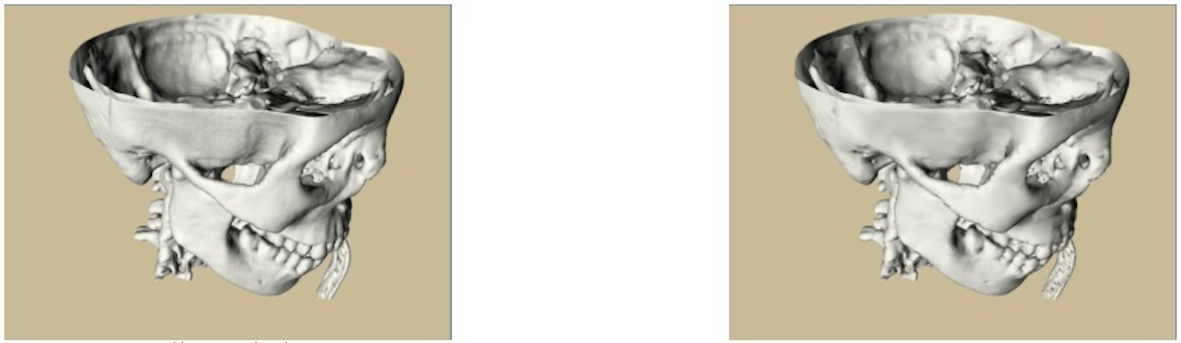
\includegraphics[width=0.85\textwidth]{dec_schroeder.jpg}
\caption{Example from the original paper, left full resolution (569k triangles) and right the 90\% decimated version (142k triangles) \citep[][p.68]{Schroeder1992}.}
\label{fig:dec_schroeder}
\end{figure} 

    \item Redistributing vertices over a surface \citep[cf.][]{Turk1992}.\\
The idea is to reduce the number of polygons by adding new points on the surface of the model, connecting these new vertices into triangles forming a mutual tessellation. Thus creating an intermediate polygonal surface that incorporates both the old vertices and the newly placed ones and then deleting the old vertices, i.e. re-tiling the surface. In order to maintain accurately the features of the surface, the point distribution is modified so that more new vertices are placed in regions of higher curvature (also see figure \ref{fig:dec_turk}).
%Bild
\begin{figure}[ht]
\centering
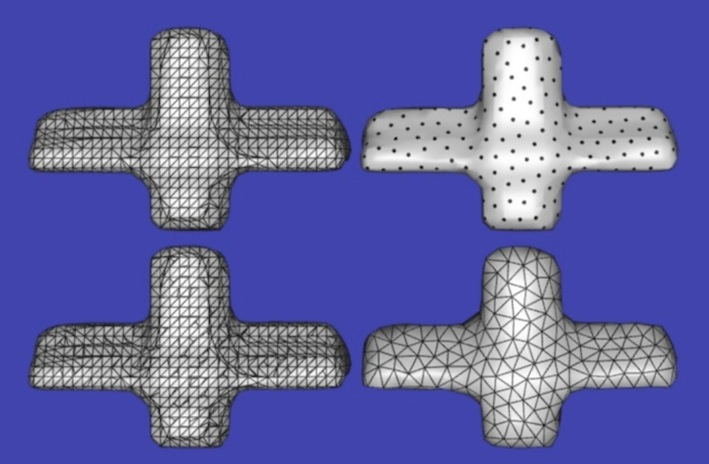
\includegraphics[width=0.50\textwidth]{dec_turk.jpg}
\caption{Re-tiling of a radiation iso-dose surface. Upper left: Original surface. Upper right: Candidate vertices after point-repulsion. Lower left: Mutual tessellation. Lower right: Final tessellation \citep[][p.58]{Turk1992}.}
\label{fig:dec_turk}
\end{figure} 

    \item Clustering vertices \citep[cf.][]{Rossignac1993}.\\
Is done by merging vertices based on their spatial proximity. All vertices within each cell of the subdivided 3D are collapsed into a single representative vertex for the voxel. Hence the resolution of the grid determines the level of detail achieved.
%Bild
\begin{figure}[ht]
\centering
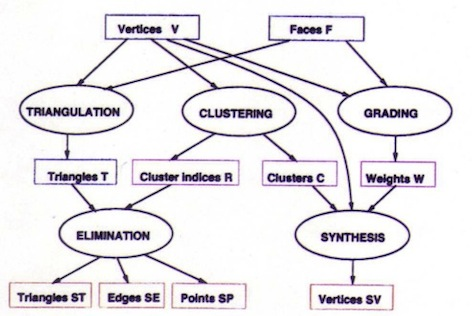
\includegraphics[width=0.60\textwidth]{dec_rossignac.jpg}
\caption{Overview of the simplification process \citep[][p.458]{Rossignac1993}.}
\label{fig:dec_rossignac}
\end{figure}
The algorithm is very robust as it can handle degenerated models, but it is sensitive to the orientation of the clustering grid. It can be implemented quite efficiently. Unfortunately topology is not preserved, and it is very hard to give guaranteed explicit error bounds (also see figure \ref{fig:dec_rossignac}).

    \item Merging nearly coplanar polygons \citep[cf.][]{Hinker1993}.\\
This method obtains impressive reductions for large models with nearly flat surfaces. It identifying coplanar or nearly coplanar polygons, merging them together into a larger complex polygon and finally re-triangulating them into fewer polygons than the original description. However, this approach offers only small gains
for surfaces of high curvature (also see figure \ref{fig:dec_hinker}).
%Bild
\begin{figure}[ht]
\centering
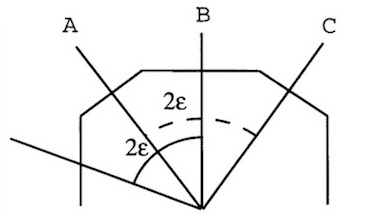
\includegraphics[width=0.30\textwidth]{dec_hinker.jpg}
\caption{
$2\epsilon$ is the user specified angle describing the maximum angular difference between coplanar sets selected to be merged \citep[][p.192]{Hinker1993}.}
\label{fig:dec_hinker}
\end{figure}

    \item Removing polygons in order of curvature \citep[cf.][]{Hamann1994}.\\
Given a surface triangulation, each triangle is weighted according to the principal curvature at its vertices.
These curvature values are pre-computed based on a parametric representation of the surface.
A triangle is associated with a surface region of low curvature if the sum of the absolute curvatures at its vertices is low.
The lower the curvature value at the vertices of a triangle the lower its weight.
The triangle with lowest weight is removed.
The region affected by the removal is re-triangulated and new weights are computed for all affected triangles (also see figure \ref{fig:dec_hamann}).
%Bild
\begin{figure}[ht]
\centering
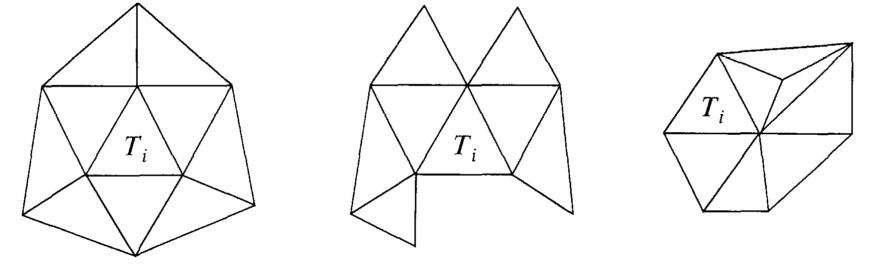
\includegraphics[width=0.70\textwidth]{dec_hamann.jpg}
\caption{The different cases for a triangle platelet $P_{i}$, i.e. the data stencil in the surface triangulation affected by the removal of triangle $T_{i}$ --  platelets with cyclic, disconnected and connected corona \citep[][p.200]{Hamann1994}.}
\label{fig:dec_hamann}
\end{figure}

    \item Using Wavelet theory \citep[cf.][]{Eck1995}.\\
A mesh is converted into a sample mesh together with a sequence of local correction terms, i.e. wavelet coefficients that capture the detail present in the model at various resolutions. The algorithm uses enough wavelet coefficients to meet a user specified error
bound. An important contribution of this method is that it overcomes subdivision connectivity restrictions. It constructs a continuous parametrization of an arbitrary mesh over a simple domain mesh, thus all arbitrary meshes can be converted to multiresolution form (also see figure \ref{fig:dec_eck}).
%Bild
\begin{figure}[ht]
\centering
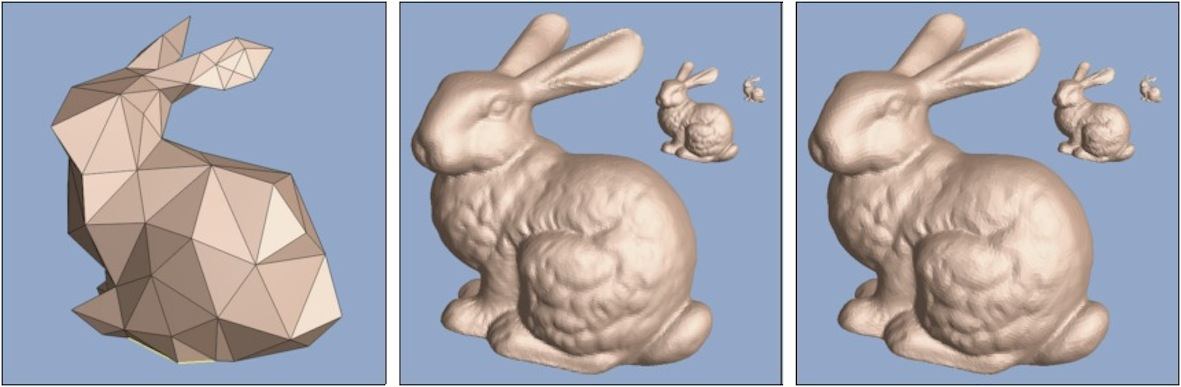
\includegraphics[width=0.80\textwidth]{dec_eck.jpg}
\caption{Left: Base mesh (162 triangles). Middle: Original mesh (69,437 triangles). LOD using multiresolution approximation \citep[][p.181]{Eck1995}.}
\label{fig:dec_eck}
\end{figure}

    \item Minimizing an energy function \citep[cf.][]{Hoppe1996}.\\
Hoppe presents a framework, called 'Progressive Meshes', which consist of a base mesh created by a sequence of edge collapses and vertex splits together with a sequence of detailed records that indicate how to incrementally refine the base mesh exactly back to the original mesh.
%Bild
\begin{figure}[ht]
\centering
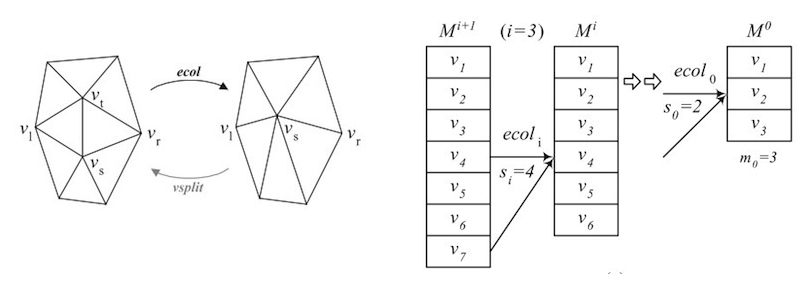
\includegraphics[width=0.90\textwidth]{dec_hoppe.jpg}
\caption{Original illustration of the edge collapse transformation respectively the vertex split and the resulting vertex correspondences \citep[][p.100]{Hoppe1996}.}
\label{fig:dec_hoppe}
\end{figure}
The sequence of collapses during a simplification is determined explicitly as an energy function to be minimized.
All edges to be collapsed are evaluated according to the energy function and sorted in a priority queue.
'Progressive Meshes' also introduced a very efficient data structure that can be used to represent a triangle mesh at multiple levels of detail, i.e. progressive refinement (also see figure \ref{fig:dec_hoppe}).
This techniques has been widely used for view-dependent simplifications, as well as progressive transmissions \citep[cf.][]{Bajaj1999}.

    \item Using bounding surfaces \citep[cf.][]{Cohen1996}.\\
A proposed method called 'Simplification envelopes'.
The approach guarantees an error bound so that all points of an approximation are within a user-specifiable distance from the original model, also it enforces global and local topology preservation.
Simplification envelopes of a surface consists of two offset surfaces.
The outer and inner envelope are generated by displacing each vertex of the original mesh along its normal by a defined distance $\pm\epsilon$, which then guides the process.
A strong suit of this method is that it can gracefully deal with sharp edges (also see figure \ref{fig:dec_cohen}).
%Bild
\begin{figure}[ht]
\centering
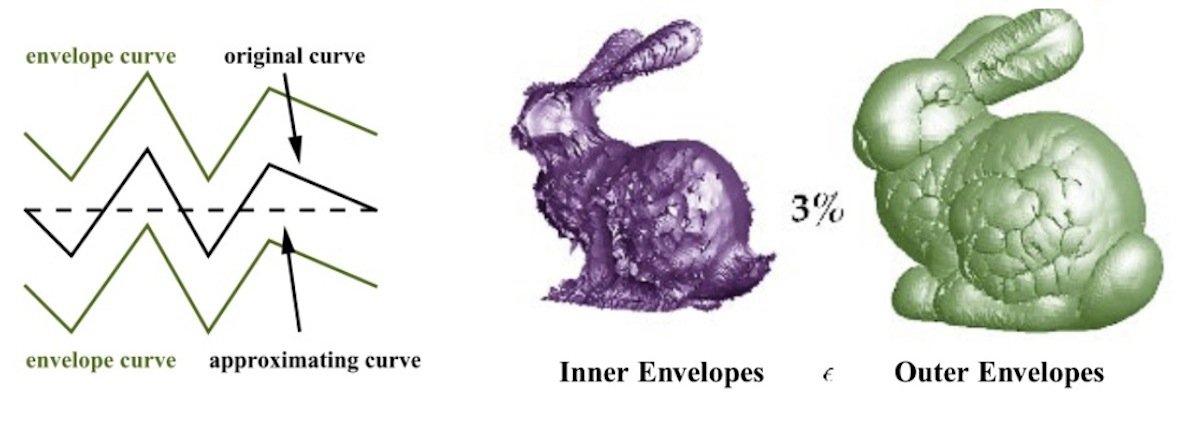
\includegraphics[width=0.80\textwidth]{dec_cohen.jpg}
\caption{Approximation with inner \& outer envelopes \citep[][pp.123-124]{Cohen1996}.}
\label{fig:dec_cohen}
\end{figure}

    \item Quadric Error Metrics \citep[cf.][]{Garland1997}.\\
The algorithm uses iterative contractions of vertex pairs to simplify models and maintains surface error approximations using quadric matrices.
By contracting arbitrary vertex pairs and not just edges, the algorithm can change the topology of the mesh and does not need a manifold mesh to begin with.
As the algorithm proceeds, a geometric error approximation is maintained at each vertex $\mathbf{v}$ of the decimated model: $\Delta(\mathbf{v})= \mathbf{v}^{T}\mathbf{Q}\mathbf{v}$, for a given contraction $(\mathbf{v_{1}},\mathbf{v_{2}}) \rightarrow \mathbf{v_{12}}$ the new matrix $\mathbf{Q_{12}}$ can be easily derived by simply adding $\mathbf{Q}_{1} + \mathbf{Q}_{2} = \mathbf{Q_{12}}$.
Simplification with quadric error metrics possesses much of the generality of vertex clustering as well as the quality and control of iterative contraction algorithms.
The only major downside is its relative slowness compared to vertex clustering (also see figure \ref{fig:dec_garland}).
%Bild
\begin{figure}[ht]
\centering
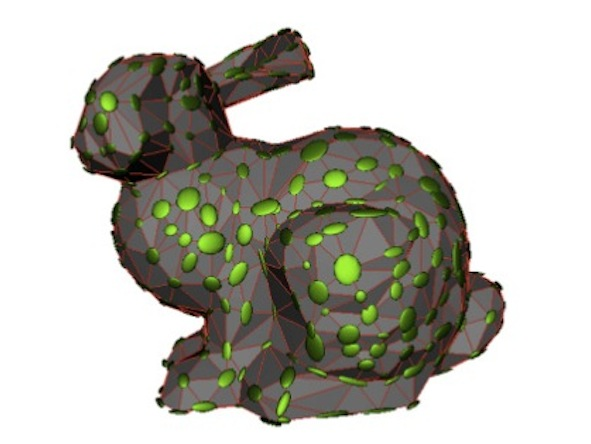
\includegraphics[width=0.35\textwidth]{dec_garland.jpg}
\caption{98,5\% decimation of the stanford bunny. The error ellipsoids for each vertex are shown in green \citep[][p.215]{Garland1997}.}
\label{fig:dec_garland}
\end{figure}

    \item Vertex placement for collapsed edges \citep[cf.][]{Lindstrom1998}.\\
Using edge collapse as the method for simplifying, edges are incrementally replaced with a single vertex.
The new vertex is placed so it preserves the location and shape, and does not require a retriangulation.
The decision of how to position and order the edges builds upon volume and surface information.
Since these conditions do not fully determine the decimation process, an optimization stage is added.
Per triangle volume and area differences are used to create the priority queue (also see figure \ref{fig:dec_lindstrom}).
%Bild
\begin{figure}[ht]
\centering
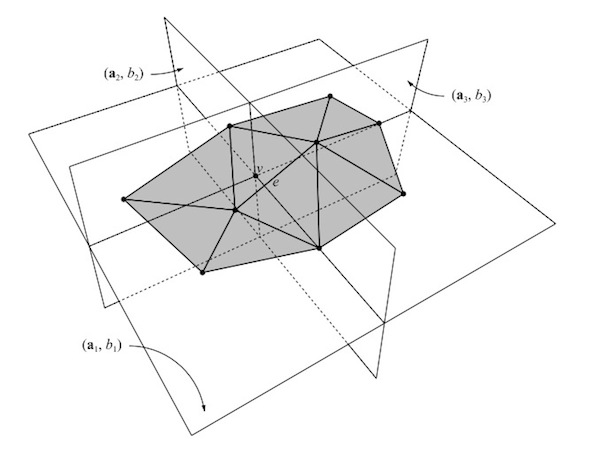
\includegraphics[width=0.45\textwidth]{dec_lindstrom.jpg}
\caption{The optimal vertex position $v$ expressed as the intersection of three planes that ensure volume preservation \citep[][p.284]{Lindstrom1998}.}
\label{fig:dec_lindstrom}
\end{figure}

    \item User-assistance for mesh simplifiaction \citep[cf.][]{Cignoni1998a}.\\
The first system that takes advantage of users-guidance for simplification.
``Zeta: A Resolution Modeling System'', takes a precomputed sequence of simplifications as input, and utilizes an layer of abstraction to work with different local mesh reduction schemes.
Especially noteworthy is that the paper explicitly mentions response times and the role of interactivity (also see figure \ref{fig:dec_cignoni}).
%Bild
\begin{figure}[ht]
\centering
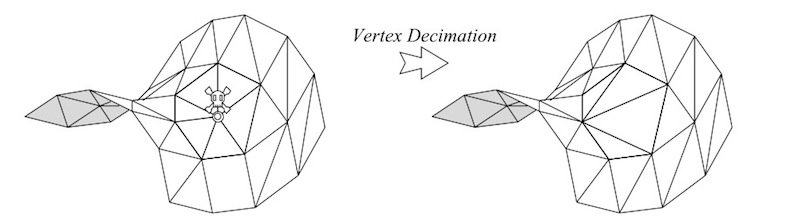
\includegraphics[width=0.65\textwidth]{dec_cignoni.jpg}
\caption{Explicit deletion of a vertex on the mesh \citep[][p.312]{Cignoni1998a}.}
\label{fig:dec_cignoni}
\end{figure}

    \item Using image compression for geometry \citep[cf.][]{Gu2002}.\\
Most of the time surface geometry is modeled with irregular triangle meshes, i.e. not constant valency. In their paper, the authors devise a method to remesh an arbitrary surface onto a completely regular structure they call a geometry image, by this enabling them to represent geometry as a simple 2D array of quantized points. Surface signals like normals and colors are stored in similar 2D arrays using the same implicit surface parametrization. To create this geometry image, the mesh is cut along a network of edge paths, and the resulting single chart is parametrized onto a square\footnote{ More precisely the geometry is mapped onto a torus, since it is the only 3D manifold that can be a completely regular quad mesh and accordingly a regular triangle mesh with valence 6. With two cuts the torus then is equivalent to a 2D array (for a proof of this statement see Appendix \ref{appendix4}).}. The ingenious twist is, that in this form geometry images can be encoded using traditional lossy image compression algorithms, such as JPEG.
A compelling example of how lifting one problem into another domain can lead to unexpected connections and new ideas (also see figure \ref{fig:dec_gu}).
%Bild
\begin{figure}[ht]
\centering
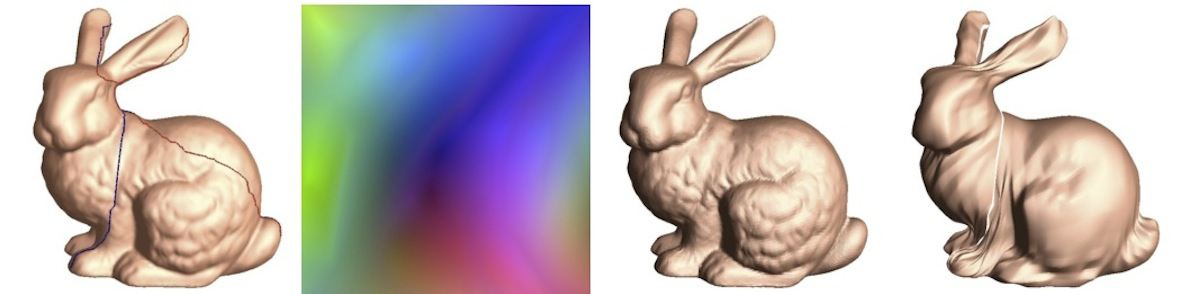
\includegraphics[width=0.9\textwidth]{dec_gu.jpg}
\caption{Left: Original mesh and its geometry image. Right: Reconstruction of the original and a 1,5kB compressed version mesh \citep[][p.356]{Gu2002}.}
\label{fig:dec_gu}
\end{figure}
\end{itemize}
This section can not give an exhaustive nor overall account of mesh simplification, but hopefully by example it illustrated the richness of the solutions and the progress already made.
The next section will try to bring together the various ideas presented here in order to give a general frame of reference, that is to say principles for taxonomies.

\newpage	
\section{Taxonomies}
\label{simplification3}

Besides listing important ideas and trying to get a feel for viable solutions, there is a second important step to get a firm grasp of a topic.
Namely by aggregating the ideas in question, grouping the similar ones and putting them into a relational structure, i.e. building a taxonomy.
This way, one does not only inductively broaden his knowledge one case at a time, but also deductively establish an overall framework for the principle problems in question.
Good taxonomies give the impression of necessity, as insofar as the taxa used to create the divides seem to be without alternatives, however some times at the cost of blocking the sight for alternatives\footnote{ It is worth mentioning that taxonomies are normally presented as prefaces to discussions of individual solutions. By doing this, the view on the actual evolution gets biased. Research is a fundamentally inductive endeavor. \begin{quote} \textit{``The view is often defended that sciences should be built up on clear and sharply defined basal concepts. In actual fact no science, not even the most exact, begins with such definitions. The true beginning of scientific activity consists rather in describing phenomena [and coming up with heuristics, only then] to group, classify and correlate them.''} \citep[cf.][]{Freud1963} \end{quote}.}.\\
Most taxonomies concerning mesh simplification, that can be found today, seem to be derived from the seminal work of Kobbelt \citep[][cf. p.6]{Gotsman2002}.
As it were, the prototypical taxonomy is as follows \citep[][cf. p.11]{Shene2005}:
\begin{itemize}
  \setlength{\itemsep}{0cm}%
  \setlength{\parskip}{0cm}%
    \item \textbf{Vertex Clustering} -- Usually very efficient, robust and typically with linear complexity: $\mathbf{O}(|\mathcal{V}|)$. However, the quality of the resulting mesh is not always satisfactory and it is hard to guarantee the preservation of topological features.\\
    \item \textbf{Incremental Decimation} -- Delivers higher quality meshes in most cases and can take arbitrary user-defined criteria into account, according to how the next removal operation is chosen. Though, complexity is generally higher: $\mathbf{O}(|\mathcal{V}| \log_{2} |\mathcal{V}|)$, and can go up to $\mathbf{O}(|\mathcal{V}|^{2})$ especially when a global threshold has to be met.\\
    \item \textbf{Resampling} -- Most general approach. The major motivation for building a completely new mesh is to maintain a special connectivity structure like subdivision connectivity. Problematic is its higher proneness to alias errors.\\
\end{itemize}
The three cases are obviously very broad and each of them can be further characterized by classifying more details.
For example could 'Vertex Clustering' algorithms be sorted whether they apply a hierarchical or top-down approach, or how they compute representative vertices: average, median, error quadrics and so forth.
Likewise 'Incremental Decimation' algorithms can be organized by the decimation operators they use: Topology-changing vs. topology-preserving, subsampling vs. filtering, existence of inverse operations, etc. -- for an exhaustive discussion of these aspects, we recommend the paper ``A General Framework for Mesh Decimation'' \citep[cf.][]{Kobbelt1998}.

The standard taxonomy is practical and easy to understand but it does not seem to follow any specific principle or foundation.
This is especially obvious when confronted with algorithms that overstep the traditional scheme -- such as probabilistic optimization techniques of multiple-choice algorithms \citep[cf.][]{Wu2002}, or the 'TopStoc' algorithm that will be discussed in detail later \citep[][cf.]{Boubekeur2009}.
\begin{table}[htpb]
\medskip
\setlength{\tabcolsep}{15pt}
\renewcommand{\arraystretch}{1.5}
   \centering
\begin{tabular}{ l || c | c } \centering
    & \textbf{Clustering} & \textbf{Incremental} \\ \hline \hline
  \textbf{Deterministic} & Spatial clustering & Priority queue \\
  \textbf{Stochastic} & TopStoc & Multiple choice \\
\end{tabular}
   \label{tab:taxonomies} \bigskip
   \caption{Taxonomy from Boubekeur \& Alexa \citep[p.2]{Boubekeur2009}.}
\end{table}\\
A more general classification can be set up when comparing mesh simplification to a method from signal processing, that is, vector quantization.
Vector quantization has traditionally been used for lossy data compression, but has also applications for lossy data correction and density estimation.
The following description adopts the ideas described in the paper ``Model Simplification Through Refinement'', which first made the argument of familiarity \citep[][cf. pp.221-222]{Brodsky2000}:\\
Vector quantization is the process of mapping a vector in a large set $\mathcal{S} \subset \mathbb{R}^{n}$ into a smaller set $\mathcal{T} \subset \mathbb{R}^{n}$ with $\mathcal{T}$ partitioning the set $\mathcal{S}$, hence $|\mathcal{S}| > |\mathcal{T}|$.
This is done by a so called quantizer function $\mathcal{Q}: \mathbb{R}^{n} \rightarrow \mathcal{T}$.
Where $\mathcal{T} = \{\vec{v}_{i} \in \mathbb{R}^{n} | 1 \leq i \leq N\}$ represents all vectors in $\mathcal{S} \subset \mathbb{R}^{n}$.
The goal is to find the best $\mathcal{T}$ to represent all vectors in $\mathcal{S}$.
When the distortion between an input vector is minimal for all $\vec{v} \in \mathcal{S}$, then $\mathcal{T}$ is called optimal.\\
This definition looks familiar to the one given at the beginning of the chapter \ref{simplification1}, with: $\mathcal{S} \propto \mathcal{M}$ the base mesh, and $\mathcal{T} \propto \mathcal{M'}$ the decimated mesh, respectively $\mathcal{Q}$ representing a decimation algorithm.
Gersho and Gray list the four basic types for vector quantization algorithms \citep[][cf. pp.358 ff.]{Gersho1991}:
\begin{enumerate}
	\item So called \textbf{'product code'} algorithms use scalar quantizers that are independently applied to each input vector element.
	The main difference to other methods is, that the partitioning set $\mathcal{T}$ is built once and not iterated upon.\\
	An analogy for these type are clustering algorithms, where partitions are formed with a uniform voxelization.	
	\item  In \textbf{'pruning algorithms'}, $\mathcal{T}$ initially contains all the vectors of the input set $\mathcal{S}$. The entry $\vec{v}_{mindis} \in \mathcal{T}$ that increases distortion least is removed and removals continue until the desired size of $\mathcal{T}$ reached.\\
	Simplification algorithms taking the pruning approach are for instance algorithms, that growing coplanar patches, or that remove and pruning away single vertices.
	\item Pairwise \textbf{'nearest neighbor'} algorithms also set $\mathcal{T}$ to contain all the vectors in $\mathcal{S}$. All possible pairs $(\vec{v}_{i},\vec{v}_{j}) \in \mathcal{T} \text{ with } i\neq j$ are considered and the pair that introduces the least distortion is merged. Merging continues until the desired size for $\mathcal{T}$ or distortion tolerance is reached.\\
	Vertex merge or edge collapse algorithms are of this kind. They merge the vertices, recompute the affected vertex pairs, and iterate.
	\item In \textbf{'splitting algorithms'}, $\mathcal{T}$ initially contains a single partition of $\mathcal{S}$. The partition with the most distortion is located and then split. Splitting continues until the required distortion or size is reached.\\
	Only very few actual decimation techniques use this quasi inverse method of starting with a base primitive and then adaptively subdividing it until the desired decimation level is reached.
\end{enumerate}
In other words, the logic of the classification is to look at possible dynamics for partitioning, since there are just three principle ways to form $\mathcal{T}$: One can set it statically (\textbf{'product code'}), or produce it step by step, either via a top-down (\textbf{'pruning algorithms'} and \textbf{'nearest neighbor'}) or bottom-up approach (\textbf{'splitting algorithms'}).

Besides having a complete taxonomy, the last point to discuss is, upon which differentiations any simplification algorithm should be distinguished and designed.
We compiled the following checklist to catalog the most important attributes to characterize any mesh decimation algorithm.
Thereby representing the question one should answer before implementing code in order to ensure to end up with an effective and not only an efficient solution\footnote{ In economics the neglectance of tackling this issue is known under the name of: ``The efficiency trap''.}:
\begin{table}[htb]
\medskip
\setlength{\tabcolsep}{10pt}
\renewcommand{\arraystretch}{1.5}
   \centering
\begin{tabular}{ l l c r } \centering
	The decimation process is \dots & \textbf{automated} & $\longleftrightarrow$ & \textbf{with user input} \\
	The result is measured \dots & \textbf{perceptual} & $\longleftrightarrow$ & \textbf{analytical} \\
	The algorithm works \dots & \textbf{deterministic} & $\longleftrightarrow$ & \textbf{stochastic} \\
		 & \textbf{incremental} & $\longleftrightarrow$ & \textbf{static} \\
 	The input data is \dots \dots & \textbf{constrained} & $\longleftrightarrow$ & \textbf{arbitrary} \\
	\dots~ and must be topologically \dots & \textbf{transformed} & $\longleftrightarrow$ & \textbf{preserved} \\
	The work-flow regime is \dots & \textbf{off-line} & $\longleftrightarrow$ & \textbf{realtime} \\
\end{tabular}
   \label{tab:check_list} \bigskip
   \caption{Checklist for simplification algorithms.}
\end{table}\\
We have ordered the checklist in so far, as the the work presented in this thesis, aims to meet the description on the right hand side of table \ref{tab:check_list}: We use a very fast, user-guided decimation technique with topology analyzation and control, that can handle any manifold triangle mesh.
In addition to that, our approach addresses a number of problems that are pivotal for a practical solution: Texture handling, reproducibility, etc. 

Before describing the details of our solution and discussing the results we achieved, the next chapter \ref{math0} will set a solid mathematical foundation for describing the topological challenges we encountered during our work.

\chapter{Topology Control}
\label{math0}

\begin{flushright}
\textit{``If it's just turning the crank it's algebra, but if it's got an idea in it, it's topology.''}\\
-- Solomon Lefschetz
\end{flushright}

Topology began with the study of curves, surfaces and other objects in the plane and 3D space.
One of the central ideas in topology is that spatial objects like circles and spheres can be treated as objects in their own right, and knowledge of objects is independent of how they are embedded in space.
Topology can be used to abstract the inherent connectivity of objects while ignoring their detailed form.\\
For example, the figures shown in picture \ref{fig:topology_examples} illustrate the connectivity of a number of topologically distinct surfaces and at the same time links them to a common denominator -- solid parallel edges join one another with the orientation indicated by arrows, dashed lines show edges that remain free \citep[][cf. p.1]{Weisstein2012}:
%Figure
\begin{figure}[ht]
\centering
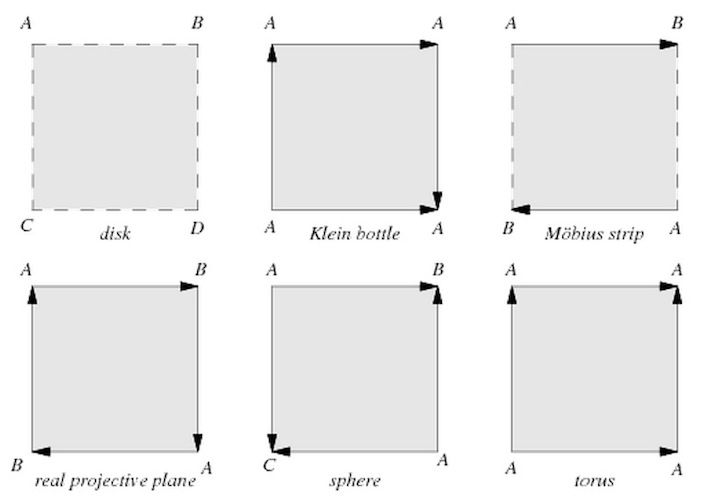
\includegraphics[width=0.6\textwidth]{topology_examples.jpg}
\caption{Connectivities of prominent 2D manifolds.}
\label{fig:topology_examples}
\end{figure}\\
Although topology is a comparatively young field in the history of mathematics, it would be futile trying to give a comprehensive explanation of the entire field\footnote{ The beginnings of Topology are closely related to advances in set theory at the end of the $19^{th}$ century. An iconic date for the commencement is the formal definition of metric spaces by \textit{Maurice Fréchet} in 1906. Today topology can be divided into algebraic topology (which includes combinatorial topology), differential topology, geometric topology and low-dimensional topology known as point-set topology \citep[][cf. p.2]{Weisstein2012}.}.\\
For our purposes we split this chapter in two parts, firstly we introduce the most important definitions in section \ref{math1}.
Many of the presented concepts will be already known, at least in an intuitive way, but in order to proceed to more demanding theories, it is necessary to formulate them in an concise and unifying manner.
Key ingredient is the notion of 'Simplicial Complexes' in \ref{math_simplicalcomplexes}, a powerful abstraction for spaces with triangulations, subsequently constructed by gluing together series of lower-dimensional simplices.\\
The second chapter \ref{math2} then will introduce a set of mathematical tools to describe and compute geometric features like handles and tunnels in a precise and rigid way.
As a means to do this, it will be necessary to introduce advanced theories like 'Filtration' and 'Topological Persistence', first described by Edelsbrunner \citep[cf.][]{Edelsbrunner2000}.
Some of the definitions might seem overly abstract at times, but as it turns out, describing and finding handles or tunnels in a mathematically sound manner is a challenging task.

What we ultimately want to achieve, by mobilizing all the mathematical machinery, is best expressed by the relation expressed in equation \ref{mother_equation}:
\begin{equation}
	\underbrace{ \chi = \sum (-1)^{n} \, \beta^{n}}_{Euler-Poincaré}
	\hspace{3ex} \longrightarrow \hspace{1ex}
	\underbrace{ \beta^{n}}_{n-Betti} =
	\underbrace{ rank ~{Z}^{n} - rank ~\mathrm{B}^{n}}_{Homology~groups} =
	\underbrace{ |\Prefix^{+}{\sigma^{n}}|-|\Prefix^{-}{\sigma^{n+1}}|}_{Filtration}
\end{equation}\\
In a nutshell what it says, is that the topological important information is connected to the filtration of simplices.
The Euler-Poincaré characteristic representing the topological important information can be calculate with Betti numbers.
This conclusion can be further used because the Betti numbers in turn, represent ranks of homology.
In other words, at the end we want to find groups of chains and circles that are either trivial or bounding.
All of that and more will be covered in this chapter.
%Figure
%\begin{figure}[ht]
%\centering
%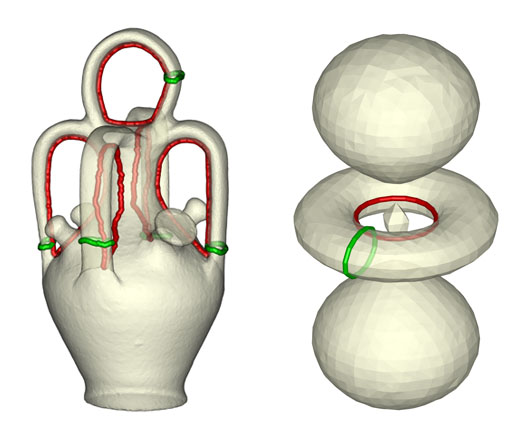
\includegraphics[width=0.1\textwidth]{loops_handles.jpg}
%\caption{Tunnel (red) and handle (green) loops \citep[cf.][]{Dey2012}.}
%\label{fig:loops_handles}
%\end{figure}\\

Note that the following expositions are somewhat informal in so far that they focus on conveying the concepts rather than building a strict series of deductions.
Lemmata or proofs will only be given if they are of importance for the understanding, further details and side-notes generally refer to sections in the appendix.

\newpage
\section{Mathematical Primer}
\label{math1}

Before we introduce any concepts it is important to stress that the field of topology is of axiomatic nature.
Therefore it can appear that already known structures are convoluted by cryptic terminology, but as often with axiomatic fields we have to accept these definitions as new.
For example, we mostly imply metric spaces when talking about ``a space'', when the differences are actually quite profound, see figure \ref{fig:spaces}:
%Figure
\begin{figure}[ht]
\centering
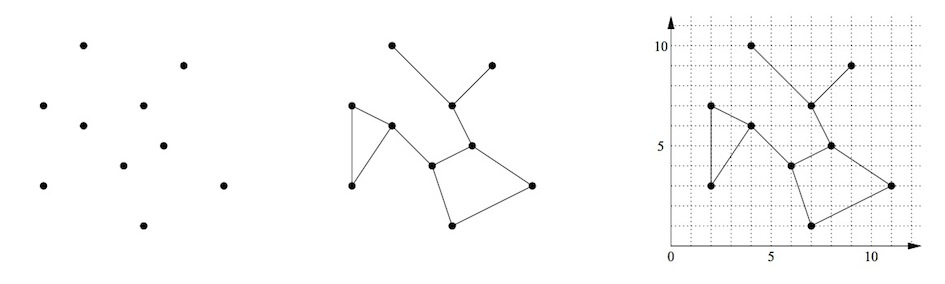
\includegraphics[width=0.95\textwidth]{spaces.jpg}
\caption{A point-, topological- and metric-space.}
\label{fig:spaces}
\end{figure}\\
A space can be a set of points without any structure.
For a topological space we need knowledge of the connectivity of the space, each point \textit{knows} which points are near it, that is its neighborhood.
To form a metric space we additionally need an associated metric, which enables us to measure distances and in turn, implicitly
defines neighborhoods.
Consequently any metric space is a topological one.
This means the geometry and topology of a space are fundamentally related, as they are both properties of a certain space.
However, the questions we are interested in are often topological in nature, and we may solve them easier by focusing on the topology and not on its geometry.
To do so, we need to identify intrinsic properties of spaces, especially the ones that are not changing -- so called invariants of the space\footnote{ This definition, to classifying geometries by their underlying symmetry groups, was coined by \textit{Felix Klein} (1849-1925) under the name ``Erlanger Programm''.
\begin{quote} \textit{``... Euclidean metric geometry can be described as the study of properties unchanged be the group of all rigid motions. ... All of these characteristics are dependent on two fundamental invariants in terms of which that can be expressed, namely, distance and angle. Euclid's pure geometry of measurement assumed that the effects of motion must leave size invariant. The issue of whether this is a good assumption for motion in the real world arises in twentieth-century physics.''} \citep[p.405]{Kramer1982} \end{quote}
} \citep[][cf. pp.1-5]{Zomorodian1996}.

\subsection{Topology}
\label{math_topology}

A topology is simply a system of sets that describe the connectivity of a set.
Formally a topology on a set $\mathrm{X}$ is a subset $\mathrm{T} \subseteq 2^{X}$ such that\footnote{ Definitions and figures in this chapter stem from mainly three resources and won't be cited individually:\begin{itemize}
\item \citep[][]{Hatcher2002} is a freely available textbook on algebraic topology and very often cited.
\item \citep[][]{Zomorodian1996} the PhD thesis of Prof. Afra Zomorodian, which features an extensive introductory chapter on topology (often citing Hatcher).
\item \citep[][]{Weisstein2002} the online resources of MathWorld, written and curated by \textit{Eric W. Weisstein}, hosted/sponsored by and licensed to 'Wolfram Research, Inc'.\end{itemize}}:
\begin{enumerate} \setlength{\itemsep}{0cm} \setlength{\parskip}{0cm}
	\Item $\text{If } \mathrm{A_{1}}, \mathrm{A_{2}} \in \mathrm{T} \text{, then } \mathrm{A_{1}} \cap \mathrm{A_{2}} \in \mathrm{T}.$
	\Item $\text{If } \{\mathrm{A_{j}} | j \in J\} \subseteq \mathrm{T} \text{, then } \cup_{J} \mathrm{A_{j}} \in \mathrm{T}.$
	\Item $\emptyset, \mathrm{X} \in \mathrm{T}.$
\end{enumerate}
We endow a set with structure to get the pair $\mathbb{X} = (\mathrm{X},\mathrm{T})$, called a topological space with any $\mathrm{A}_{i} \in \mathrm{T}$ an open set and its complements in $\mathrm{X}$ closed.
A continuous function between two topological spaces $f: \mathbb{X}_{1} \rightarrow \mathbb{X}_{2}$, is called a map if for every open set $\mathrm{B} \in \mathbb{X}_{2}$, $f^{-1}(\mathrm{B})$ is also open in $\mathbb{X}_{1}$, i.e. for every object in $\mathbb{X}_{2}$ exists an unique object in $\mathbb{X}_{1}$.\\
A homeomorphism $f: \mathbb{X}_{1} \rightarrow \mathbb{X}_{2}$ is a 1-1 onto function such that both $f$ and $f^{-1}$ are continuous, i.e. they have the same topological type $\mathbb{X}_{1} \approx \mathbb{X}_{2}$.
Homeomorphisms partition the class of topological spaces into equivalence classes and a fundamental problem in topology is characterizing these classes of homeomorphic spaces.

\subsection{Manifolds}
\label{math_manifolds}

A topological space may be viewed as an abstraction of a metric space.
Similarly, manifolds generalize the connectivity of $n$-dimensional Euclidean spaces $\mathbb{R}^{n}$ by being locally similar, but globally different, thus allowing to describe more complicated structures in terms of well-understood properties of Euclidean space.
A homeomorphism mapping the local ``area'' $\mathrm{U} \subseteq \mathbb{X}$ to an open subset of $\mathbb{R}^{n}$ is called a chart: $\varphi : \mathrm{U} \rightarrow \mathbb{R}^{n}$.
Formally a manifold is a topological space with a chart defined for every $x \in \mathbb{X}$.\\
For example, all neighborhoods on the 2-sphere $\mathcal{S}^{2}$ are homeomorphic to open disks.
Likewise the circle or 1-sphere $\mathcal{S}^{1}$ is a 1-manifold as every point has a neighborhood homeomorphic to an open interval in $\mathbb{R}^{1}$.
It is also the only compact 1-dimensional manifold.
Manifolds are generally the only topological spaces we are interested in.
%Figure
\begin{figure}[ht]
\centering
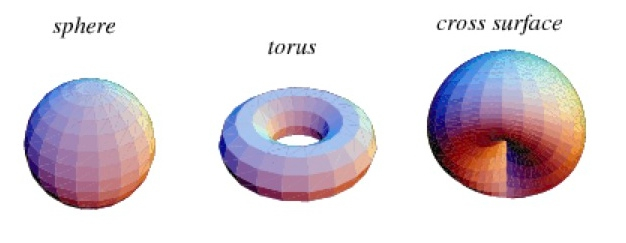
\includegraphics[width=0.60\textwidth]{manifolds.jpg}
\caption{Complete homeomorphism list for compact, boundaryless 2-dim. manifolds.}
\label{fig:manifolds}
\end{figure}\\
Another important attribute is compactness: A compact manifold can be embedded in $\mathbb{R}^{n}$ if it has finite extent, i.e. it can be covered by finitely many charts $\varphi_{n}$ -- thus all compact surfaces are triangulable \citep[which was first shown by][]{Rado1925}.
Compact manifolds in two dimensions are completely classified by two further attributes, namely orientation and genus, see picture \ref{fig:manifolds} and table \ref{tab:manifolds}:
\begin{table}[hbt]
\medskip
\setlength{\tabcolsep}{15pt}
\renewcommand{\arraystretch}{1.0}
   \centering
\begin{tabular}{ l || c | c | c } \centering
	\textbf{genus}		& 0			& 1				& 2 \\ \hline \hline
	\textbf{orientabel}	& sphere		& torus 			& double torus \\ \hline
	\textbf{nonorientable}	& -			& cross-cap		& Klein bottle \\
\end{tabular}
   \medskip
   \caption{Classes of 2-dimensional compact manifolds with low genus.}
   \label{tab:manifolds}
\end{table}\\
The genus is maybe the best known invariant property, as it intuitively describes the number of holes in a surface and we will see its connection to the more general notion of the Euler characteristic\footnote{ In higher-dimensional manifolds, the Euler characteristic is replaced by the concept of Betti numbers and homology/cohomology, as it gives rise to a broader framework of invariants, called functors. For definitions of homology and Betti numbers, see section \ref{math_homology}, respectively the glossary in appendix \ref{appendix_glossary}.} later in section \ref{math_euler}.
The genus can also be seen as the maximum number of cuttings along non-intersecting closed simple curves that can be drawn on the surface without disconnect the manifold into two.\\
The second invariant, orientability, describes whether it is possible to give all local charts $\varphi_{n}$ an ordering of either right- or left-handedness, without any two neighboring charts disagreeing globally.
Formally we will define this concept in the next section \ref{math_simplicalcomplexes}.\\
Using the connected sum, the homeomorphism problem is fully resolved for 2-manifolds\footnote{ \textit{Grigori Perelman} showed that 3-manifolds can also be decomposed into pieces with uniform geometry, whereas the problem is proven to be undecidable for higher dimensions \citep[][]{Morgan2007}.}, as every compact surface is homeomorphic to a sphere, the connected sum of tori, or the connected sum of cross surfaces\footnote{ Hence for any closed 2-manifold embedded in 3-dimensional space that can not be oriented, it follows, that it must have at least one self-intersection and any orientable 2-manifold without boundary is homeomorphic to a sphere with $n$-handles, i.e. its genus.}!

\subsection{Simplical Complexes}
\label{math_simplicalcomplexes}

At the beginning of the chapter in picture \ref{fig:topology_examples} we have seen that a torus, like a projective plane\footnote{ A sphere with one cross-cap has traditionally been called a real projective plane. The cross-cap is one of the three possible surfaces obtained by sewing a Möbius strip to the edge of a disk -- the other two are the Boy surface and Roman surface, see picture \ref{fig:nonorientable_surfaces}. A sphere with two cross-caps having coinciding boundaries is topologically equivalent to a Klein bottle.} and a sphere, all can be obtained from a
square by identifying the edges with certain directions and gluing them together accordingly.
Cutting a square trivially along a diagonal produces two triangles that can be easily further subdivided, so each of these surfaces in turn can be reduced to triangles.
Together with the result from the last section \ref{math_manifolds}, that all compact 2-manifolds can be assembled by combining spheres, tori and cross-caps, we have proven that in fact all closed surfaces can be constructed from triangles.\\
Thus we have a single building block to construct a large class of 2-dimensional spaces and the idea now is to generalize this for any dimension:
The $n$-dimensional analog of the triangle is the convex hull of $n$+1 affinely independent points $\mathcal{V} = \{v_{0}, v_{1}, \dots , v_{n}\}$, it is called the $n$-simplex: $\sigma^{n}_{i}$, with $n$ and $i$ denoting the dimension and index: $i,n \in \mathbb{N}$.
Simplices have familiar names for low dimensions, see figure \ref{fig:n-simplices}:
%Figure
\begin{figure}[ht]
\centering
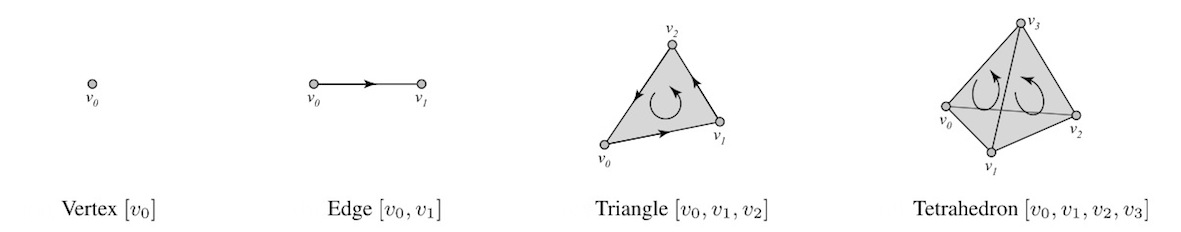
\includegraphics[width=1.0\textwidth]{n-simplices.jpg}
\caption{Oriented $n$-simplices, $0 \leq n \leq 3$.}
\label{fig:n-simplices}
\end{figure}\\
Now a simplicial complex $\mathrm{K}$, is a finite set of simplices such that every subset $\mathrm{T} \subseteq \mathcal{V}$ is also in $\mathrm{K}$, and the nonempty intersection of any two simplices, again is a subset in $\mathrm{K}$.
The dimension $n$ of $\mathrm{K}^{n}$ is defined as the maximum dimension of its simplices: $max_{n}\{\sigma^{n}_{i}\}$.\\
That is to say, that a simplicial Complex is a set of elements, i.e. simplices of different dimension, that built up and represent a manifold.
The cumbersome definition stems from the fact that we want to exclude certain ill-formed sets, shown in figure \ref{fig:simplical_complexes}.\\
To put this into context, a triangulation of a topological space $\mathbb{X}$ is a simplicial complex $\mathrm{K}$.
Formally this is the case if the underlying space of the simplicial complex is isomorphic to the topological space: $||\mathrm{K}|| \approx \mathbb{X}$.
Thus, two simplicial complexes $\mathrm{K}$ and $\mathrm{L}$ are isomorphic if and only if their topological spaces are: $\mathbb{X}_{\mathrm{K}} \approx \mathbb{X}_{\mathrm{L}}$.
%Figure
\begin{figure}[ht]
\centering
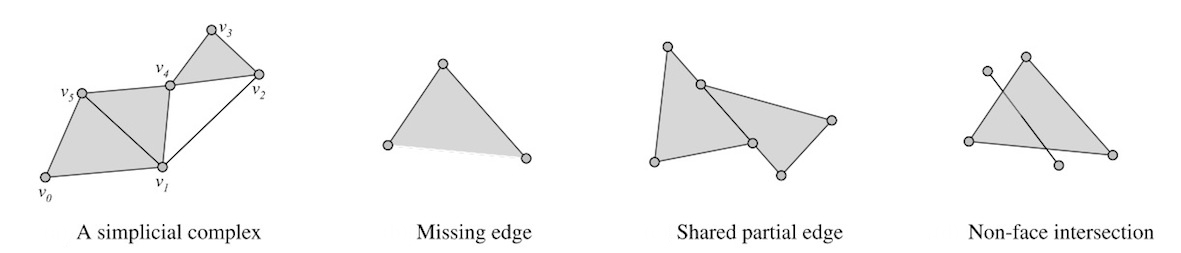
\includegraphics[width=1.00\textwidth]{simplical_complexes.jpg}
\caption{One simplicial complex and three unions that are not complexes.}
\label{fig:simplical_complexes}
\end{figure}\\
For purposes of homology it is important to keep track of the order of the simplices, so $n$-simplex really means $n$-simplex with ordering, which as a by-product, determines orientation:
Two $n$-simplices sharing a ($n$-1)-simplex are consistently oriented if they induce different orientations.
A triangulable $n$-manifold is orientable if all simplices can be oriented consistently, otherwise it is nonorientable, see figure \ref{fig:nonorientable_surfaces}.
Orientations are normally graphically indicated by using arrows, as shown in figure \ref{fig:example_orientation}.
Note that in three dimensions, there is no unbounded non-orientable surface which does not intersect itself\,\footnote{ See appendix \ref{appendix7}, for a very elegant proof of this statement.}.
%Figure 
\begin{floatingfigure}[r]{0.30\textwidth}
\centering
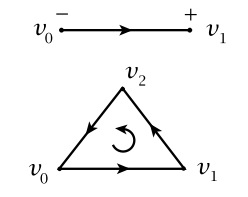
\includegraphics[width=0.25\textwidth]{example_orientation.jpg}
\caption{Orientation.}
\label{fig:example_orientation}
\end{floatingfigure}
We can generalize the idea now for any dimension $n \geq 1$:
Then an orientation of a $n$-simplex $\sigma^{n}$, is an equivalence class of orderings, written $[\sigma]$, of its vertices: $\sigma = \{v_{0}, v_{1}, \dots , v_{n}\}$, where: $(v_{0}, v_{1}, \dots , v_{n}) \sim (v_{\tau(0)}, v_{\tau(1)}, \dots , v_{\tau(n)})$, are equivalent orderings if the parity of the permutation $\tau$ is even\footnote{ For any finite set $\mathrm{X}$ with an ordering and at least two elements, the bijective mapping $\tau : \mathrm{X} \rightarrow \mathrm{X}$, falls into two classes of equal size, i.e. the even and odd permutations. The parity a permutation is then defined as the number of inversions for $\mathrm{N}(\tau)$, of pairs of elements $x_{i}, x_{j} \in X$, such that $x_{i} < x_{j}$ but $\tau(x_{i}) > \tau(x_{j})$, intuitively this denotes the number of occurred swaps.}.\\
It is worth noting that simplicial complexes, by definition, are combinatorial objects with topology and don't necessarily have to utilize geometry.
If the topology gets separated, $\mathrm{K}^{*}$ is called an abstract simplicial complex\footnote{ Actually written down for simplicial complexes, the mathematical definition of this vertex scheme, strikingly resembles the connectivity list of an \textit{.obj}, \textit{.ply} or \textit{.off} file.}.
%Figure
\begin{figure}[ht]
\centering
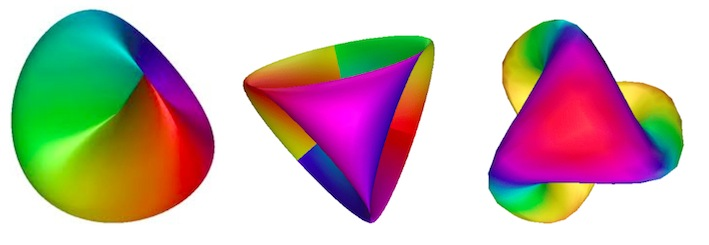
\includegraphics[width=0.45\textwidth]{nonorientable_surfaces.jpg}
\caption[Non-orientable surfaces]{Basic non-orientable surfaces: Cross-cap, Roman and Boy surface.}
\label{fig:nonorientable_surfaces}
\end{figure}

\subsection{General Euler Characteristic}
\label{math_euler}

Next to orientability the genus is the second most well known invariant for classifying $2-$manifolds.
We already have a intuitive notion for it, as it represents the number of holes\footnote{ Though even for non pathological cases it can be very hard to ``see'' the genus of a given surface. A famous example is the so called ``House with two rooms'', illustrated in appendix \ref{two_rooms}.}, but with simplicial complies at our disposal we can formulate this concept in a generalized and formal adequate way for any $n$-manifold.\\
The Euler characteristic is defined for a simplicial complex $\mathrm{K}$ with $|\sigma^{n}|$ finitely many $n$-simplex as the number of even- minus the number of odd-dimensional simplices:
\begin{equation} \label{eq:euler_characteristic}
\chi(\mathrm{K}) = \sum_{n = 0}^{dim \mathrm{K}} (-1)^{n} |\sigma^{n}|
\end{equation}
Which in the $2$-dimensional case leads to the well known relation:
\begin{equation*}
\chi(\mathbb{M}_{2}) = |\sigma^{0}| - |\sigma^{1}| + |\sigma^{2}| = vertices - edges + faces
\end{equation*}
And we get for the tetrahedron $\sigma^{3}$ in picture \ref{fig:simplical_complexes}: $\chi(\sigma^{3}) = 4 - 6 + 4 = 2$, which by definition is a triangulation of the sphere $\mathcal{S}^{2}$, thus defining the homeomorphism for any convex polyhedron $\mathbb{M}$ as $\chi(\mathbb{M}) = 2$, respectively $\chi(\mathbb{M}) \simeq \chi(\mathcal{S}^{2})$.\\
The Euler characteristic of a $\mathrm{K}$ depends only on its homotopy type, no matter how it is geometrically represented, i.e.
it is an integer invariant for $|\mathrm{K}|$, the underlying space.
We already know that any compact orientable surface is homeomorphic to a sphere or $n$ connected tori.
Thereby we can give an atomic formula for any connected sums of orientable $\mathbb{M}_{sum}$ or nonorientable $\mathbb{N}_{sum}$ manifolds\footnote{ An informal explanation for the added $(-2g)$ and $(-g)$ terms is, that, to connect the surfaces one either has to cut out a disk on either tori $(-2)$, or cut two disks and insert a projective plane $(-2+1)$, g-times.}: 
\begin{equation}
\chi(\mathbb{M}_{sum}) = 2 - 2g \text{, respectively: } \chi(\mathbb{N}_{sum}) = 2 - g
\end{equation}
%Figure
\vspace*{-4ex}
\begin{figure}[ht]
\centering
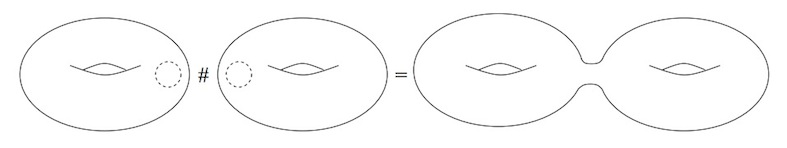
\includegraphics[width=0.8\textwidth]{connected_sum.jpg}
\caption{A double torus, as the connected sum of two tori.}
\label{fig:connected_sum}
\end{figure}

\subsection{Homotopy}
\label{math_homotopy}

Two continuous functions from one topological space to another are called homotopic, if one can be continuously deformed into the other.
The deformation then is called the homotopy between the two functions and an equivalence relation on topological spaces\footnote{ Equivalence classes under $\simeq$ are called homotopy types. Like any equivalence relation they partition a set so that every element of the set is a member of one and only one cell of the partition. The intersection of any two different cells must be empty and the union of all the cells equals the original set. They are reflexive: $\mathrm{X} \simeq \mathrm{X}$, symmetric: $\mathrm{X} \simeq \mathrm{Y} \, \Rightarrow \, \mathrm{Y} \simeq \mathrm{X}$ and transitive: $\mathrm{X} \simeq \mathrm{Y} \, \& \, \mathrm{Y} \simeq \mathrm{Z} \Rightarrow \mathrm{X} \simeq \mathrm{Z}$.}.
More precisely, two continuous maps $f, g: \mathbb{X}_{1} \rightarrow \mathbb{X}_{2}$ are homotopic, if a continuous function exists $\mathrm{F}: \mathbb{X}_{1} \times [0,1] \rightarrow \mathbb{X}_{2}$, so that:
\begin{equation}
	\mathrm{F}(x, 0) = f(x) \text{ and } \mathrm{F}(x, 1) = g(x) \text{, for all } x \in \mathbb{X}_{1}
\end{equation}
To give an example: Any two continuous real functions $f, g: \mathbb{R} \rightarrow \mathbb{R}$ are trivially homotopic via $\mathrm{F}(x,t) = (1-t) \cdot f(x) + t \cdot g(g)$.
If $f$ is homotopic to a constant map, i.e. $f \simeq const.$, then $f$ is called nullhomotopic.
As with functions, two spaces $\mathbb{X}_{1}$ and $\mathbb{X}_{2}$ are homotopy equivalent if they can be transformed into one and another by continuous bending, shrinking and expanding operations, see picture \ref{fig:homotopy}.
%Figure
\begin{figure}[htb]
\centering
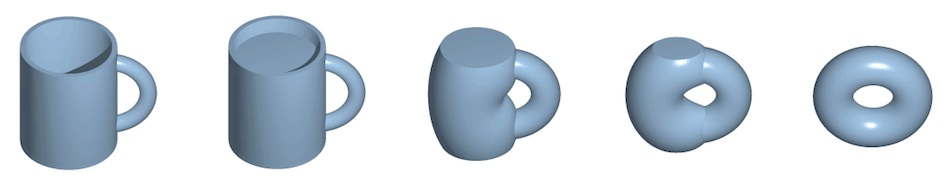
\includegraphics[width=0.9\textwidth]{homotopy.jpg}
\caption{A famous example for homotopic equivalence are a coffee cup and a torus.}
\label{fig:homotopy}
\end{figure}\\
A topological space $\mathbb{X}$ is said to be contractible or nullhomotopic if $\mathbb{X}$ is homotopy equivalent to a point, i.e. $\mathbb{X} \simeq \sigma^{0}$.\\
It is important not to mix up homeomorphism with homotopy.
For example, a cylinder is not homeomorphic to a circle, but homotopy equivalent to it, as it may continuously be shrunken via a deformation retraction\footnote{ Deformation retraction is a special case of a homotopy, with the requirement that the target space is a subspace. The retraction of a space $\mathbb{X}$ onto a subspace $\mathrm{A}$ is a family of continuous maps $f_{t}: \mathbb{X} \rightarrow \mathrm{A}, t \in [0,1]$, so that $f_{0}$ is the identity map: $f_{0}(\mathbb{X}) = \mathbb{X}$, and $f_{1}(\mathbb{X}) = \mathrm{A}$. In other words, starting from the original space $\mathbb{X}$ at time $0$, we continuously deform the space until it becomes the subspace $\mathrm{A}$ at time $1$. This is done without ever moving the subspace $\mathrm{A}$ in the process.}.
Thus, two spaces with a different topological type can still have the same homotopy type, but all homeomorphic spaces are homotopic: $\mathbb{X}_{1} \approx \mathbb{X}_{2} \, \Rightarrow \, \mathbb{X}_{1} \simeq \mathbb{X}_{2}$ but not the other way around.

\subsection{The Fundamental Group}
\label{math_fundamental_group}

We saw in the last section that two maps are homotopic if one can be continuously deformed into the other.
Now this idea gets applied to maps on surfaces, called paths.
Paths that begin and start at the same basepoint $x_{bp}$, namely loops, are of special concern and used to characterize the so called fundamental group.\\
Loops that are boundaries of a disk are contractible and belong to the same class as the trivial loop, which never leaves its basepoint.
If we find non-bounding loops, they form a different class, see picture \ref{fig:fundamental_group_torus}.
%Figure
\begin{figure}[htb]
\centering
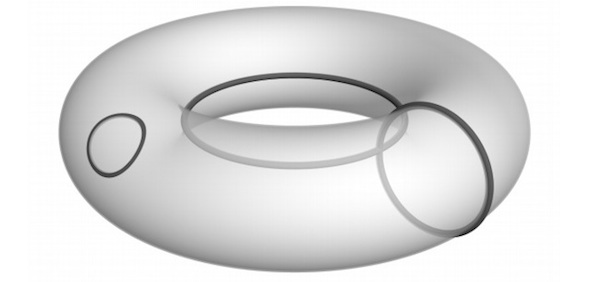
\includegraphics[width=0.45\textwidth]{fundamental_group.jpg}
\caption{One boundary loop (on the left) and two non-bounding loops on a torus.}
\label{fig:fundamental_group_torus}
\end{figure}
\begin{equation}
	f_{loop}: [0,1] \rightarrow \mathbb{X} ~~ \text{ with }~~ f_{loop}(0) = x_{bp} = f_{loop}(1)
\end{equation}
The non-bounding loops define the fundamental group.
Formally the fundamental group of a topological space is the group formed by the set of equivalence classes of all loops with the same initial and final basepoint, under the equivalence relation of homotopy:
\begin{equation}
	\pi(\mathbb{X}, x_{bp}) = \{ f_{loop}: [0,1] \rightarrow \mathbb{X} ~|~ f_{loop}(0) = x_{bp} = f_{loop}(1)\}_{h}
\end{equation}
For a non-pathological spaces, i.e. path-connected spaces, the basepoint is irrelevant and we refer to the group as $\pi_{1}(\mathbb{X})$.
For example, any loop drawn on the sphere is bounding, so $\pi_{1}(\mathcal{S}^{2}) \cong \{0\}$ where $\cong$ denotes group isomorphism\footnote{ Admittedly, it is hard not to get confused by all the introduced -morphisms (left alone, that there are even more esoteric ones). Isomorphism is a bijective group homomorphism, which in turn must not be confused with homeomorphism. Contrary to homeomorphism, homomorphism is structure-preserving.} and $\{0\}$ is the trivial group.\\
Each homotopy class consists of all loops which wind around the circle a given number of times.
So the fundamental group of the circle is isomorphic to the additive group of integers $\mathbb{Z}$.
Intuitively then, $\pi_{1}(\mathcal{S}^{1}) = \mathbb{Z}$ and similarly the two non-bounding loops in picture \label{fig:fundamental_group} generate the fundamental group of a torus: $\pi_{1}(\text{Torus}) \cong \mathbb{Z} \times \mathbb{Z}$.\\
The fundamental group, in fact, measures the 1-dimensional hole structure of a space.
Following is table \ref{tab:fundamental_group} of the fundamental group for some common spaces:
\begin{table}[htpb]
\medskip
\setlength{\tabcolsep}{25pt}
\renewcommand{\arraystretch}{1.25}
   \centering
\begin{tabular}{ l | c | c } \centering
	\textbf{Space}	& \textbf{Symbol}				& \textbf{$\pi_{1}$} \\ \hline \hline
	Circle			& $\mathcal{S}^{1}$			& $\mathbb{Z}$ \\
	Torus			& $\mathcal{T}^{2}$			& $\mathbb{Z}^{2}$ \\
	Projective plane	& $\mathbb{R}\mathrm{P}^{2}$	& $\mathbb{Z}$ \\
	Sphere			& $\mathcal{S}^{2}$			& $0$ \\
\end{tabular}
	\bigskip
	\caption{Fundamental group for various spaces.}
	\label{tab:fundamental_group}
\end{table}\\
The fundamental group is one in a series of homotopy groups $\pi_{n}(\mathbb{X})$ that study higher dimensional holes.
The homotopy groups $n > 1$ extend the notion of a loop to $n$-dimensional circles and capture the homotopy
classes of these circles.

\subsection{Chains and Circles}
\label{math_chainloops}

As before, we can now generalize the concept of paths and loops with the help of simplicial complexes and use it to define another topological invariant, homology.\\
A path $c$ constructed with simplices of dimension $n$ is called a $n$-chain of the simplicial complex $\mathrm{K}$.
With $\sigma_{i}^{n} \in \mathrm{K}, ~k_{i} \in \mathbb{Z}$ and the brackets $[\cdot]$ indicating orientation as introduced in section \ref{math_simplicalcomplexes}, we define a $n$-chain as the sum of $i$ connected simplices:
\begin{equation}
	\mathrm{c}^{n} = \sum_{i} k_{i} [\sigma_{i}^{n}] ~\text{ respectively the chain group of all $n$-chains: } \mathrm{C}^{n} = \{ \cup_{\mathrm{K}} ~ \mathrm{c}^{n} \}
\end{equation}
We also define a commutative addition for chains with integer coefficients modulo 2.
In other words, the sum of two $n$-chains $c$ and $d$ is the symmetric difference of the two sets: $c+d = (c \cup d) - (c \cap d)$, preventing multiple instances of an element $\sigma^{n}$ in the set.\\
The chain group $\mathrm{C}^{n}$ is the set\footnote{ To be precise, this set forms a free Abelian group on the oriented $n$-simplices: $\langle \mathrm{C}^{n}, + \rangle$. Which means, they form a basis and the entirety of the elements can be written as linear combinations of the basis.\\ Abelian groups are structures of abstract algebra, studied in group theory. As we are interested in characterizing the topology of spaces, group theory is a related classification systems that yields many interconnections. Although promising powerful tools to define equivalence relations, the exploration of this relation is beyond the scope of this thesis and my knowledge thereof \citep[for an in depth introduction to the field of geometric group theory, see][]{Stillwell1993}.} of all chains with dimension $n$, hence $\mathrm{K}$ has a chain group in every dimension.
These chain groups $\mathrm{C}^{n}$ are structurally related in the way that $(n\text{-1})$-chains form the boundaries of $n$-chains, i.e. every tetrahedron $\sigma^{3}$ is bounded by four triangles $\sigma^{2}_{\{1-4\}}$ and every triangle $\sigma^{2}$ is bounded by three edges $\sigma_{\{1-3\}}^{1}$ and so forth.
We now define this relation formally via the boundary operator:
\begin{equation} \label{eq:boundary}
	\partial \,\sigma^{n} = \partial \,\{ v_{0}, \dots , v_{n} \} = \sum_{i}^{n} \,\{v_{0}, \dots, \hat{v}_{i}, \dots, v_{n}\}
\end{equation}
where $\hat{v}_{i}$ is the simplex that gets deleted from the sequence.
We extend this operator to entire chain groups, $\partial_{n}: \mathrm{C}^{n} \rightarrow \mathrm{C}^{n-1}$ and interpret $\partial_{0} \equiv \emptyset$.
The entire series of the groups that are connected via the boundary operator is then called a chain complex $\mathrm{C}^{\mathrm{K}}$ : $\mathrm{C}^{\mathrm{K}} = \mathrm{C}^{n} \overset{\partial_{n}}{\longrightarrow} \mathrm{C}^{n-1} \overset{\partial_{n-1}}{\longrightarrow} \dots \overset{\partial_{1}}{\longrightarrow} \mathrm{C}^{0} \overset{\partial_{0}}{\longrightarrow} \emptyset$\\
This gives us the definition of a $n$-circles as $n$-chains that have no boundary.
As an example consider the triangle in figure \ref{fig:example_orientation}, with the obvious $1$-circle, formed by its edges: $\partial_{2} \sigma^{2} = \partial_{2} \{ \sigma^{1}_{0}, \sigma^{1}_{1}, \sigma^{1}_{2} \} = \{v_{1}, v_{2}\} + \{v_{0}, v_{2}\} + \{v_{0}, v_{1}\}$, now taking the boundary of the boundary we can see: $\partial_{1} (\{v_{1}, v_{2}\} + \{v_{0}, v_{2}\} + \{v_{0}, v_{1}\}) = 2v_{2}+2v_{1}+2v_{0}$ and with the addition defined modulo 2, the results is: $2v_{2}+2v_{1}+2v_{0} = \emptyset$.
This is intuitively correct, as the boundary of a triangle is a cycle, and a cycle does not have a boundary.
In fact, this intuition generalizes to chain groups of any dimension\footnote{ We omit the proof, but it is rather straight forward, as $\partial_{n} \partial_{n-1} = \sum \sum [\dots]$ mod2 always cancels out.}: $\partial_{n}(\partial_{n-1}) = \emptyset$.
In other words, the $n$-cycles are the kernel\footnote{ The boundary operator $\partial_{n}$ is a group homomorphism, hence the kernel is defined as the set of all elements which are mapped to the identity element of $\partial_{n-1}$. The image, analogous to real functions, is the range of all mapped elements, i.e. all chains for which $\partial_{n+1}$ is defined.} of $\partial_{n}$ and thereby form a subgroup of the chain group $\mathrm{C}^{n}$, which is called the cycle group: $\mathrm{Z}_{n} = ker ~ \partial_{n} = \{ c \in \mathrm{C}^{n} ~ | ~ \partial_{n} \, c = 0\}$.\\
If we recall the three circles on the torus shown in figure \ref{fig:fundamental_group_torus}, we see that apart from the boundary loops, there are also non-bounding loops.
The entirety of loops can be defined by the image of all ($n$+1)-boundaries: $\mathrm{B}_{n} = im ~ \partial_{n+1} = \{ c \in \mathrm{C}^{n} ~|~ \exists d \in \mathrm{C}^{n+1} : c = \partial_{n+1}(d) \}$.
%Figure
\begin{figure}[htb]
\centering
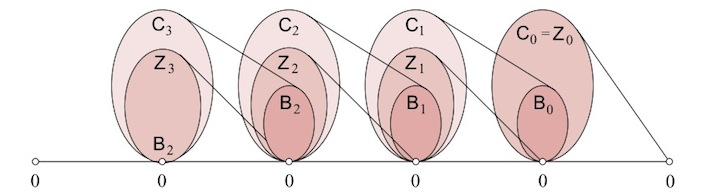
\includegraphics[width=0.70\textwidth]{chain_complex.jpg}
\caption{The chain complex for a $3$-dimensional simplicial complex.}
\label{fig:chain_complex}
\end{figure}\\
In other words, for any dimension $n$ of $\mathrm{K}$, there exist chains of simplices: $\mathrm{C}^{n}$, of which some form loops: $\mathrm{Z}^{n}$ and of those some are bounding: $\mathrm{B}^{n}$, hence: $\mathrm{C}^{n} \supseteq \mathrm{Z}^{n} \supseteq \mathrm{B}^{n}$, see \ref{fig:chain_complex}.

\subsection{Homology Groups \& Betti Numbers}
\label{math_homology}

We have $n$-chains and $n$-cycles, which are simplicial analogs of paths and loops for $n\text{=1}$ in the continuous domain of topological spaces.
Following the construction of the fundamental group, we now need the simplicial version of homotopy to form equivalent classes of cycles on triangulated spaces, that is the homology group\footnote{  With $/$ the quotient set, which for $\mathrm{H}^{1}$ is the class of circles that are non-bounding, analogous to $\pi_{1}$.}: $\mathrm{H}^{n} = \mathrm{Z}^{n} / \,\mathrm{B}^{n} = ker ~\partial_{n} / \,im ~\partial_{n+1}$\\
The homology groups are invariants for $|\mathrm{K}|$ and for homotopy equivalent spaces.
This means formally, $\mathbb{X}_{1} \simeq \mathbb{X}_{2} \Rightarrow \mathrm{H}^{n}(\mathbb{X}_{1}) \cong \mathrm{H}^{n}(\mathbb{X}_{2})$ for all $n$.
However, for the rest of the thesis, we will only consider the first homology group $\mathrm{H}^{1}$, as it represent the circles we are interested in, especially the ones which constitute handle and tunnel loops.\\
One might ask, why we defined simplicial complexes and for that matter homology groups when they just resembles topological spaces and homotopy.
The crucial difference is, that homology is defined for non-continuous spaces, built out of simplices and therefore lends itself to feasible methods for computation.
In fact, if we extend homology groups with the definition of $rank(\mathrm{H}^{n})$, as the number of independent subsets, we get a full series of invariants, called the $n^{th}$ Betti number, with intuitive meanings for low dimensions:
\begin{equation} \label{eq:homology_betti}
	\beta^{n} = rank ~\mathrm{H}^{n} = rank ~{Z}^{n} - rank ~\mathrm{B}^{n}
\end{equation}
\vspace*{-6ex}
\begin{enumerate}
\setlength{\itemsep}{0pt}
\setlength{\parskip}{0pt}
\item[$\beta^{0}$] counts the number of connected components of the space.
\item[$\beta^{1}$] is the dimension of any basis for the loops.
\item[$\beta^{2}$] counts the number of enclosed spaces or voids.
\end{enumerate}
For example, the torus is one connected component, has two loops and encloses one void: $\beta^{0} = 1, ~\beta^{1} = 2, ~\beta^{2} = 1$, and $\beta^{n} = 0$ for all $n > 2$.
Note that the Betti numbers for the projective plane are defined, although it is not embeddable in $\mathbb{R}^{3}$ without intersecting itself\footnote{ \textit{Hiroshi Maehara} conceived an elegant proof, showing the impossibility of: $\mathrm{P}^{2} \hookrightarrow \mathbb{R}^{3}$, see appendix \ref{appendix7}.}, see table \ref{tab:betti_numbers}:
\begin{table}[hbt]
\medskip
\setlength{\tabcolsep}{15pt}
\renewcommand{\arraystretch}{1.15}
   \centering
\begin{tabular}{ l | c c c} \centering
	\textbf{Surface}	& $\mathrm{H}^{0}$	& $\mathrm{H}^{1}$	& $\mathrm{H}^{2}$ \\ \hline
	Torus			& $\mathbb{Z}$		& $\mathbb{Z}^{2}$	& $\mathbb{Z}$ \\
	Sphere			& $\mathbb{Z}$		& $\{0\}$				& $\mathbb{Z}$ \\
	Projective plane	& $\mathbb{Z}$		& $\{0\}$				& $\{0\}$
\end{tabular}
	\medskip
	\caption{Homology groups for the basic surfaces.}
	\label{tab:betti_numbers} 
\end{table}

\subsection{The Euler-Poincaré Formula}
\label{math_euler_{poincare}}

The relevance of Betti numbers goes further then just applying the concept of homotopy to simplices.
To end this section, we derive the invariance of the Euler characteristic of section \ref{math_euler} from the invariance of homology\footnote{ Historically this idea gave rise to a famous conjecture, namely the so called Hauptvermutung. The hope was, that if two different simplicial complexes $\mathrm{K}$ and $\mathrm{L}$ are bound by a homeomorphism, i.e. $|\mathrm{K}| \approx |\mathrm{L}|$, it would translate to the homology of the spaces itself. In other words, if true, any two triangulations of a topological space have at least one common refinement, a single triangulation that is a subdivision of both of them. The general version of the conjecture was proven to be false, but the manifold version holds true for dimensions $dim \leq 3$ \citep[for an extensive discussion, see:][]{Ranicki1996}.}.
By doing this we introduce a bit more algebra and complexity than we might otherwise would have needed, but it will yield a reference of justification for the next chapter.\\
Recall that a simplicial complex $\mathrm{K}$, as a constructed object, breaks down into a chain complex $\mathrm{C}^{\mathrm{K}}$ of finite length.
The Euler characteristic $\chi(\mathrm{K})$, as defined in equation \eqref{eq:euler_characteristic}, is the alternating sum of the number of used simplices $|\sigma^{n}|$.
However, this is also the rank of the corresponding $\mathrm{C}^{n}$, as it is the group on oriented $n$-simplices that get generated by these very simplices.
Thus we can define the Euler characteristic in terms of the chain complex:
\begin{equation}
	\chi(\mathrm{K}) = \chi(\mathrm{C}^{\mathrm{K}}) = \sum_{n}^{dim\, \mathrm{K}} (-1)^{n}~ rank \,(\mathrm{C}^{n})
\end{equation}  
Maybe surprisingly, it can be shown\footnote{ For the proof, see \citep[][pp.155-156]{Hatcher2002}.} that $\chi(C^{\mathrm{K}}) = \chi(\mathrm{\mathrm{H}}(\mathrm{C}^{\mathrm{K}}))$, which means that the homology functor preserves the Euler characteristic of a chain complex.
With the equation \eqref{eq:homology_betti}: $rank ~\mathrm{H}^{n} = \beta^{n}$, we get the Euler-Poincaré formula:
\begin{equation} \label{eq:euler_poincare}
	\chi(\mathrm{K}) = \sum_{n}^{dim \, \mathrm{K}} (-1)^{n} \,|\sigma^{n}| =
	\sum_{n}^{dim\, \mathrm{K}} (-1)^{n}~ rank ~\mathrm{H}\,(\mathrm{C}^{n}) =
	\sum_{n}^{dim \, \mathrm{K}} (-1)^{n}\, \beta^{n}
\end{equation}
This relation, besides its intrinsic mathematical appeal, has important implications for us.
It means that we can derive the Euler characteristic by computing the Betti numbers. 
More importantly it shows that Betti numbers are intimately related to the topological concept of certain paths, namely circles.
And since tunnels and handles are described by circles, we have a connection between the former and the latter.
Hence, in order to find special geometric structures, we can study specific groups of circles that are by themselves distinguishable via the decomposition of their simplices!

\newpage
%\vspace*{1ex}
\section{Handles and Tunnels}
\label{math2}

The last section ended with the insight that circles, or rather loops as their 2-dimensional manifestations, are valid constructs to describe topological features.
However, this is not enough, not only would it be much easier to compute topological properties via the simple Euler characteristic, but moreover the description of topological features in itself is ``blind''.
What we are really interested in, after all, is the identification of specific geometric details.
Geometric details that come with certain topological traits, but in order to exploit circles for feature detection we need to employ the theory of topological persistence, which is a substructure of the more general Morse theory\footnote{ Morse Theory provides an analysis of the relationship between the geometry and the topology of a space. Though it was developed for smooth domains, it can be translated to simplicial complexes. It is a generalization of calculus of variations which seeks to find the path, curve, surface, etc. for which a given function has a stationary value. It draws on the relationship between the stationary points of a smooth real-valued function on a manifold and the global topology of the manifold. For example, if a compact manifold admits a function whose only stationary points are a maximum and a minimum, then the manifold is a sphere \citep[for an introduction, see:][]{Kitagawa2006}. Morse theory is related to the topology of Lie groups and has received much attention in the last decades, as it is important for the description of quantum field theory \citep[cf.][]{Witten1982}.}.
The theory identifies critical points at which level-sets of a function undergo topological changes, and relates these points via a complex -- note that: $\chi = 2 - 2g =$ \textit{minima - saddles + maxima}, see figure \ref{fig:morse_theory}:
%Figure
\begin{figure}[htb]
\centering
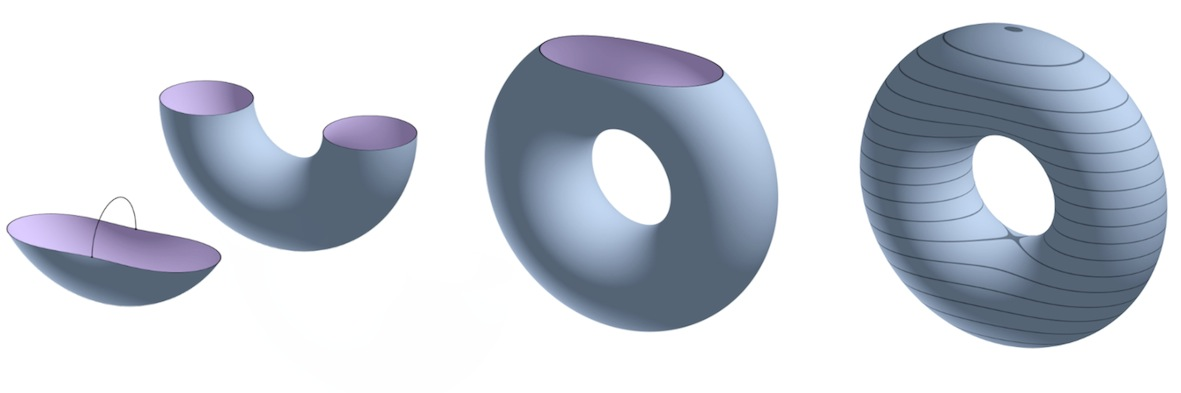
\includegraphics[width=0.90\textwidth]{morse_theory.jpg}
\caption{Morse theory -- starting from the bottom the homotopy type of the torus changes at its critical points from: point or disk, to cylinder, continues to a torus with a removed disk boundary, until it is finally a full torus.}
\label{fig:morse_theory}
\end{figure}\\
The rest of this chapter is split into the following sections: First we will survey previous work in \ref{math_loop_previous_work}, then in section \ref{math_loop_definition} we will proof that there is in fact, always a distinct class of circles that describe the geometric features we are interested in.
Afterwards we define topological persistence in section \ref{math_topological_persistance} and see how it may help us, and finally in \ref{math_loop_computation} we explain how to find the loops computationally.

\subsection{Previous Work}
\label{math_loop_previous_work}

Numerous papers have been published dealing with non-trivial loops on surfaces, as they hold important topological information.
For a good overview, see the references in \citep[][especially section 2]{Ni2004}.
For our thesis, we will focus on preceding work with a explicit context in simplification.
Below are some references with descriptions:
%List \vspace{-2ex}
\begin{itemize}
%\setlength{\itemsep}{0cm}
%\setlength{\parskip}{0cm}
	\item \citep[][]{El-Sana1997} \textit{``Controlled Simplification of Genus \dots''}\\
They identify holes and the concavities by extending the concept of $\alpha$-hulls\footnote{ Generalization for the concept of convex hulls as a set of points associated with disks that represent simple curves \citep[introduced by][]{Edelsbrunner1983}.} to polygonal meshes under the $\mathrm{L}_{\infty}$ distance metric and then triangulate parts of the surface that are not accessible for a ball of a defined radius.
	\item \citep[][]{Guskov2001} \textit{``Topological Noise Removal''}\\
Propose a surface growing strategy to find features and remove unnecessary non-trivial topology. They use a local wave front traversal to discover and identify small tunnels. Then they find and select non-separating cuts to sever and seal the mesh, thus reducing the genus.
	\item \citep[][]{Nooruddin2003} \textit{``Simplification \dots Using Volumetric Techniques''}\\
Describe a method for converting polygonal models to a volumetric representation. The topology altering part is based on 3D morphological operators that work in the volume domain.
	\item \citep[][]{Wood2004} \textit{``Removing Excess Topology From Isosurfaces''}\\
They find handles by incrementally constructing and analyzing Reeb graphs\footnote{ Named after \textit{Georges Reeb}, these graphs of a function describe the connectivity of its level sets -- for figure \ref{fig:morse_theory} the graph would be formed by two edges connected bottom and top of a circle.}. Handles are removed robustly by modifying the volume in a disk-filling procedure.
	\item \citep[][]{Dey2007} \textit{``On Computing Handle and Tunnel Loops''}\\
Using the concept of topological persistence, they filter a manifold to get a set of simplices that are linked to edges that form handle and tunnel loops.
The main advantage of this approach is, that unlike others, it can provide a mathematical guarantee to find relevant topological features without introducing artifacts.\\
Hence we follow this idea\footnote{ The work of \textit{Tamal K. Dey} was first brought to our attention in a discussion with \textit{Tamy Boubekeur}.} and built upon their work as described in section \ref{math_loop_computation}.
\end{itemize}

\subsection{Definition \& Existence of Handle and Tunnel Loops}
\label{math_loop_definition}

One goal for this thesis is, not only to preserve, but to control topology.
This entails mathematically having to define even very intuitive concepts like handles and tunnels.
Formally this was first done in reference to mesh simplification by \citep[][]{Dey2007}.
%Figure
\begin{figure}[htb]
\centering
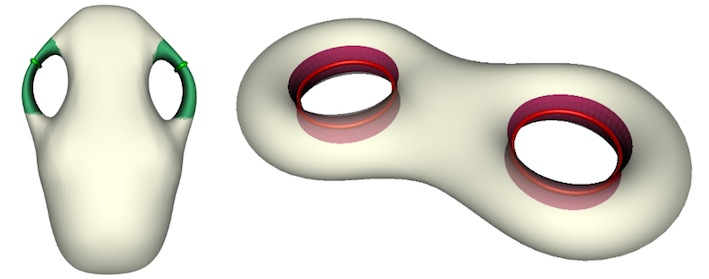
\includegraphics[width=0.66\textwidth]{loop_handle.jpg}
\caption{Handles (green) and tunnels (red) with their defining loops \citep[][]{Dey2012}.}
\label{fig:loop_handle}
\end{figure}\\
A loop defines a handle if it spans a disk in the bounded space bordered by the surface.
If one cuts the surface along such a loop and fills the boundaries with two disks, the handle is eliminated.
Similarly, a tunnel loop spans a disk in the unbounded space bordered by the surface, see figure \ref{fig:loop_handle}.\\
Formalizing this description, let $\mathcal{M}$ be a compact, orientable surface without boundary, i.e. closed and embeddable.
If $\mathcal{M}$ reside inside a $3$-sphere\footnote{ The reason why $\mathcal{M}$ gets embedded in $\mathcal{S}^{3}$, which is a compactification of $\mathbb{R}^{3}$, is to make notations of proofs easier since the space in consideration is finite.}, it separates $\mathcal{S}^{3}$ into two parts $\{(\mathcal{S}^{3} \backslash \mathcal{M})\}$, namely the inside $\mathbb{I}$ and the outside $\mathbb{O}$.
Note that $\mathcal{M}$ is part of both $\mathbb{I}$ and $\mathbb{O}$, analogous to two adjacent triangles that share an edge.
%List \vspace{-2ex}
\begin{itemize}
\setlength{\itemsep}{0cm}
\setlength{\parskip}{0cm}
	\item A tunnel loop is a loop of which the homology class is trivial in $\mathrm{H}^{1}(\mathbb{O})$ and non-trivial in $\mathrm{H}^{1}(\mathbb{I})$.
	\item Accordingly a handle loop has a trivial homology class in $\mathrm{H}^{1}(\mathbb{I})$ and a non-trivial in $\mathrm{H}^{1}(\mathbb{O})$.
\end{itemize}

In other words, handles and tunnels are characterized by the fact that they can be contracted to a point on the inside but are incontractible from the outside and vice versa.
By definition, the set of tunnel loops are disjoint from the set of handle loops, i.e. no handle can be at the same time a tunnel and conversely.
However, not every non-trivial loop on $\mathcal{M}$ is either a handle or a tunnel and both conditions have to be fulfilled, see figure \ref{fig:loop_nontrivial}.

It can be shown shown that for any connected closed surface $\mathcal{M} \subset \mathcal{S}^{3}$ of genus $g$, there exist exactly g handle and tunnel loops: $\{\mathrm{c}^{handle}_{i}, \mathrm{c}^{tunnel}_{i}\}$, with $0 < i \leq g$ forming a basis for $\mathrm{H}(\mathbb{O})$, respectively $\mathrm{H}(\mathbb{I})$.
Furthermore the homology class of circles, that is represented by $[\mathrm{c}^{handle}_{i}]$ and $[\mathrm{c}^{tunnel}_{i}]$ form a basis for $\mathrm{H}^{1}(\mathcal{M})$, which relates them directly to the Betti number $\beta^{1}$, as expected, and will be of great importance in subsection \ref{math_persistence}.\\
The proof involves more algebraic topologic than what was already covered, especially Mayer–Vietoris sequences, therefore we omit the technicalities but instead describe the idea behind it.\\
We saw that $\mathcal{M}$ bisects the space in which it is embedded, $\mathcal{S}^{3} = \mathbb{I} \cup \mathbb{O}$.
Hence it follows that: $\mathrm{H}^{1}(\mathcal{M}) = \mathrm{H}^{1}(\mathbb{I}) \oplus \mathrm{H}^{1}(\mathbb{O})$, with the direct sum of abelian groups.
More importantly it also holds that:
\begin{equation}
rank(\mathrm{H}^{1}(\mathcal{M})) = rank(\mathrm{H}^{1}(\mathbb{I})) + rank(\mathrm{H}^{1}(\mathbb{O})) = 2g
\end{equation}
For symmetry reasons it can be inferred that actually: $rank(\mathrm{H}^{1}(\mathbb{O})) = rank(\mathrm{H}^{1}(\mathbb{I}))$, thus proving that a $2$-manifold of genus g, will always have g tunnel and handle loops.
%Figure
\begin{figure}[htb]
\centering
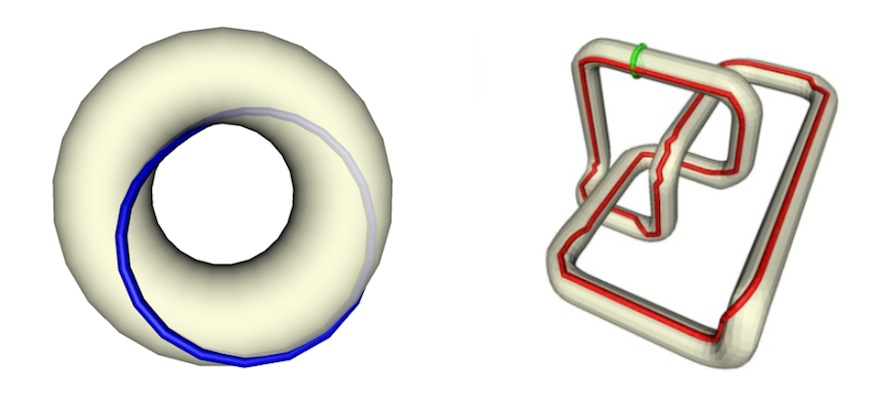
\includegraphics[width=0.66\textwidth]{loop_nontrivial.jpg}
\caption{Left: A non-trivial loop that is neither a handle nor a tunnel, Right: Loops on knotted surface reject the divide in $\mathrm{H}^{1}(\mathbb{I})$ and $\mathrm{H}^{1}(\mathbb{O})$ \citep[][]{Dey2012}.}
\label{fig:loop_nontrivial}
\end{figure}\\
Although this theorem assures the existence of handle and tunnel loops on all connected closed surfaces, they do not bear intuitive meaning on knotted surfaces.
Figure \ref{fig:loop_nontrivial} shows such a surface, which is obtained by thickening a trefoil knot.
Contrary to the natural intuition the red loop is not a tunnel loop.
It is not trivial in $\mathrm{H}^{1}(\mathbb{O})$ yet it can be shown that it generates $\mathrm{H}^{1}(\mathbb{I})$.
This problems can be ameliorated but it introduces unnecessary complexity and consequently we restrict any manifold from here on to be knot free, which is not a problematic restriction in practice.\\

%\newpage
\subsection{Topological Persistence}
\label{math_topological_persistance}

The concept of persistent homology has been introduced, independently by \textit{Robins} \citep[][]{Robins1999} and \textit{Edelsbrunner} \citep[cf.][]{Edelsbrunner2000}.
It provides a mathematical tool, along with a combinatorial algorithm, to capture geometric shapes and is closely related to spectral sequences, mathematical ideas that have been developed 50 years ago\footnote{ See the glossary in \ref{appendix_glossary} and chapter 1.4 of \citep[][]{Zomorodian2005} for more information.}.\\
The main idea behind it, is to study the topological changes of a mesh during an induced growth process and to keep track of how long a topological change lasts, that was induced by a  certain simplex.
This is done by monitoring the homology groups and Betti numbers.\\
In order to measure the longevity of a topological feature, we need two further ingredients, one geometric, assigning a function to a space, the other algebraic, turning the function into measurements.
The measurements make sense, only if the function does, which is studied by substituting an ordering of the simplices for the function\footnote{ This section and its figures are compiled, from the papers: \citep[cf.][]{Delfinado1995}, \citep[cf.][]{Edelsbrunner2000}, \citep[cf.][]{Edelsbrunner2001}, \citep[cf.][]{Zomorodian2008} and \citep[cf.][]{Edelsbrunner2006}. It seems one scholar focused, but not only did \textit{Edelsbrunner} lay the foundations of the field, he is also one of the most highly cited researchers, see: \href{http://researchanalytics.thomsonreuters.com/highlycited/categories/computer_science/}{ISI Highly Cited}. For a complete introduction, a thorough survey of the entire field and the current research, see \citep[][]{Kozlov2008}.}.

\subsubsection{Filtration}
\label{math_filtration}

Let $\mathrm{K}$ be a simplicial complex. A filtration is a nested sequence of subcomplexes and we may think of the filtration as a description of how to construct $\mathrm{K}$ by adding individual parts of it, one after another: $\emptyset = \mathrm{K}_{-1} \subset \mathrm{K}_{0} \subset \mathrm{K}_{1} \subset \dots \subset \mathrm{K}_{n} = \mathrm{K}$\\
More than in the sequence of complexes, we are interested in their topological evolution, expressed by the corresponding sequence of homology groups.
This is possible, since for every $\mathrm{K}_{n-1} \subset \mathrm{K}_{n}$ with $n \geq 1$, the inclusion map induces a homomorphism between the homology groups: $f : \mathrm{H}(\mathrm{K}_{n-1}) \rightarrow \mathrm{H}(\mathrm{K}_{n})$.
Hence, the nested sequence of complexes corresponds to sequences of connected homology groups:
\begin{equation} \label{eq:filtration_persistence}
	0 = \mathrm{H}(\mathrm{K}_{0}) \rightarrow \mathrm{H}(\mathrm{K}_{1}) \rightarrow \dots \rightarrow \mathrm{H}(\mathrm{K}_{n}) = \mathrm{H}^{p}(\mathrm{K})
\end{equation}
Where $p$ represents the homomorphism for each dimension, corresponding to the type of $n$-simplices.
As a consequence the filtration defines a partial ordering on the simplices with: $\sigma_{early} \in (\mathrm{K}_{n-1}-\mathrm{K}_{n})$ preceding $\sigma_{late} \in (\mathrm{K}_{n}-\mathrm{K}_{n+1})$.\\
This total ordering can be extended by deciding on the ordering of the simplices within each $\mathrm{K}_{n-1}-\mathrm{K}_{n}$.
For simplicity one can assume that this ordering consists in the addition of a single simplex at a time.
In other words, the simplices of $\mathrm{K}$ are ordered as $\sigma_{0}, \sigma_{1}, \dots$ such that $\mathrm{K}_{i} = \{\sigma_{0}, \sigma_{1}, \dots, \sigma_{i}\}$, for each $i \leq n$, avoiding ties that result from the otherwise simultaneous creation of simplices, e.g. when a new edge creates a triangle.\\
For example, a $2$-manifold filtration is executed by first adding all the $0$-simplices (vertices) to the set, then including the $1$-simplices (edges) and finally the $2$-simplices (triangle planes), see also figure \ref{fig:filtration_sequence} and the description in the next subsection.

\subsubsection{Incremental Betti Numbers}
\label{math_incremental_betti}

The ordering of simplices in a filtration permits a simple algorithm for computing Betti numbers.
Suppose the sequence of $K_{i} = \{ \sigma_{j} \,|\, 0 \leq j \leq i \}$, for $i \leq n$.
The initial Betti numbers for the set of the empty simplicial complex is obviously $\beta^{0} = \beta^{1} = \beta^{2} = 0$, and the algorithm then works as follows:
%Algorithm
\begin{table}[htb] \bigskip \centering
\setlength{\tabcolsep}{5pt}
\renewcommand{\arraystretch}{1.10}
\fbox{
	\begin{minipage}{10cm}
	\begin{tabular}{l | l} 
			&	\textsc{Betti-numbers ()} \\[1ex]
		\tiny{1}	&	\hspace{0.2cm}	\textsf{for $i=0$ to $n-1$ do} \\
		\tiny{2}	&	\hspace{1.0cm}	\textsf{$k = dim(\sigma_{i}) - 1$} \\
		\tiny{3}	&	\hspace{1.0cm}	\textsf{if $\sigma_{i}$ belongs to a (k+1)-cycle in $\mathrm{K}_{i}$} \\
		\tiny{4}	&	\hspace{1.5cm}	\textsf{then $\beta^{k+1} = \beta^{k+1}+1$} \\
		\tiny{5}	&	\hspace{1.5cm}	\textsf{else $\, \beta^{k} = \beta^{k}-1$} \\
		\tiny{6}	&	\hspace{1.0cm}	\textsf{endif} \\
		\tiny{7}	&	\hspace{0.2cm}	\textsf{endfor} \\
		\tiny{8}	&	\hspace{0.2cm}	\textsf{return $(\beta^{0}, \beta^{1}, \beta^{2})$} \\[1ex] 
	\end{tabular} \end{minipage}
}
	\medskip
	\caption{Algorithm -- Betti numbers of simplicial complexes.}
	\label{algo:betti_numbers}
\end{table}\\
The only question remaining is, how to decide whether a simplex $\sigma_{i}$ belongs to a cycle in $\mathrm{K}_{i}$, or not? 
For vertices $dim(\sigma_{i}) = 0$ it is defined, since every connected vertex belongs automatically to a $0$-cycle\footnote{ We imply that there are no ``free floating'' unconnected vertices allowed in the set $\mathrm{K}$.}.
To decide this for edges, we have to maintain a representation of the connected components, since an edge belongs to a $1$-cycle if and only if its two endpoints belong to the same component, i.e. if it closes a triangle.
Triangles $dim(\sigma_{i})=2$ are treated similarly, checking correspondence with $2$-cycles.\\
This definition sounds rather abstract, but can be easily made clear by showing a filtration.
We call a simplex positive $\Prefix^{+}{\sigma}$, if it belongs to a cycle and negative $\Prefix^{-}{\sigma}$, if it doesn't.
In figure \ref{fig:filtration_sequence}, a filtration is depicted that builds a tetrahedron with a flag.
Each step, shown by the number in the lower left box, adds one simplex to the set $\mathrm{K}_{i}$ with $0 \leq i \leq 17$.
%Figure
\begin{figure}[htb]
\centering
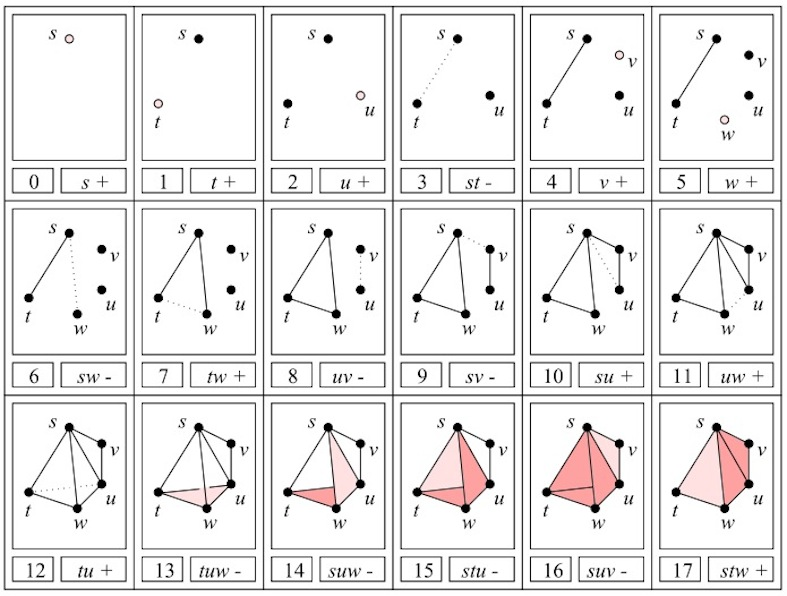
\includegraphics[width=0.75\textwidth]{filtration_sequence.jpg}
\caption{Example of a filtration sequence, building a tetrahedron with flag triangle.}
\label{fig:filtration_sequence}
\end{figure} \vspace{-2ex}
\begin{itemize}
  \setlength{\itemsep}{0cm}%
  \setlength{\parskip}{0cm}%
	\item Vertices $\{s, t, u, v, w\}$ increment $\beta^{0}$ -- steps: $0, 1, 2, 4, 5 ~\longrightarrow~ \beta^{0} = +5$
	\item Edges $\{st, sw, uv, sv\}$ decrement $\beta^{0}$ -- steps: $3, 6, 8, 9 ~\longrightarrow ~\beta^{0} = +5-4$
	\item Edges $\{tw, su, uw, tu\}$ increment $\beta^{1}$ -- steps: $7, 10, 11, 12 ~\longrightarrow ~\beta^{1} = +4$
	\item Faces $\{tuw, suw, stu, suv\}$ decrement $\beta^{1}$ -- steps: $13, 14, 15, 16 ~\longrightarrow ~\beta^{1} = +4-4$
	\item Face $\{stw\}$ increments $\beta^{2}$ -- step: $17 ~\longrightarrow ~\beta^{2} = +1$
\end{itemize}
We can now summarize the incremental steps and get: $\beta^{0} = 1, \,\beta^{1} = 0, \,\beta^{2} = 1$ meaning that there is one component with no non-trivial loops, encapsulating one void.
Also, since $\chi(\mathrm{K}) = \sum_{i} (-1)^{i}\beta^{i} = +1 -0 +1 = 2$, we verify the result with what we already know about compact and orientable $2$-manifolds that have no holes, namely their Euler characteristic of $\chi = 2$.
The correctness of the incremental algorithm implies:
\begin{equation} \label{eq:incremental_betti}
	\beta^{i} = |\Prefix^{+}{\sigma^{i}}|-|\Prefix^{-}{\sigma^{i+1}}| \text{ for } i \geq 0
\end{equation}
In other words, the $i^{th}$-Betti number $\beta^{i}$ is the number of $i$-simplices that create $i$-cycles minus the number of ($i$+1)-simplices that destroy $i$-cycles by creating $i$-boundaries.

\subsubsection{Persistent Homology}
\label{math_persistence}

The idea of persistent homology can be described as a measure that ranks attributes by their lifetime in a filtration.
To asses the persistence for a topological feature in the face of growth, positive and negative simplices are being paired\footnote{ We haven't explicitly discussed the relation between positive and negative simplices and omit a proof, but since every Betti number $\beta^{i} \in \mathbb{N}$, it must follow that for every negative simplex $dim$(i+1) exists a positive simplex $dim(i)$ that it pairs: $|\Prefix^{+}{\sigma^{i}}| \geq |\Prefix^{-}{\sigma^{i+1}}|$. Note that while the pairing depends on the filtration, the number of paired tuples and unpaired positive simplices does not. For a discussion of tracking generating cycles if the simplicial complex or the filtration changes, see \citep[][]{Busaryev2010}.}\label{fn:simplex_relation}.
Although this is only the tip of the iceberg of the theory, for our purposes, the concept of pairing is the only aspect we are interested in\footnote{ Not only can persistent homology be used as an invariant that captures the homological history of an arbitrary space, it also has applications in topological approaches for separating signals from noise and has been utilized in various fields. For example to measure structural changes in membrane fusion, which describe key stages in cellular processes such as virus infections \citep[cf.][]{Kasson2007}.}.\\
Figure \ref{eq:filtration_persistence} visualizes two ways of illustrating the pairing of simplices from the filtration process in figure \ref{fig:filtration_sequence}.
Either with half open intervals $[\Prefix^{+}{\sigma_{i}}, \Prefix^{-}{\sigma_{j}})$, or by the two dimensional representation that spans triangles.
The light triangles represent $0$-cycles, the dark ones $1$-cycles and the area indicates the perseverance of a simplex:
%Figure
\begin{figure}[htb]
\centering
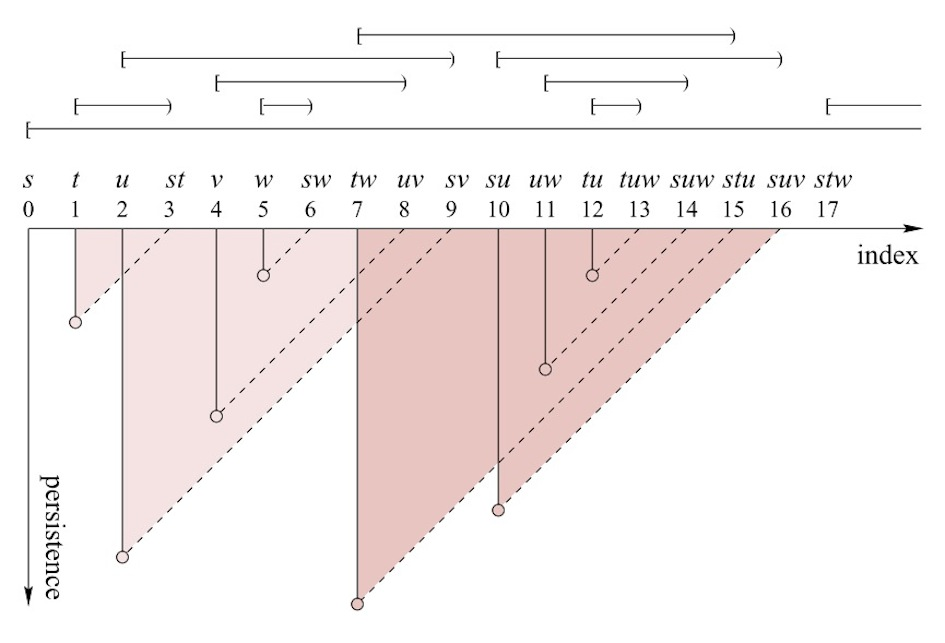
\includegraphics[width=0.60\textwidth]{persistent_homology.jpg}
\caption[Persistence of the simplices]{Persistence of the simplices.}
\label{fig:persistent_homology}
\end{figure}\\
One might note that the vertex $\{s\}$ and the face $\{stw\}$ are unbounded and not drawn.
This is a consequence of equation \eqref{eq:incremental_betti} and means that for every increment of $\beta^{i}$ an unpaired  positive simplex $\Prefix^{+}{\sigma^{i}}$ gets associated that belongs to the homology group of the generating set, i.e the basis.
In other words, each simple connected manifold $\beta^{0} = 1$, has a representative vertex $\sigma^{0}$ and for every non-bounding $1$-cycle, represented by $\beta^{1}$, there is an edge that belongs to a collation of non-contractible closed curves, an so forth.\\
Formally the reasoning behind this observation combines and concludes the work of the entire chapter and will finally explain why we are interested in all of this, as we initially set out to identify certain geometrical features, specifically handles and tunnels.
Combining the relations of $\beta$ as introduced in equations \ref{eq:euler_poincare}, \ref{eq:homology_betti} and \ref{eq:incremental_betti}, we get:
%Equation
\begin{equation} \label{mother_equation}
	\underbrace{ \chi = \sum (-1)^{n} \, \beta^{n}}_{Euler-Poincaré}
	\hspace{3ex} \longrightarrow \hspace{1ex}
	\underbrace{ \beta^{n}}_{n-Betti} =
	\underbrace{ rank ~{Z}^{n} - rank ~\mathrm{B}^{n}}_{Homology~groups} =
	\underbrace{ |\Prefix^{+}{\sigma^{n}}|-|\Prefix^{-}{\sigma^{n+1}}|}_{Filtration}
\end{equation}\\
\underline{Euler-Poincaré:}
Without a question the genus, respectively the Euler characteristic is the most prominent topological invariant.
As intuitive as it might be, it is also very limited in its explanatory reach.
For instance, just judging by $\chi$, there is no way to discriminate whether a tunnel of a manifold was closed or new objects added to the set. 
Therefore we refine the concept with the help of Betti numbers.\\
 \underline{$n$-Betti:} In this way, controlling the topology translates to tinkering with Betti numbers.
Since we are generally not interested in modeling but simplifying the surfaces, we focus on decreasing Betti numbers.
For the most part we deal with just one simple connected manifold, hence $\beta^{0} = 1$ is unchangeable and of minor importance.
Neither is the amount of enclosed voids, denoted by $\beta^{2}$, as it pertains to the characteristics of the interior.
Surfaces do not have $\beta^{i} \neq 0$ with $i \geq 3$, so by exclusion the only really importance falls onto $\beta^{1}$, describing the amount of disjoint non-contractible circles.\\
 \underline{Homology groups:} The integer that represents $\beta^{1}$ actually represents an entire group of circles that belong to the same homologic group.
Consequently we have to expand the concept as we did with the genus that was refined into the Euler-Poincaré formula.
This is achieved by examining the relation of chains in general and specifically the subgroup of chains that bind cycles\footnote{ Hinted by the fact that we introduced $ranks, kernels$ and $images$, it is not surprising that persistence can also be nicely explained in terms of matrix operations, which is a field of study in itself \citep[see chapters IV-3 and VI-1 in][]{Edelsbrunner2006}.}, also see figure \ref{fig:chain_complex}.\\
\underline{Filtration:} The final step is finding one representative circle from the entire homologic group.
To narrow down the selection, we use filtration, as it identifies edges that are boundaries for the circles in question.
That is to say, that after all the mathematical machinery that was put into motion we have firmly proven that for every tunnel or handle of a manifold we can compute an edge that is part of the defining loop.
What is left now, is an exact description of these loops and the algorithm, given in section \ref{math_loop_definition} and \ref{math_loop_computation}.

\subsection{Computing Geometry-aware Loops}
\label{math_loop_computation}

At the end of the last subsection we concluded that if we pair simplices during a filtration, we acquire a set $\mathbb{U} = \{ \Prefix^{+}{\sigma}\}$ of unpaired positive simplices.
We are interested in the subset of simplices $\Prefix^{+}{\sigma^{p}}$ of dimension $p = 1$: $\,\mathbb{U}^{1} \subset \mathbb{U}$  with $|\mathbb{U}^{1}| = 2g$, as this subset consists of edges that represent the tunnel and handle loops of the surface.\\
We now describe the principal steps\footnote{ The following algorithms were first described and proven in \citep[][]{Dey2007} and later refined and sped-up in \citep[][]{Dey2008, Dey2009}. Basically we follow the ideas for pairing simplices, but deviate in the latter stages when optimizing the found loops.} necessary to generate this set and afterwards discuss the two building algorithms in more detailed in subsection \ref{math_algorithm_pairing} and \ref{math_algorithm_looprefinement}.\\
%List
\vspace*{-1.0cm}
\begin{enumerate}
\setlength{\itemsep}{0cm}
\setlength{\parskip}{0.15cm}
\item The input is a simplicial complex $\mathrm{K}_{S}$ that constitutes a closed, orientable surface $\mathcal{M}$. By using a Delaunay meshing algorithm\footnote{ We used the freely available implementation named \href{http://tetgen.berlios.de/}{TetGen} for that purpose \citep[cf.][]{Si2010}.}, one obtains the tessellated convex hull of $\mathcal{M}$, i.e. the simplicial representations for the inside $\mathrm{K}_{\mathbb{I}}$ and the outside $\mathrm{K}_{\mathbb{O}}$, that together form $\mathrm{K} = \mathrm{K}_{S} \cup \mathrm{K}_{\mathbb{I}} \cup \mathrm{K}_{\mathbb{O}}$. Although we are only interested in the circles on $\mathrm{K}_{S}$, we need triangles for the inside and the outside in order to add them to our filtration and find not only unpaired edges but also their corresponding loops.
\item The simplices of the surface $\mathrm{K}_{S}$ are added to filtration in an arbitrary order. Paring each of them with the algorithm described in \ref{math_algorithm_pairing}, gives $2g$ unpaired edges $\mathbb{U}^{1}$.
\item The simplices of $\mathrm{K}_{\mathbb{I}}$ are added to the filtration. Which pairs half of the edges in $\mathbb{U}^{1}$ with negative triangles $\Prefix^{-}{\sigma_{i}^{2}}$ and associates an explicit circle to each edge, i.e. the one that got killed by $\Prefix^{-}{\sigma_{i}^{2}}$, which by definition is a handle loop. The filtration with $\mathrm{K}_{\mathbb{I}}$ can be stopped as soon as $g$ edges of $\mathbb{U}^{1}$ are paired with their circles $\{c^{1}_{handle~i}\}^{g}_{i=1}$, see figure \ref{fig:unpaired-edges_paired-loops} illustrating the steps 2-4.
\item Lastly the simplices of $\mathrm{K}_{\mathbb{O}}$ are included into the filtration. The remaining positive edges in $\mathbb{U}^{1}$ get paired as before, thereby obtaining $g$ more circles that are by definition tunnel loops $\{c^{1}_{tunnel~i}\}^{g}_{i=1}$. Note that loops that get killed by negative triangles in $\mathrm{K}_{\mathbb{I}}$ or $\mathrm{K}_{\mathbb{O}}$ have all their edges lying on $\mathrm{K}_{S}$ because the simplices of the inside and outside only get added after all simplices of $\mathrm{K}_{S}$ are in the filtration.
\item The computed loops are undoubtedly correct as far as homology is concerned, but as can be seen in figure \ref{fig:unpaired-edges_paired-loops}, they are not necessarily appealing in a geometrical sense. For that reason we refine the loops as described in \ref{math_algorithm_looprefinement}.
\end{enumerate}
%Figure
\begin{figure}[htb]
\centering
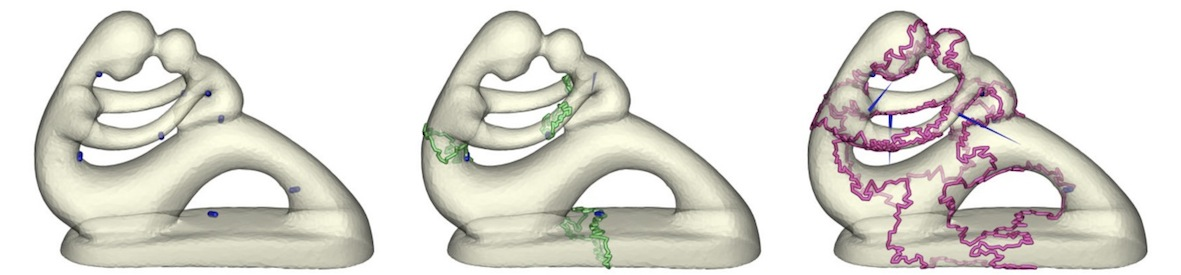
\includegraphics[width=1.0\textwidth]{unpaired-edges_paired-loops.jpg}
\caption{Left to right: Unpaired edges,handle loops and tunnel loops \citep[][]{Dey2012}.}
\label{fig:unpaired-edges_paired-loops}
\bigskip
\end{figure}

\subsubsection{Pairing Algorithm}
\label{math_algorithm_pairing}

Pairing is the essential concept of persistent homology, as it determines the lifetime, i.e. persistence of $n$-cycles.
In order to pair the simplices, we have to determine whether they are negative or positive.
Recall that a simplex $\sigma^{n}$ of dimension $n$, is positive $\Prefix^{+}{\sigma^{n}}$, if it creates a non-bounding $n$-cycle and that it is negative $\Prefix^{-}{\sigma^{p}}$, if it kills an existing ($n$-1)-cycle.
In other words, every new edge $\sigma^{1}$ kills a $0$-cycle, unless it closes a chain $\mathrm{c} = \{ \sigma^{1}_{0}, \sigma^{1}_{1}, \dots , \sigma^{1}_{i} \}$ so that $\partial (\mathrm{c} + \sigma^{1}) = \emptyset$.
In the exemplary case shown in figure \ref{fig:filtration_sequence}, it is not hard to figure the sign out $\Prefix^{\pm}{\sigma}$, but for an arbitrarily large simplicial complex $K$, we need a more elaborate approach using the notion of temporality -- introduced as a consequence of equation \eqref{eq:filtration_persistence}, we defined that for every step in a filtration, exactly one additional simplex gets added with that the latest addition being the youngest simplex of the complex.
Generally speaking $\sigma_{j} = \mathrm{K}_{j} - \mathrm{K}_{j-1}$ is younger than $\sigma_{i} = \mathrm{K}_{i} - \mathrm{K}_{i-1}$, if it appears later in the filtration, i.e. $\mathrm{K}_{j} \supset \mathrm{K}_{i}$.

We analyze parts of the filtration from example \ref{fig:filtration_sequence} to see how the algorithm works before we give a formal description in \ref{algo:simplex_pairing}.\\
In the stage $\mathrm{K}_{3}$ of the process the first edge gets added, before that only the vertices $\sigma^{0}_{0}$ up to $\sigma^{0}_{2}$ populate the simplicial complex. 
All vertices are trivially positive, as there are no ($p$-1)-cycles that could be closed.
This can be shown formally: $\partial \sigma^{0} = \partial \{v\} = \emptyset \,\rightarrow \,\Prefix^{+}{\sigma^{0}}$, since the boundary operator, applied to any vertex, results in the empty set.
Now to pair the new edge $\sigma^{1}_{3} = \{s,t\}$, we check its boundary: $c = \partial \sigma^{1}_{3} = \partial \{s,t\} = (s+t)$.
No circle was closed, which would have left the the boundary empty, thus must be negative and we can pair the simplex with the youngest candidate.
By convention we always assign the youngest unpaired positive simplex to the pair, in this case this is vertex $t$ as it is younger than $s$: $\sigma^{0}_{1} > \sigma^{0}_{0}$ and we get the pairing: $\langle t, st \rangle = \langle \Prefix^{+}{\sigma^{0}_{1}}, \Prefix^{-}{\sigma^{1}_{3}} \rangle$, which is visualized as the first triangle in figure \ref{fig:persistent_homology}.
Now we look at step $\mathrm{K}_{7}$ that introduces the edge $\sigma^{1}_{7}$, that closes a triangle.
More precisely: $c = \partial \sigma^{1}_{7} = \partial \{t, w\} = (t + w)$, but since $t$ and $w$ are already paired, we have to add their pairs respectively their boundaries: $(t + w) = (t + \{s,t\} + w + \{s,w\}) \rightarrow (t + \partial \{s,t\} + w + \partial \{s,w\}) = (t + s + t + w + s + w) = (2s + 2t +2w)$, note that we defined the addition modulo 2: $(2s + 2t +2w) = \emptyset \rightarrow \Prefix^{+}{\sigma^{1}_{7}}$, meaning that the edge is positive.
Generalizing this for the entire simplicial complex, gives us the pairing algorithm:
%Algorithm
\begin{table}[htb] \medskip \centering
\setlength{\tabcolsep}{5pt}
\renewcommand{\arraystretch}{1.2}
\fbox{
	\begin{minipage}{10cm}
	\begin{tabular}{r | l} 
			&	\textsc{Pairing ($\sigma$)} \\[1ex]
		\tiny{1}	&	\hspace{0.2cm}	\textsf{$\mathrm{c} = \partial \sigma^{p} = \{ \sigma_{i}^{p-1}, \dots , \sigma_{j}^{p-1}  \}$} \\
		\tiny{2}	&	\hspace{0.2cm}	\textsf{let $\sigma_{last}$ be the youngest ($p$-1)-simplex in $\mathrm{c}$} \\
		\tiny{3}	&	\hspace{0.2cm}	\textsf{while $\sigma_{last}$ is paired and $\mathrm{c} \neq \emptyset$ do} \\
		\tiny{4}	&	\hspace{1.0cm}	\textsf{let $c_{kill}$ be the cycle which was killed by $\sigma_{last}$} \\
		\tiny{5}	&	\hspace{1.0cm}	\textsf{$c = c + c_{kill}$} \\
		\tiny{6}	&	\hspace{1.0cm}	\textsf{update $\sigma_{last}$ to the youngest ($p$-1)-simplex in $c$} \\
		\tiny{7}	&	\hspace{0.2cm}	\textsf{end while} \\
		\tiny{8}	&	\hspace{0.2cm}	\textsf{if $c \neq \emptyset$ then} \\
		\tiny{9}	&	\hspace{1.0cm}	\textsf{the simplex is negative $\Prefix^{-}{\sigma}$, killing $c$} \\		
		\tiny{10}	&	\hspace{1.0cm}	\textsf{pair $(\sigma_{last}, \Prefix^{-}{\sigma})$} \\
		\tiny{11}	&	\hspace{1.0cm}	\textsf{associate $c$ as $c_{kill}$ with the simplex $(c_{kill}, \Prefix^{-}{\sigma})$} \\
		\tiny{12}	&	\hspace{0.2cm}	\textsf{else} \\
		\tiny{13}	&	\hspace{1.0cm}	\textsf{the simplex is positive $\Prefix^{+}{\sigma}$} \\
		\tiny{14}	&	\hspace{0.2cm}	\textsf{end if} \\[1ex]
	\end{tabular} \end{minipage}
}
	\medskip
	\caption{Algorithm -- Simplex pairing.}
	\label{algo:simplex_pairing}
\end{table}\\
The algorithms spends most of its time expanding $c = \partial \sigma$ in order to decide whether at the end it is empty or not.
We can speed the process up by introducing another condition for the \textsf{while} loop.
It relies on the observation that, at no time during the expansion of $c$, the youngest simplex in $c$ can be older than the oldest simplex in $\mathbb{U}^{1}$, without it automatically being a positive simplex.
This means that if $\sigma_{last} < \Prefix^{+}{\sigma_{last\,\mathbb{U}}} \,\rightarrow \, \Prefix^{+}{\sigma_{last}}$.
The comparison is easy to do, as we only have to check the indices $j$ and $i$ of the corresponding stage of the filtration: $\sigma_{last} = \mathrm{K}_{j} - \mathrm{K}_{j-1}$ and $\Prefix^{+}{\sigma_{last\,\mathbb{U}}} = \mathrm{K}_{i} - \mathrm{K}_{i-1}$.\\
The observation can be formally proven but it is explicitly clear, considering the fact that after the filtration of $\mathrm{K}_{\mathcal{S}}$, only positive simplices are unpaired and that it is not possible to be left with unpaired negative simplices at that point\footnote{ See the first footnote on page \pageref{fn:simplex_relation} for more explanation.}.

\subsubsection{Refining the Loops}
\label{math_algorithm_looprefinement}

After the entirety of this chapter we are now finally at the point where we actually have the loops representing the topological features we wanted to find, namely handles and tunnels.
To be precise, we have a number of homologous circles that we acquire in the \textsf{while} loop of algorithm \ref{algo:simplex_pairing}.
During the process of finding the paired positive edges for a negative triangle we get a series of them and now have to choose one among them.

The previous work of \citep[][]{Dey2007, Dey2008, Dey2009} has devoted considerable effort to perfect the selection by two methods: 
One is to assign geodesic sizes to the triangles in $\mathrm{K}_{\mathbb{I}}$ and $\mathrm{K}_{\mathbb{O}}$, respectively the projection of their edges onto the surface.
This is done to then order them according to size and introduce them, smallest triangle first to the filtration, thereby ensuring to pair smaller loops first.
The other method drops the idea to connect the handle and tunnel loops to their unpaired positive edges all together.
Instead the shortest circle in the homology class is searched, broadening the search immensely.
%Figure
\begin{figure}[htb]
\centering
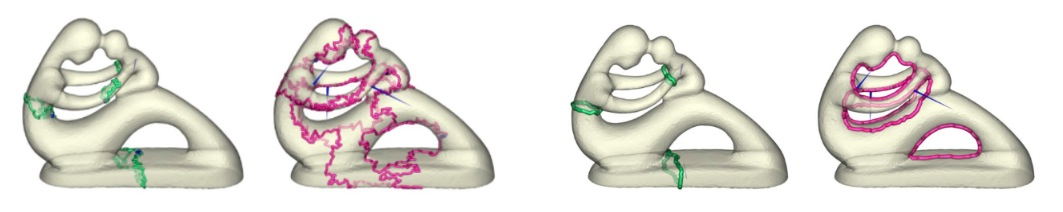
\includegraphics[width=1.0\textwidth]{loop_refinement.jpg}
\caption{Initial results and refined loops on the right \citep[][]{Dey2009}.}
\label{fig:loop_refinement}
\end{figure}\\
These two refinements undoubtedly improve the geometrical appearance greatly, as seen in figure \ref{fig:loop_refinement}.
However we find the prize in computational expenses to be too high.\\
The only costly stage in the entire sequence thus far has been the Delaunay triangulation, which we consider to be a pre-process that can be automated and done in advance.
One advantage of the persistence based algorithm is that it is combinatorial in nature and thereby avoids costly, error-prone numerical computations.
Unlike many previous methods, the algorithm does not require computing any extra data structures such as Reeb graphs, medial axes, or curve skeletons\footnote{ In 2D, the medial axis of a shape is a set of curves defined as the locus of points that have at least two closest points on the boundary of the shape. In 3D, the corresponding object is also called the medial surface because in addition to curves, it can contain surface patches.\\
Likewise a curve skeleton is an abstract 1D geometrical representation of 3D shapes that considers topological features. By segmenting the object it can help spatial understanding, providing a higher level description of the object.}.
We find it of pivotal importance to try and keep the workflow as fast as possible, not changing workflow regime.
As mentioned in section \ref{introduction4}, we firmly believe that interactivity trumps automation and legitimates then necessary user interaction to obtain similar results.\\
Accordingly our solution for refining the computer loops is to substitute the geodesic metric by a simple edge-count.
This is reasonable given the fact that for most triangle surfaces the edge size does not vary much in local neighborhoods.
To further improve the results we give the user the freedom to manually tweak circles be changing parts of the path.
Not only does this ameliorate the quality chasm between the reference implementation and our solution but also lends itself nicely to the simplification step where the user defines which loops to kill by triangulating them, see section \ref{topstoc0} for the details.

This concludes this chapter \ref{math0}, we have talked about basic topology in section \ref{math1}, as well as more advanced concepts like filtration in section \ref{math2} and found a way to leverage the theory to describe and find topological features.
Having described the algorithms involved we now turn to the actual application of the techniques.
We will discuss in the next chapter \ref{topstoc0}, among other principles, how to put them use.
Resulting in a direct and useful workflow to simplify not only fast and robustly, but also with numerous levers that can be tweaked directly by the user -- one being the control over topology.

% smiley command: $\ddot\smile$

\chapter{User-Guided Mesh Simplification}
\label{topstoc0}

\begin{flushright}
\textit{``The original motivation to do research [that led to technological discoveries]\\was to expand the range of possibilities for storytellers.''}\\
-- Ed Catmull {[}at the 73rd Scientific and Technical Academy Awards, 2001{]}
\end{flushright}

In this section we finally want to connect the theoretical part with the practical application.
We will illustrate the workings of our reference implementation\footnote{ Our reference implementation was written in STL conform \texttt{C++}. The only dependancies are \href{http://www.openmesh.org/}{OpenMesh} which provides the data structure for the mesh operations, \href{http://www.qtcentre.org/content/}{Qt} for the \texttt{GUI} and \href{http://www.libqglviewer.com/}{libQGLViewer} that facilitates the incorporation of \texttt{OpenGL} for the view-port. Although the core algorithms are very lean, the entire code-basis has grown to well over 4000 lines of code over the course of the thesis.
Right now, most parts are not appropriately documented, but after some annotations are added, it will be made available -- feel free to inquire via \href{mailto:mail@lnpe.at}{mail@lnpe.at}.} and discuss our results.\\
First, we will briefly describe the so called ``TopStoc'' algorithm in section \ref{topstoc1}.
It serves as the core decimation method to which the other tools were added.
The following three subsections \ref{topstoc121}, \ref{topstoc122} and \ref{topstoc123}, discuss three useful adaptations of ``TopStoc'' that we made use of.

The next section \ref{topstoc2} then lays out the topological options for the user.
\ref{topstoc21} shows what type of information the user gets and how it is presented to her.
For instance, open boundaries get treated much like handle or tunnel loops, as they are also topologically important circles.
Besides the tools to change the topology, described in \ref{topstoc22}, we will also talk about the limitations of our approach in \ref{topstoc23}.

The rest of the chapter from section \ref{topstoc3} to \ref{topstoc43} then illustrates further ways of valuable user-interaction and how to leverage guidance as well as practical considerations like support for textures in \ref{topstoc42}.
Last but not least, we will come to talk about how to measure and evaluate results of any decimation and the two principe ways \ref{topstoc51} and \ref{topstoc52}, we found most suitable to work with.


\section{The TopStoc Algorithm}
\label{topstoc1}

The basis for our work are the two algorithms described in the paper ``Stochastic Sampling and Topological Clustering'' \citep[cf.][]{Boubekeur2009}.
The main advantage over other solutions, undoubtedly is its speed, typically surpassing the quasi decimation standard ``QSlim'' by an order of magnitude.
Consequently it is a natural fit for any system that wants to offer smooth interaction for user-guidance. 
%Bild
\begin{figure}[ht]
\centering
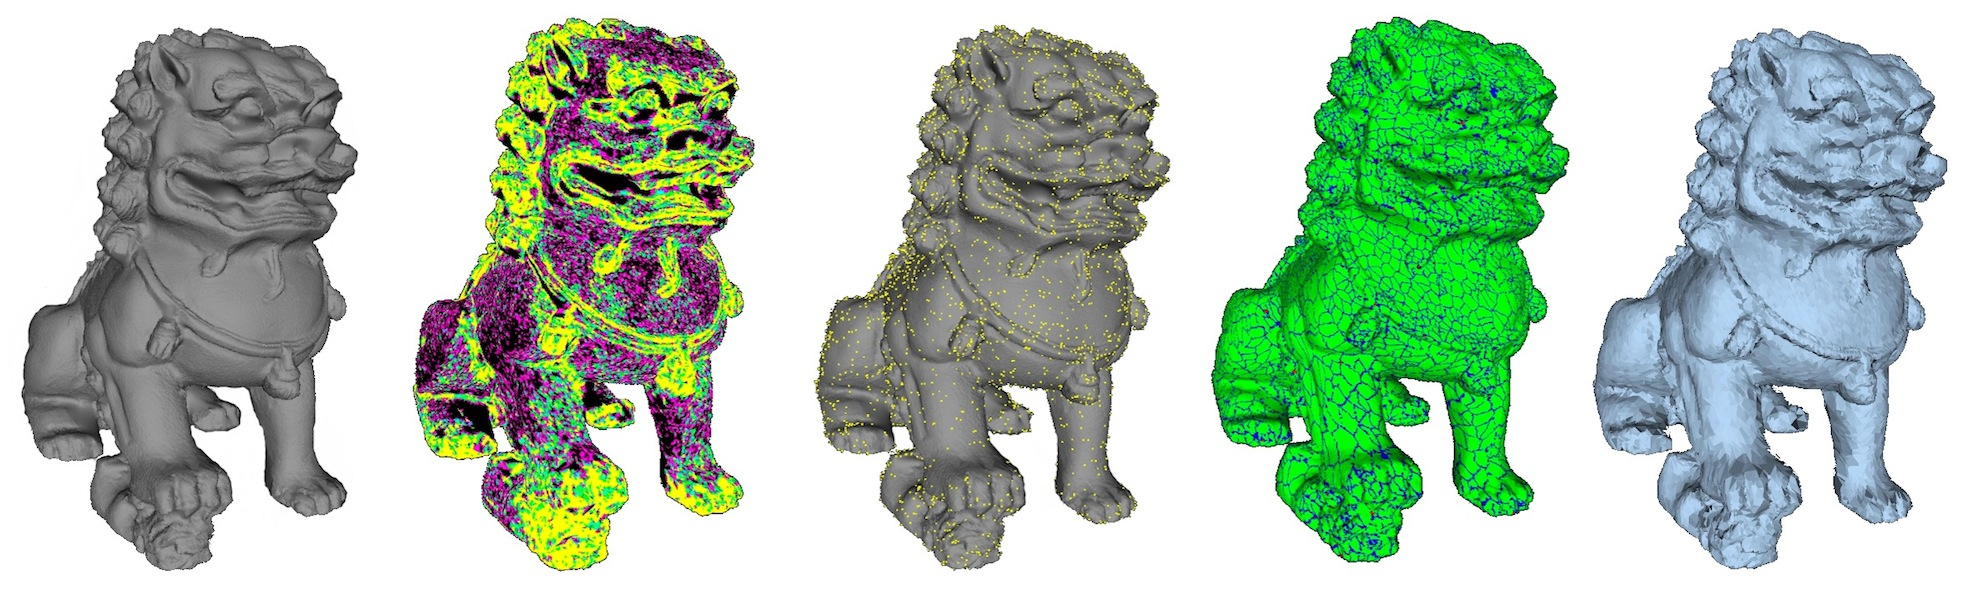
\includegraphics[width=1.0\textwidth]{topstoc_dragons.jpg}
\caption{Results from our TopStoc implementation, left to right: The base mesh; visualization of the local normal deviation; sampled vertices that define the low-resolution mesh; visualization of the topological clustering; the final mesh.}
\label{fig:topstoc_dragons}
\end{figure}\\
Before we can treat any modifications we give an 'as short as possible' rundown of the individual steps, as laid out in the original paper:
%\vspace{-2ex}
\begin{itemize}
%\setlength{\itemsep}{0cm} \setlength{\parskip}{0cm}
	\item \textit{Stochastic Vertex Selection} -- to select the ``best'' vertices for a low resolution model, every vertex is assigned a value $\mathrm{x}$ of geometric importance, we refer to as weight: \begin{equation} \label{eq:vertex_weight}
\mathrm{x}(\mathrm{v}) \,=\, \frac{|\mathrm{N}_{v}| - \sum_{\mathrm{u} \in \mathrm{N}_{v} } (\textbf{n}^{T}_{v}\textbf{n}_{u})}{2 \cdot |\mathrm{N}_{v}|}
\end{equation}
In other words, for every vertex the normal deviation of its immediate surroundings, i.e. the so called one-ring of vertex normals is calculated. Depending on the weight of each vertex and the target size, a subsample is selected. Note that the probability distribution must be tweaked, so that subsampling in flat areas is avoided. The second and third dragon in figure \ref{fig:topstoc_dragons} show the vertex weight and an example of sampled vertices.
	\item \textit{Topological Clustering} -- the sampled vertices are used to partition the mesh via a breadth-first flood-filling. This way every vertex of the base mesh is allotted to one representative. Following the idea of vertex clustering each of the sub-meshes is used to retriangulate the surface, but instead of spatial distance, the topological proximity defines the grid cells. Thus, contrary to normal clustering, the homotopy between the base and the decimated mesh can be ensured. The penultimate dragon in figure \ref{fig:topstoc_dragons} shows the result of a flood-filling. Green areas mark topological cells, blue triangles the border between any two of them and red faces indicate an intersection of three different cells that determine the connectivity of the new mesh.
	\item \textit{Density Control} -- not part of the basic decimation suit, rather an option, is this method a way to improve the shapes of the resulting triangles. There are already many concepts to refine triangles, but most of them are very costly. Density control avoids this relapse to high complexity by using a strategy inspired by ``Poisson disk rejection sampling''. Before the sampled vertices are used in the topological cluster stage, each neighborhood of a sampled vertex gets rid of other samplings within a given distance. 
\end{itemize}


\subsection{Fast Topological Clustering}
\label{topstoc121}

As already mentioned, the stochastic vertex selection as well as the topological clustering are both very fast.
However, of these two, the latter is considerably slower than the first.
Not only is the clustering more algorithmically complex, but also is there no immediate way to quickly accelerate it.
The calculation of weights and the selection of vertices can be trivially sped up by implementing a parallelized version of the algorithm, as every individual decision is completely independent of the other calculations\footnote{ Given that every SIMD threat has access, not only to one vertex, but also the adjacent vertices.}.
For this reason we are more interested in improving the clustering stage and propose a small modification that pays of for cases in which the target sizes is very small, i.e. below ca. 5\%.

The algorithm in its original version only needs the set of sampled vertices $\overline{\mathcal{V}}$ and a queue $\mathrm{Q}$ to store vertex references, besides the means to navigate the neighborhood of any vertex on the surface of course.
During the flood-fill every vertex of the base mesh gets touched once to assign the mark of the cell it belongs to, see algorithm \ref{algo:topological_clustering}.
Only to then iterate one more time over the entire mesh to check whether three different cell marks coincide on a given face.
%Algorithm
\begin{table}[htb] \medskip \centering
\setlength{\tabcolsep}{5pt}
\renewcommand{\arraystretch}{1.10}
\fbox{
	\begin{minipage}{10cm}
	\begin{tabular}{r | l} 
				&	\textsc{Breadth-first flood-filling ($\overline{\mathcal{V}}$)} \\[1ex]
		\tiny{1}	&	\hspace{0.2cm}	\textsf{for each vertex $\mathrm{v}$ in $\overline{\mathcal{V}}$ do} \\
		\tiny{2}	&	\hspace{1.0cm}	\textsf{mark $\mathrm{v}$ with $\mathrm{v}$} \\
		\tiny{3}	&	\hspace{1.0cm}	\textsf{append reference of $\mathrm{v}$ to $\mathrm{Q}$} \\
		\tiny{4}	&	\hspace{0.2cm}	\textsf{end for} \\
		\tiny{5}	&	\hspace{0.2cm}	\textsf{while $\mathrm{Q}$ is not empty do} \\
		\tiny{6}	&	\hspace{1.0cm}	\textsf{$\mathrm{v} :=$ head of $\mathrm{Q}$} \\
		\tiny{7}	&	\hspace{1.0cm}	\textsf{for each vertex $\mathrm{u}$ in $\mathrm{N}_{V}[\mathrm{v}]$ do} \\
		\tiny{8}	&	\hspace{1.6cm}	\textsf{if $\mathrm{u}$ is not marked then} \\		
		\tiny{9}	&	\hspace{2.0cm}	\textsf{mark $\mathrm{u}$ with mark of $\mathrm{v}$} \\
		\tiny{10}	&	\hspace{2.0cm}	\textsf{append $\mathrm{u}$ to $\mathrm{Q}$} \\
		\tiny{+11}&	\hspace{1.6cm}	\textsf{else if mark is different to $\mathrm{v}$ then} \\
		\tiny{+12}&	\hspace{2.0cm}	\textsf{append the associated face $\mathrm{f}_{\mathrm{u}}$ to $\mathrm{L}$} \\
		\tiny{13}	&	\hspace{1.6cm}	\textsf{end if} \\
		\tiny{14}	&	\hspace{1.0cm}	\textsf{end for} \\
		\tiny{15}	&	\hspace{1.0cm}	\textsf{pop head of $\mathrm{Q}$} \\
		\tiny{16}	&	\hspace{0.2cm}	\textsf{end while} \\[1ex]
	\end{tabular} \end{minipage}
}
	\medskip
	\caption{Algorithm -- Breadth-first flood-filling.}
	\label{algo:topological_clustering}
\end{table}\\
In the modified version, we use knowledge about the connectivity of the decimated mesh to discard faces early on that can not qualify as candidates later.
%We check whether the mark of vertex $\mathrm{v}$, with which another vertex $\mathrm{u}$ should have been marked are identical.
In the case that vertex $\mathrm{u}$ can't be marked by $\mathrm{v}$ because it was previously marked, there are two scenarios:
Either it was already marked by $\mathrm{v}$ during an earlier step of the flood-fill, or it was marked by a different vertex $\mathrm{s}$.
Note that in the end, what we are ultimately interested in, is finding only the faces where all three vertices were marked by separate vertices.
Hence, if vertex $\mathrm{v}$ encounters an already marked vertex $\mathrm{u}$ that bears the same mark as itself, it is impossible for the two adjacent faces -- of the edge connecting $\mathrm{v}$ and $\mathrm{u}$ -- to be one of these interesting faces.\\
Understanding this, we append faces to an unique list $\mathrm{L}$, i.e. without allowing multiple entries, if during the flood-fill two different marks where found.
The new steps in the algorithm are marked with '$+$' in \ref{algo:topological_clustering}.
Note that we only add one face $\mathrm{f}_{u}$ to $\mathrm{L}$, not both, this is because the check will happen two times from both sides starting with either vertex once.
For an improved runtime it is important to avoid multiple insertions, consistently attaching either the face of the outgoing or the incoming half-edge only.

%Bild
\begin{figure}[hbt]
\centering
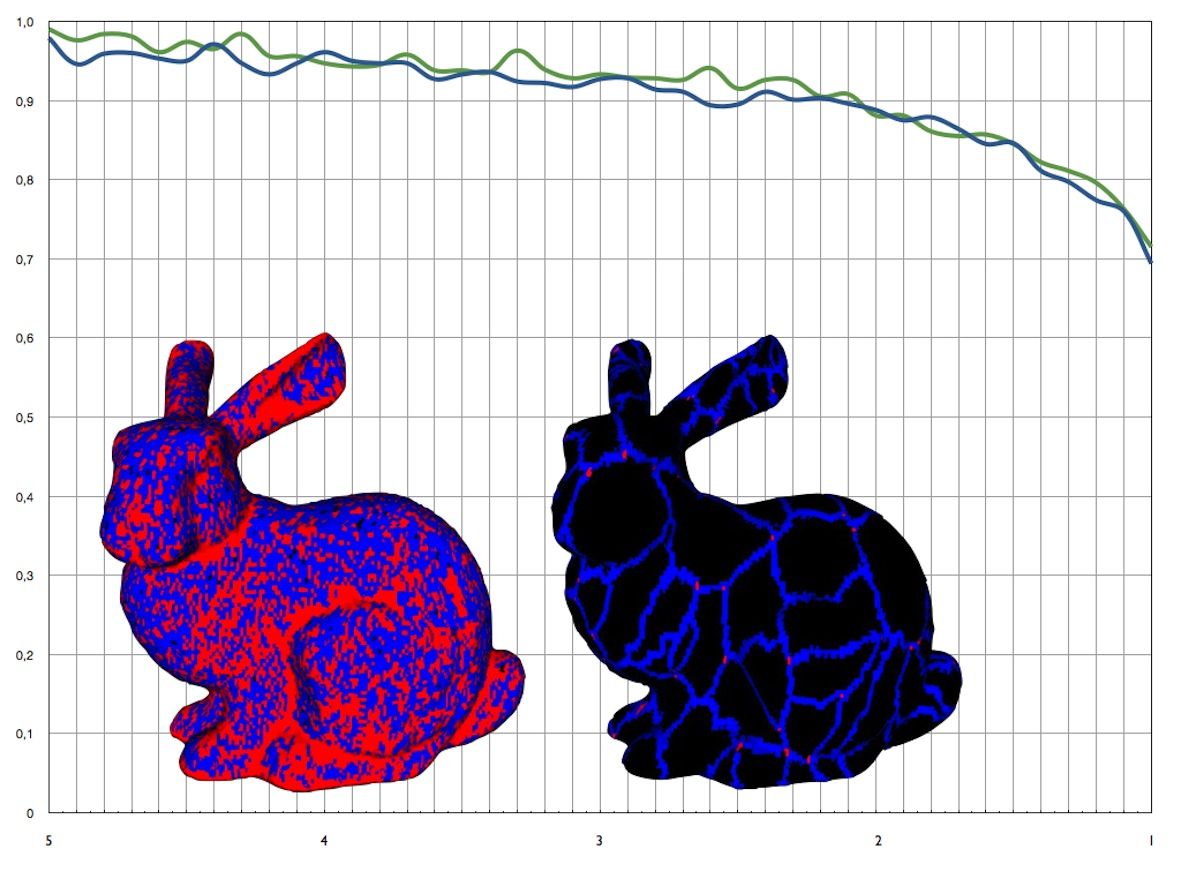
\includegraphics[width=1.0\textwidth]{fast_clustering.jpg}
\caption{The Y-axsis shows the relative improvement in \% of the runtime for two models (green/blue), for decimation ratios between 5\% and 1\% on the X-axis. To demonstrate the effect, the two bunnies show the discarded faces in black, for a very high and a very low sampling.}
\label{fig:fast_clustering}
\end{figure}
Although the final list of faces to check holds far less references, a speed-up manifest itself only for high decimation rates.
This is due to the fact that inserting faces to the list $\mathrm{L}$ is very costly.\\
For example, decimating the \textit{Chinese Dragon} Model, from initially over 655,000 vertices to about 3\%, the runtime decreased at about 8\%.
For target sizes around 1\% the speed-ups can be far greater, succeeding 30\%.
In figure \ref{fig:fast_clustering} we plotted the relative runtime $\frac{t_{fast}}{t_{normal}}$ for two models, namely the \textit{Stanford Bunny} in green and the \textit{Chinese Dragon} in blue\footnote{ Each measurement was taken multiple times in 0.1\% steps for the interval of 5\% down to 1\%.}.\\
As the target size is known before the flood-fill occurs, we automatically use this feature in case the the target size is smaller than 5\%\,\footnote{ Note that ``TopStoc'' in general is better suited for high decimation ratios, as it is especially advantages over other solutions in these cases.}.

\newpage
\subsection{Adaptive Density Control}
\label{topstoc122}

Density control as introduced in the original paper can greatly improve the quality of decimated mesh triangulation.
Having said that, it suffers two drawbacks. 
$\epsilon$ defines the minimum distance between two sampled vertices, as $\epsilon$ increases the resulting mesh resembles more and more what one would expect from a uniform sampling. 
Thereby negating the intention and design of the the stochastic selection phase of the vertices.
The second problem is that the clean-up process can increase the runtime noticeably, up to 50\%.
%Bild
\begin{figure}[ht]
\centering
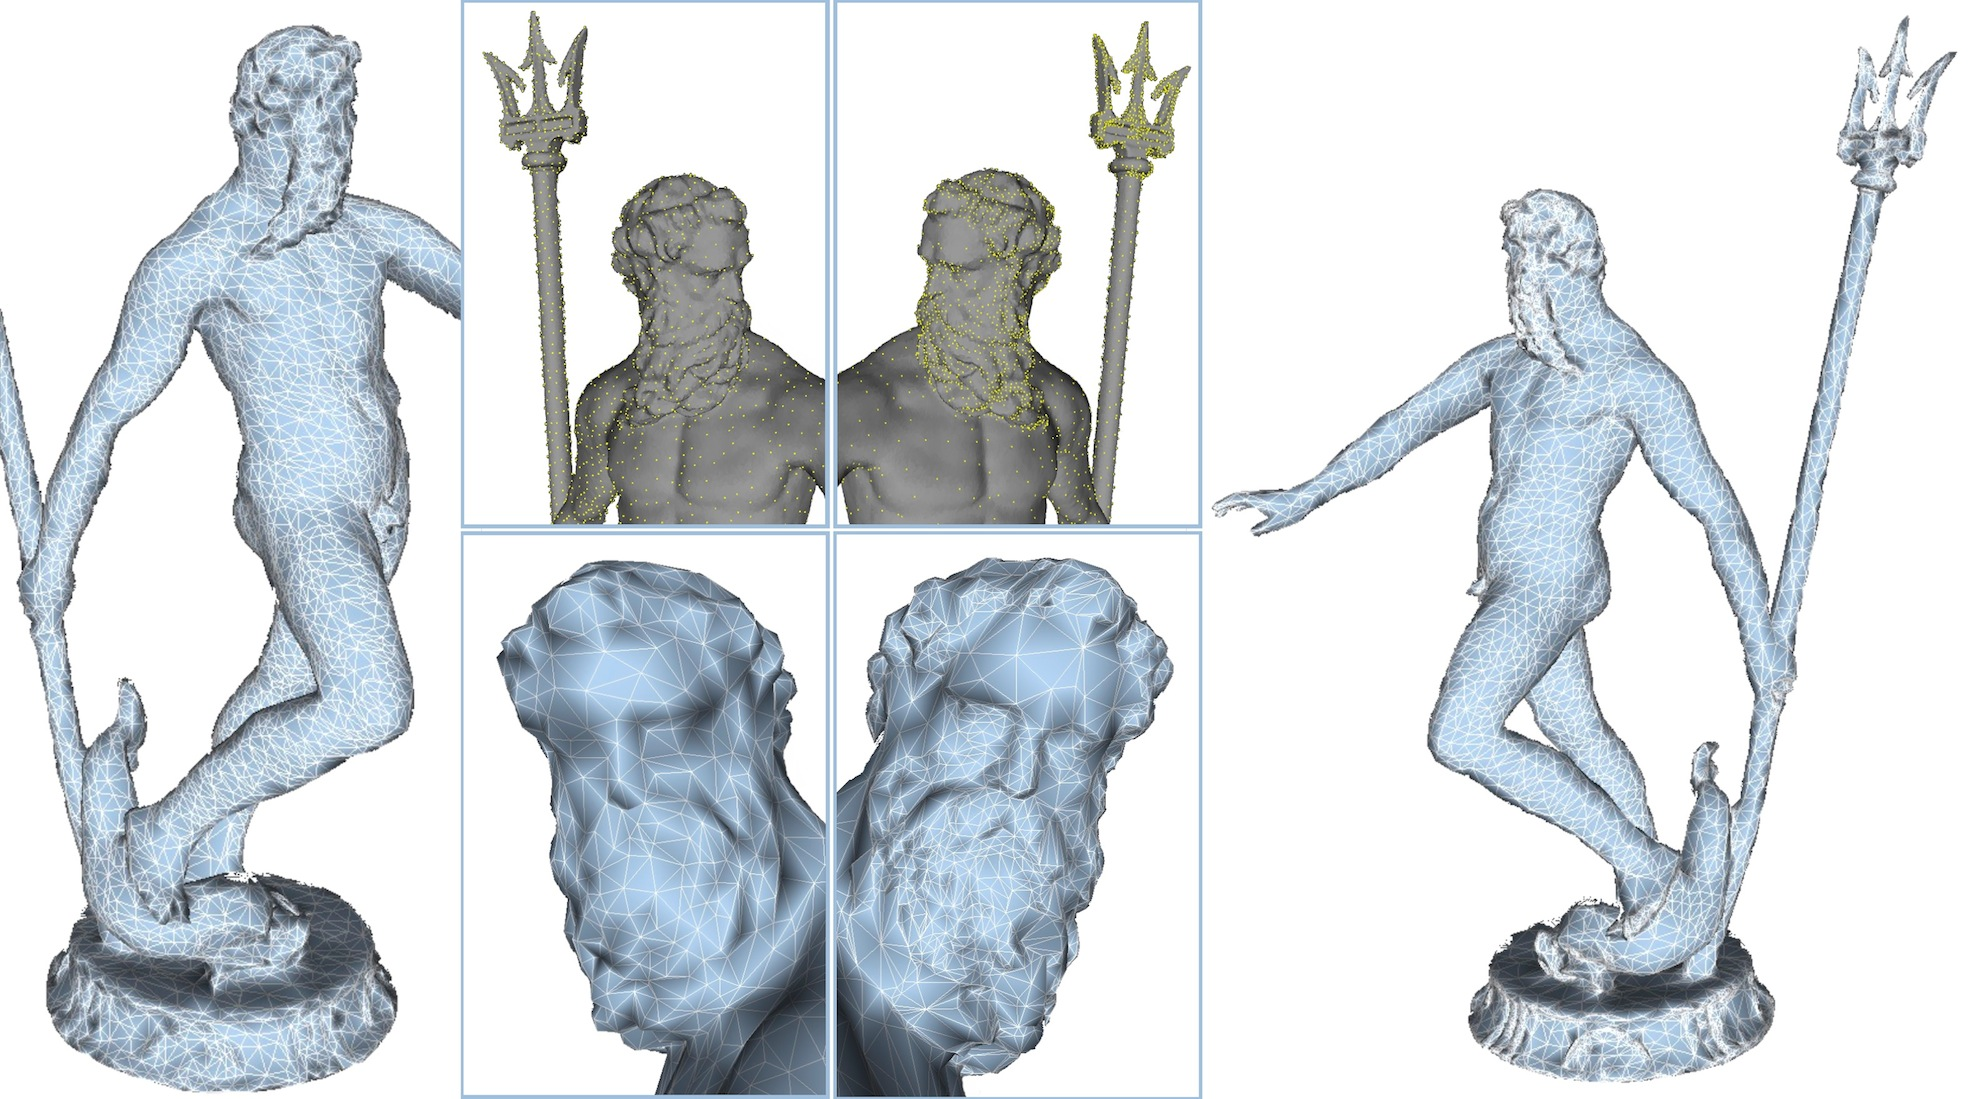
\includegraphics[width=1.0\textwidth]{adaptive_density_control.jpg}
\caption{Normal vs. adaptive density control. Whereas the sampling left shows almost uniform distribution, the adaptive version retains higher vertex counts in important regions without loosing good aspect ratios of the triangles. Note how the triangle size changes between forehead and beard.}
\label{fig:adaptive_density_control}
\end{figure}\\
We propose two simple modifications to mitigate these effects, which we call \textit{Adaptive Density Control}.
Ideally we want good triangle shapes without loosing too much geometric detail.
To solve this problem we simply vary the distance $\epsilon_{v}$ according to the weight of the vertex $\mathrm{v}$ it is associated with.
In figure \ref{fig:adaptive_density_control} are the results for the \textit{Neptune} Model.
On the left one can see the decimated mesh after isotropic or normal density control was used.
For the mesh on the right, we adapted the distance $\epsilon$ to just two values.
$\epsilon_{big}$ if the vertex weight was below the mean vertex weight: $\mathrm{x}(\mathrm{v}) < \overline{\mathrm{x}}$ and to $\epsilon_{small}$ if the vertex weight was above the mean vertex weight: $\mathrm{x}(\mathrm{v}) > \overline{\mathrm{x}}$, with $\epsilon_{small} < \epsilon_{big}$.
Note that the value $\overline{\mathrm{x}}$ gets calculated during the sampling phase and is already given at that point.

We did not specify exact values in our example, neither for $\epsilon_{big}$, nor for $\epsilon_{small}$.
The reason for this is, that instead of Euclidian distances as originally proposed, we opted for measuring the distances in terms of so called 1-rings\footnote{ This concept depends to some extend on the assumption that edge lengths will not drastically vary in local neighborhoods. We think this is a sound assumptions, for some applications like marching cubes or Delaunay generated surfaces this holds by definition. However should the user see that a given surfaces is not suitable the Euclidean distance measure with an continuous $\epsilon \in [\mathrm{d}_{min}, \mathrm{d}_{max}]$ can always be used as a fall-back alternative.}.
This means for instance, that every sampled vertex with a weight $\mathrm{x}(\mathrm{v}) > \overline{\mathrm{x}}$ only evaluates its direct neighboring vertices $\epsilon_{small} = 1$, whereas a vertex with $\mathrm{x}(\mathrm{v}) < \overline{\mathrm{x}}$ will spread out much like the cells during flood-fill.
We achieved good results for $\frac{\epsilon_{big}}{\epsilon_{small}} \geq 2$.\\
Not having to calculate Euclidian distances greatly improves the runtime, unfortunately one problem still retains that hasn't been mentioned at all, so far.
While tinkering with adaptive density control, we calculated the aspect ratios of the triangles to have quantitative benchmarks.
The aspect ratio of a triangle $\mathrm{f}$ is a dimensionless number $AR \in [1, \infty)$, that is 1 if and only if for all edges $||\mathrm{e}_{i}|| = ||\mathrm{e}_{j}||$:
\begin{equation} \label{eq:aspect_ratio}
\mathrm{AR}(\mathrm{f}) \,=\, \frac{||\mathrm{e}_{0}|| \cdot ||\mathrm{e}_{1}|| \cdot ||\mathrm{e}_{2}||}{8 \cdot (s-||\mathrm{e}_{0}||) \cdot (s-||\mathrm{e}_{1}||) \cdot (s-||\mathrm{e}_{2}||)}, ~~~~ s = \frac{||\mathrm{e}_{0}|| + ||\mathrm{e}_{1}|| + ||\mathrm{e}_{2}||}{2}
\end{equation}
%Bild
\vspace{-0.75cm}
\begin{figure}[ht]
\centering
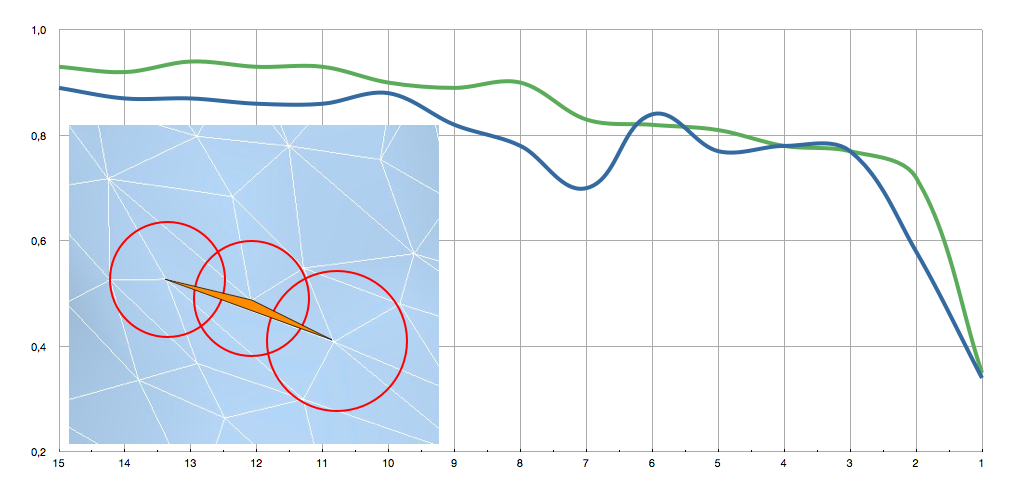
\includegraphics[width=1.0\textwidth]{bad_triangles.jpg}
\caption{Relative triangle quality, Y-axis, of normal decimation (blue) vs. density control (green), over small decimation ratios X-axis and an example of a bad triangle shape that can't be caught by density control.}
\label{fig:bad_triangles}
\end{figure}\\
After looking at the data we notices the the ratio between the mean and maximum value for all faces: $AR(\mathcal{M}) := \frac{AR_{mean}}{AR_{max}}$ did not turn out as expected.
First and most importantly, they weren't as good as hoped.
Drilling down on the issue showed that only $AR_{mean}$ improved and that $AR_{max}$ still remained high.
This is especially worrisome as for example, simulations are not resilient against single bad triangles no matter how good the rest are.
The second finding was that the ratio $AR(\mathcal{M})$ is highly volatile and can vary greatly from sample to sample.\\
In figure \ref{fig:bad_triangles} we plotted $AR(\mathcal{M})$ on the Y-axis, over the target size of the decimation, X-axis.
The blue curve is the result for decimations without any density control, and green shows the results with normal density control.
Although generally better, judging only by the diagram, density control hardly merits its expenses.
Yet, optically the results are convincing.
The phenomenon can be explained with the example from the triangulation in \ref{fig:bad_triangles}.
All three vertices of the badly shaped, orange triangle have a big surrounding that was cleared by the density control step, but still this does not guarantee good shapes, as they nevertheless can be poorly arranged.\\
In order to circumvent this problem one can run a conventional clean-up step at the very end, which also means that the runtime drastically increases.
Up to this point we do not have a viable solution that securely rids every single bad triangles from the mesh without breaking time complexity of the otherwise fast density control.


\subsection{Saving Sample Data}
\label{topstoc123}

By no means a big addition, but a helpful supplement, is the option to save the references of sampled vertices.
This is possible because the topological clustering will result in the exact same decimated mesh, as long as the order of the vertex queue $\mathrm{Q}$ is preserved and the underlying mesh does not change.\\
This enables the user to save any specific decimation at almost no memory cost.
So instead of saving the entire meshes for various discrete LODs, the user can carefully edit each version, including any manual tweaks like setting control points etc. and save only the short and efficient list of references.
Once the geometry of a mesh is loaded and only different versions are needed, this strategy can lead to huge difference in loading times, especially when dealing with big models.


\newpage
\section{Simplifying Topology}
\label{topstoc2}

\subsection{Information \& Feature Detection}
\label{topstoc21}

Our goal is to provide the user with clear and unambiguous information, so that she can easily decide whether to dismiss or keep a topological feature.
It took the entire chapter \ref{math0}, to lay down the mathematical foundations and to introduce the algorithms needed, especially the pairing of simplices \ref{algo:simplex_pairing}.
Now we want to show the results.
%Bild
\begin{figure}[ht]
\centering
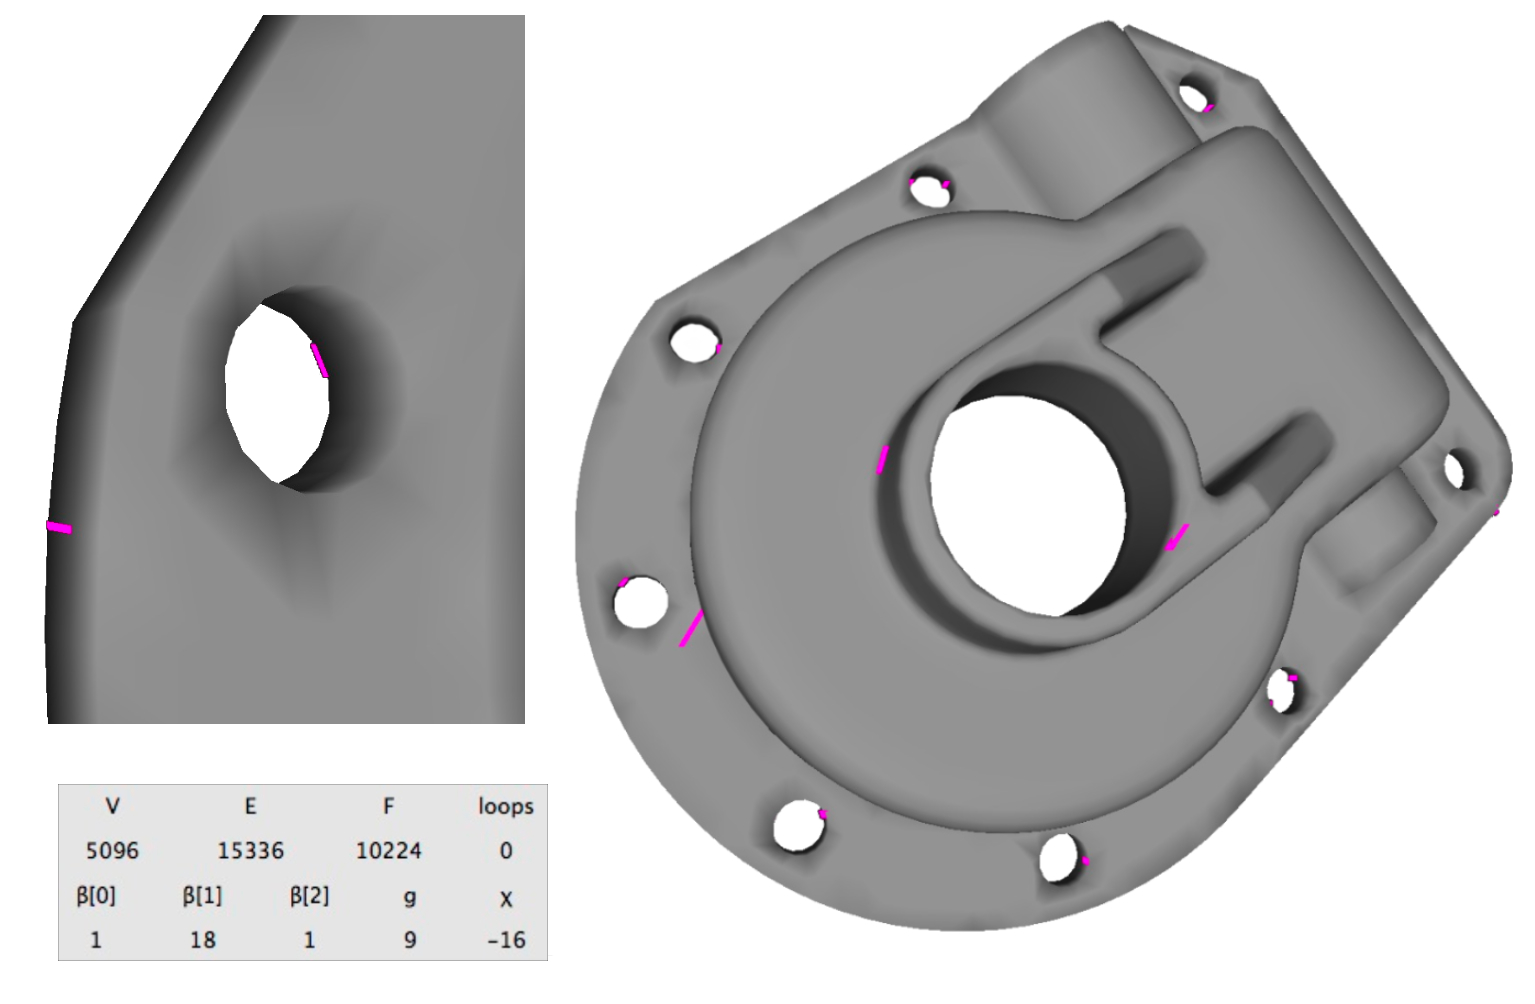
\includegraphics[width=0.85\textwidth]{casting.jpg}
\caption{The model \textit{Casting}, of genus 9 with the handle and tunnel loops inducing edges visualized.}
\label{fig:casting}
\end{figure}\\
At any time the user is presented with a control panel displaying the following topological relevant information:
%\vspace{-2ex}
\begin{itemize}
%\setlength{\itemsep}{0cm} \setlength{\parskip}{0cm}
	\item \textit{V, E, F} -- the total number of vertices, edges and faces, i.e. the number of simplices.
	\item \textit{$\beta$[0] / $\beta$[1] / $\beta$[2]} -- the Betti numbers, which are determined once all simplices of the surface mesh have been paired. As soon as the filtration finishes, the unpaired edges that define handles and tunnel can be visualized. In figure \ref{fig:casting} the mesh is of genus 9, producing 18 edges, which are colored in pink.\\The exact location of these edges depends on the filtration, however we generally observed that they mostly stick very closely to ``their'' features. The further an unpaired edge is away, the more likely it is to get paired by a positive face of low persistence as a positive face will pair with the first negative edge it encounters during the expansion of its boundary $\partial \Prefix^{+}{\sigma^{2}}$.
	\item \textit{g \& $\chi$} -- the genus respectively the Euler–Poincaré characteristic. If a boundary edge, i.e. an edge only adjacent to one face, is encountered while the mesh is loaded, the exact number of boundaries gets determined. This is necessary in order to calculate the genus: $\chi = 2-2g-boundaries$. Note that this does not apply if the mesh is already filtered, as the Betti numbers are accurate regardless whether the simplicial complex $\mathrm{K}$ is closed or not, see also equation \ref{eq:euler_poincare}.
	\item \textit{loops} -- shows either the number of open boundary loops or the sum of the handle and tunnel loops. The latter can only be detected once the mesh is closed, as their definition relies on the distinction between the inside $\mathrm{K}_{\mathbb{I}$ and outside volume $\mathrm{K}_{\mathbb{O}}$ of the mesh, see subsection \ref{math_loop_computation}.  
\end{itemize}
%Bild
\begin{figure}[ht]
\centering
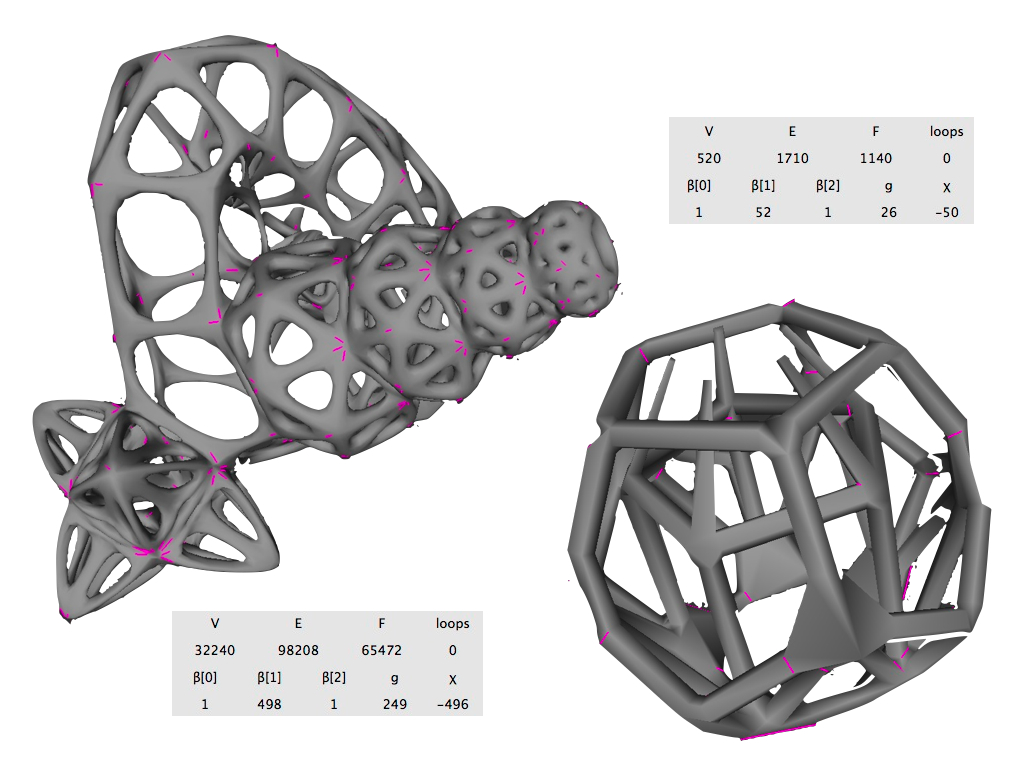
\includegraphics[width=0.95\textwidth]{high_genus.jpg}
\caption{Two ornamental models with high genera and their unpaired edges colored.}
\label{fig:high_genus}
\end{figure}\\
The decision if a particular unpaired edge gives rise to a handle or a tunnel can only be made after the simplices of the inside, respectively outside have been added to the filtration.

%Bild
\begin{figure}[ht]
\centering
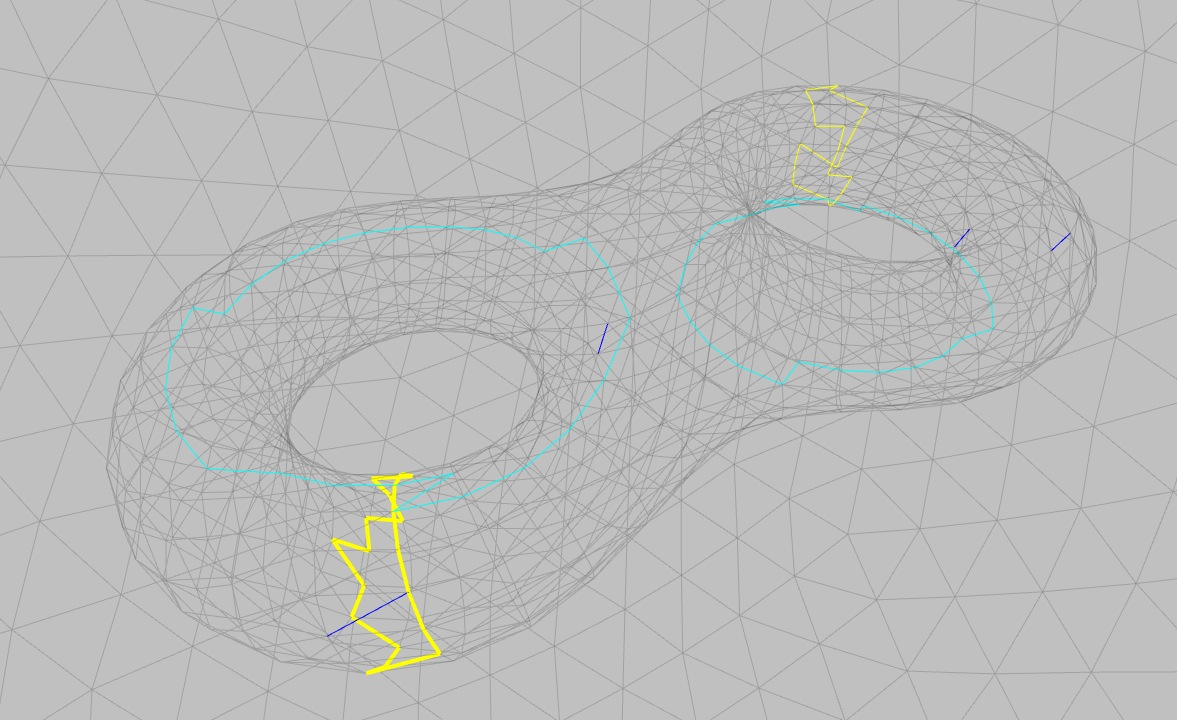
\includegraphics[width=0.775\textwidth]{found_loops1.jpg}
\caption{A tunnel (turquoise) and handle (yellow) loop of a simple double torus with its paired edges in dark blue.}
\label{fig:found_loops1}
\end{figure}\\
In figure \ref{fig:found_loops1} and \ref{fig:found_loops2} the found handle and tunnel loops are shown.
Note that the refined loops generally do not share an edge with the generating edges they are paired with.
In order to get geometrically better loops, we only safe the shortest loop, in terms of the edge count, that is entirely on the surface.
Once the loops are found, the user can cycle through them and adjust the edges individually.
Thereby adjusted handles or tunnels can be used to quickly delete unimportant parts of the mesh.
%Bild
\begin{figure}[ht]
\centering
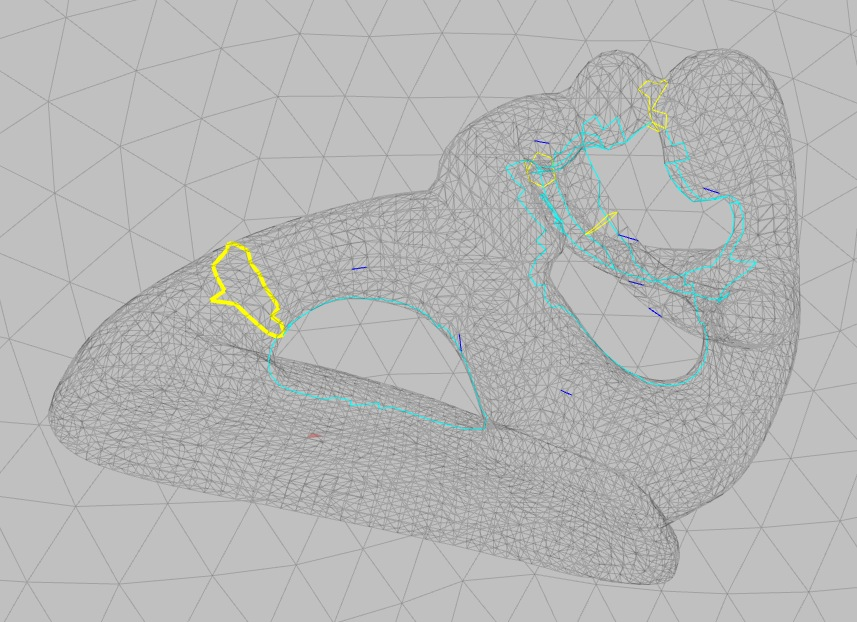
\includegraphics[width=0.75\textwidth]{found_loops2.jpg}
\caption{Model \textit{Mother} with its tunnel (turquoise) and handle (yellow) loops.}
\label{fig:found_loops2}
\end{figure}\\
Note that the complexity of the pairing algorithm does not depend on the genus, only on the total number of simplices $|\sigma^{n}|$ with $n>0$, that constitute $\mathrm{K}$.
It is further noteworthy that the time needed to pair all simplices of a dimension $n>m$ gets exponentially bigger as not only the size of the boundary $\partial_{n} > \partial_{m}$ increase, but also with it the number of chain elements that get introduced during every step of the expansion.

Just pairing the simplices of the surface, typically takes only a matter of seconds for meshes with less than 100,000 faces and is negligible for meshes below 25,000 faces.
Unfortunately, the pairing of faces from the inside and the outside scales far worse than we initially expected.
It exceeds the minute mark even for meshes with less than 50,000 faces.
This is due to the tetrahedralization, as the number of total simplices increases with a factor of about five.
During our tests, the pairing of vertices and edges normally took less than 15\% of the total time.
This is concerning, mainly because we stopped pairing faces from the inside and the outside once the handle and tunnel loops where found, i.e. only paring less than half of the entire amount.

This compels us to acknowledge that finding topological accurate loops via filtration, is not a good fit with ``TopStoc''.
It could be argued, that this step should be skipped, pairing only the generating edges.
This sounds unintuitive, but it is a valid point, especially since the unpaired edges are enough to indicate topological features and most importantly guaranteed to be mathematical correct.
The user has enough information to decide if she wants to alter the topology or not and that is what we set out to achieve.
So one possible direction to pursuit is to filter the surface mesh, thus ensuring that all important features get represented, but then switching to a cheaper heuristic to find loops.

\subsection{Mesh Editing}
\label{topstoc22}

Independent of feature detection, the user always has the option to manually select any face of the mesh and delete it.
Besides the deletion tool, the users second instrument to change topology is the retriangulation of a boundary loop.\\
In figure \ref{fig:cut_and_mend} this is shown exemplarily for a double torus that gets dissected by hand in two places.
The deletion on the left kills a handle loop and the deletion on the right kills a tunnel loop.
After the cuts, the mesh gets filtered again to update the Betti numbers -- note that $\chi$ remains -2, this is not an error, it is correct for the reason that we introduced 4 new boundaries.
To indicate the boundaries, the vertices on them are colored red.
As long as the mesh has open boundaries, the user can cycle through them via buttons and retriangulate them\footnote{ Retriangulating holes in surface meshes, is by no means a trivial task and many papers have been published, devoted to answering this question \citep[cf.][]{Zhao2007}. Yet, we assume that any hole filling happens at places of minor importance, typically to mend the mesh after an unimportant feature has been deleted. Additionally we don't care for the quality as long as it produces a water-tight sealing. Consequently we do not deploy a sophisticated scheme but instead project the boundary onto a plane and use a 2D triangulation algorithm to solve the problem.}.
The selected boundary is highlighted in yellow.\\
%Bild
\begin{figure}[ht]
\centering
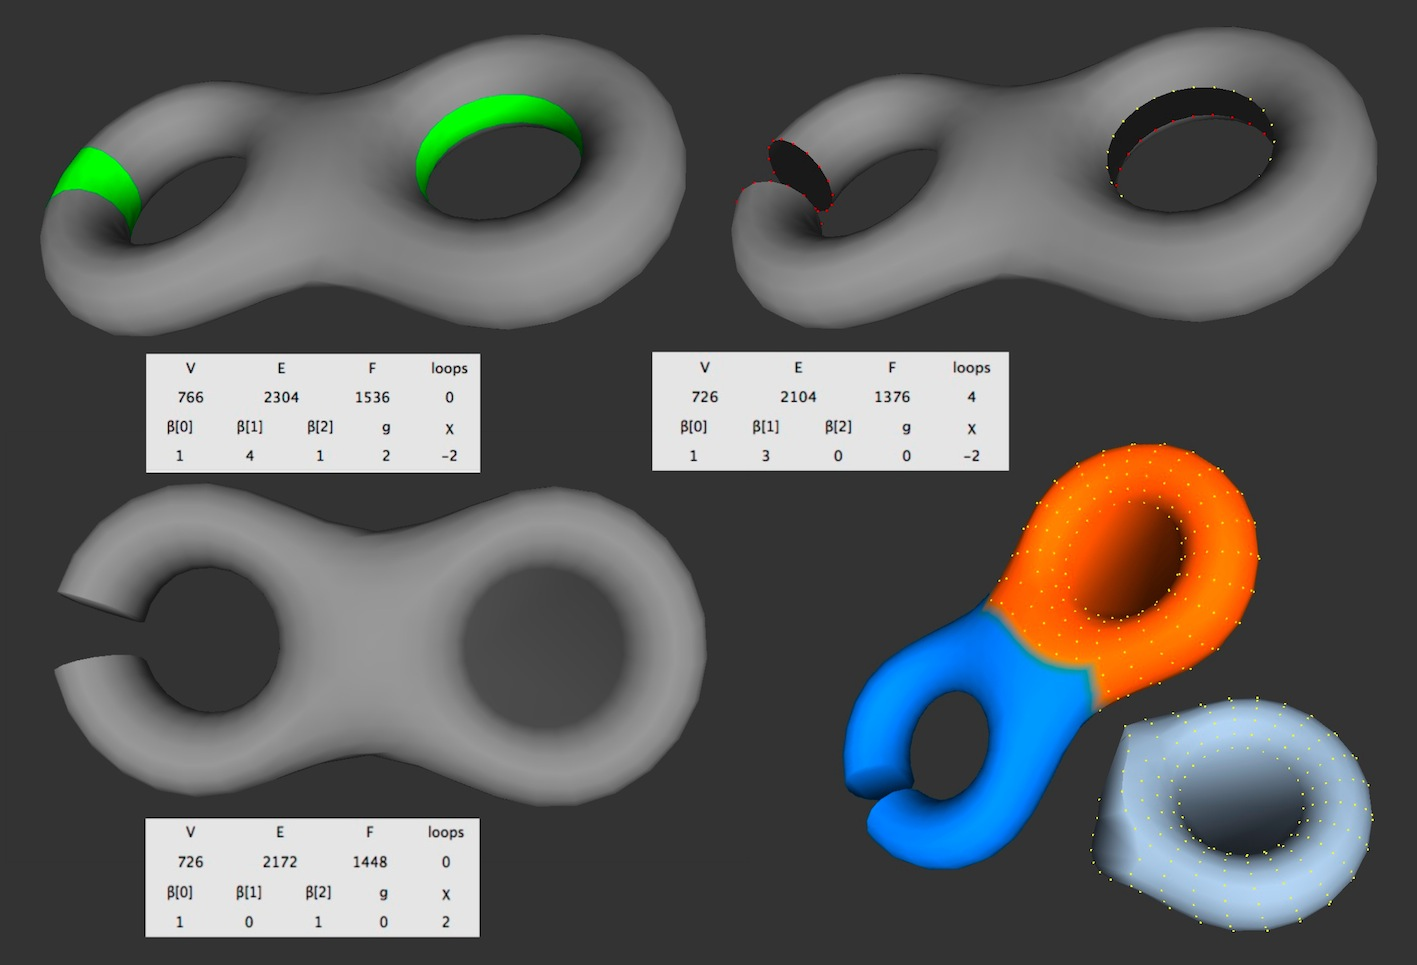
\includegraphics[width=1.0\textwidth]{cut_and_mend.jpg}
\caption{Topological operatons on a double torus.}
\label{fig:cut_and_mend}
\end{figure}\\
After the four boundaries are retriangulated the mesh is topologically equivalent to a sphere as indicated by the invariants.
To further prove the successful transformation we set the sampling probability for half of the mesh to zero and to one for the other half -- the blue region and orange regions.
On the lower right of figure \ref{fig:cut_and_mend} is the outcome, a decimated mesh with genus null.

\newpage
\subsection{Limitations}
\label{topstoc23}

There are two limitations to consider when working with the current implementation.
The first is, that it was designed to work with one single connected component at a time.
If a mesh gets partitioned into two individuals parts, the program has no way to display the topological invariants individually.
Reckoning the change, however is trivial as $\beta^{0}>1$.
Interestingly enough though, the pairing algorithm does still work and the values for the Betti numbers represent the summed up results, see figure \ref{fig:g3_cut}.
Note that although the Betti numbers are correct, the displayed genus for the second mesh is wrong.
At this point, reconnecting parts that were split before, is not supported. 
%Bild
\begin{figure}[ht]
\centering
\includegraphics[width=0.75\textwidth]{g3_cut.jpg}
\caption{A mesh $g=3$ that gets severed into two parts, with $g_{1}=0$ and $g_{2}=1$ .}
\label{fig:g3_cut}
\end{figure}\\
The second restrictions concerns not orientable surfaces.
This is more of a barrier, as the pairing algorithm completely fails and even displays boundary vertices for the completely closed mesh.
Even our viewport fails in the face of this challenge, when asked to render triangles, as seen on the right sight of figure \ref{fig:klein_bottle}.
For that matter, the TopStoc algorithm can't be convinced to work with this type of meshes either.
%Bild
\begin{figure}[ht]
\centering
\includegraphics[width=0.70\textwidth]{klein_bottle.jpg}
\caption{The Klein bottle withstands filtration and decimation by our methods.}
\label{fig:klein_bottle}
\end{figure}


\section{Drawing on Meshes}
\label{topstoc3}

We now turn to the very heart and epitome of user-guidance, that is the explicit control over the decimation process\footnote{ User-guidance, somewhat unexpectedly, hasn't been of much interest in the last years as far as research papers are concerned. The work that still gets published, mostly reprises unimaginative adaptations of known decimation schemes to work with user input \citep[cf.][]{Ho2006}. This is astounding as the very first work already set a different trajectory by discussing among other things response times, i.e. work-flows \citep[cf.][]{Cignoni1998a}.}.\\
Although a major aspect of our work and an extremely powerful tool to selectively increase the fidelity of a mesh, the concept and implementation with ``TopStoc'' is strikingly unproblematic.
This is due to the fact that other decimation techniques are based on intangible error-bounds or priority queues, whereas our approaches rests on stochastics which are intuitively clear.
This way, instead of just attributing certain regions of a mesh with immunity to decimation, or fiddling with abstract rules and weights, the user can just literally 'sketch probabilities' onto the base mesh.
%Bild
\begin{figure}[ht]
\centering
\includegraphics[width=1.0\textwidth]{planes.jpg}
\caption{Vertices on the wings of the plane are either kept or dismissed entirely (bright orange or dark blue). The body gradually gains geometric detail from top to back. On the plane in the middle, the then sampled vertices are shown and on the right is the final mesh alone.}
\label{fig:planes}
\end{figure}
In the example of figure \ref{fig:planes} the various parts of the plane model were painted with different probability levels.
Orange depicts values of relatively higher probability and blue levels of lower probability in respect to grey, which always conforms to the global target size that was set by the user.
Having the same effect as if each part of the model was processed individually with its own decimation ratio.\\  
This means that, for example, if the user adjusts the slider to a 0.5 the orange parts cover decimation ratios between $[0.5,1.0]$ and the likewise the blue areas cover $[0.5,0.0]$.
This seems to be problematic if the overall decimation ratio closes in on either boundary $1.0$ or $0.0$ and the colors encode less and less equal parts of the entire decimation range.
However, the design was a deliberately chosen, since this way one has a unambiguous and obvious feedback which parts were tweaked by the user to use less geometric detail and which parts needed to be boosted.
Furthermore the application offers the user a finely partitioning of each side, orange and blue, so that even in the most extreme cases the adjustability is ensured. 
%Bild
\begin{figure}[ht]
\centering
\includegraphics[width=0.80\textwidth]{controlpoints.jpg}
\caption{Besides the fuzzy painting of entire regions, the user has also the option to select a set of single elements and set their probability individualy.}
\label{fig:controlpoints}
\end{figure}\\
Note that the incorporation user-guidance does not impact the speed of the algorithm, as it only adds additional information for each vertex but does not require additional processing.
It is important to mention though, that once a region is augmented with user-set probabilities, the resulting mesh size after the decimation will deviate from the target size.
User-input always trumps automatic adjustment and enforcing the precise target size would lead to higher runtimes. 
%Bild
\begin{figure}[ht]
\centering
\includegraphics[width=1.00\textwidth]{sketchy_regions.jpg}
\caption{Another example of how user-assistance can lead to better results. Left is the unaltered result, right the improved version, note that both versions were sampled to the same vertex count $\pm$1\%.}
\label{fig:sketchy_regions}
\end{figure}

\newpage
\section{Back-face Subsampling \& Silhouette Preservation}
\label{topstoc41}

View-dependent decimation reckons that most of the time, only a fraction of the geometric detail is visible to us and that a good decimation scheme should exploit this.  
To leverage this fact, at least the direction of the camera is needed, achieving its full potential if a complete frustum is defined, as model parts outside the frustum can be dismissed entirely.
Together with the view-direction comes the concept of silhouettes, which are of pivotal importance for the perception of detail and geometric fidelity.
As early as 1996 appeared papers dealing with simplification methods that paid special attention to these details \citep[cf.][in which, not only view-dependencies but also decimation adapting to lighting conditions, gets discussed]{Xia1996}.
%Bild
\begin{figure}[ht]
\centering
\includegraphics[width=0.90\textwidth]{armadillo_pov.jpg}
\caption{The \textit{Armadillo} model, showing the sampled vertices on the front and the back, with the resulting mesh in the middle.}
\label{fig:armadillo_pov}
\end{figure}\\
As in the case with user set decimation ratios, once again the ``TopStoc'' algorithm lends itself almost effortless to an adaption for silhouette preservation and back-face culling.
Remember that the weight for vertices, as introduced in equation \ref{eq:vertex_weight} already uses normals.
Therefore this technique more or less inevitably suggests itself to be adapted, as soon as a view-vector $\mathrm{v}_{cam}$ is defined: $\mathrm{x}_{view}(\mathrm{v}) \,=\, (\textbf{n}^{T}_{v}\textbf{v}_{cam})/2$\\
Of course it is possible to introduce $\mathrm{v}_{cam}$ directly to equation \ref{eq:vertex_weight}, not adding it as an extra value to each vertex like we propose.
This undeniably would lessen the computational impact, offering back-face subsampling and silhouette preservation at no additional cost.
However this also means that all given weights have to be recalculated every time $\mathrm{v}_{cam}$ changes, even if only a normal decimation is desired.\\
%Bild
\begin{floatingfigure}[r]{0.31\textwidth}
%\begin{figure}[ht]
\center
\includegraphics[width=0.29\textwidth]{armadillo_pov_hausdorff.jpg}
\caption{Errors per Triangle.}
\label{fig:armadillo_pov_hausdorff}
\end{floatingfigure}
%\end{figure}
In figure \ref{fig:armadillo_pov} the effect for a considerable lower sample rate on the back-face is shown.
Making use of a point of view aware decimation immediately drops the geometric complexity nearly by half, for the same accuracy of visible parts\footnote{ Depending on the geometry and the extend to which the object is concave -- with most organic models being very suitable, but hard surface models posing a bigger challenge.}.
To give a further impression of the results, we visualized the errors per triangle for the decimated mesh from figure \ref{fig:armadillo_pov}, see figure \ref{fig:armadillo_pov_hausdorff}.\\
Another interesting result is that since the ``TopStoc'' algorithm preserves the topology of an object we can cull faces on the backside of models altogether, still ending with a water-tight mesh at the end.
However, it is desirable to preserve vertices that lie on the silhouette to avoid artifacts that could otherwise result from the culling.\\
Silhouette preservation in itself is not an independent step as exactly the same normal calculation takes place.
The difference is that a values close to zero are dealt with more attention. 
Also for the practical applications it is necessary to define an interval for a graceful diminish, see the model on the right in figure \ref{fig:silhouette}.
This amends the problem that the area at the silhouette is not necessarily friendly towards such a treatment, unless the body is perfectly concave, obviously. 
%Bild
\begin{figure}[ht]
\centering
\includegraphics[width=1.0\textwidth]{silhouette.jpg}
\caption{Back-face culling and silhouette preservation are demonstrated on a sphere. On the left is the error visualization, next to it the GUI panel for the feature, in the middle is the decimated mesh with the sampled vertices colored and on right, the same model with a bigger aperture of the silhouette.}
\label{fig:silhouette}
\end{figure}
%Bild
\begin{figure}[ht]
\center
\includegraphics[width=0.29\textwidth]{pov_limitation.jpg}
\caption{Oversampling on ill-formed silhouette areas.}
\label{fig:pov_limitation}
\end{figure}\\
Unfortunately there are bad cases in which the preservation of the silhouettes not necessary fails, but yields really unwanted results.
Figure \ref{fig:pov_limitation} shows such a situation in which the silhouette coincides with a planar region, preserving way too many vertices.
This problem can be solved though by user intervention.
Painting with value -1, i.e. the dark blue, overrides any sampling decisions by the the algorithm.
All in all are the tools connected with the point of view a very helpful addition at negligible costs.


\section{Textures}
\label{topstoc42}

A key component in making any decimation method feasible for the actual adaptation in other field besides academia is the support for texture handling.
The role that textures play in fields like \textit{Computer Games} or the \textit{VFX} industry can not be overstated.
Actually the success of wrapping geometry with 2D images for various scenarios like bump-mapping, displacement information, dirt layers, etc. has to some extend fallen victim to its own success, but although more sophisticated solutions are available, like \texttt{Ptex}\footnote{ The idea behind this concept proposed by \textit{Burley} and \textit{Lacewell}, is to assigns an entirely separate texture per face, skipping the texture unwrap entirely.  The technique uses adjacency data to filter across faces, removing otherwise visible seams.}, conventional textures will be around for years to come \citep[cf.][\texttt{Ptex} opposed to MeshColors is a fully-fledged concept that has been already successfully used]{Burley2008}.\\
Because of this, it was important for us to include texture handling and support.
The problem when decimating meshes that normally hold textures is that highly visible artifacts appear if the borders of the so called UV patches are not respected.

%Bild
\begin{figure}[htb]
\center
\includegraphics[width=0.66\textwidth]{uv_mapping.jpg}
\caption{Model with UV layout, image courtesy of \href{http://blogs.gscept.com/2008/sg2/index.php/page/2/index.html}{World Of RaftCraft}.}
\label{fig:uv_mapping}
\end{figure}\\
Figure \ref{fig:uv_mapping} shows a model together with its UV layout.
Note that color between the patches is normally black, so what one will typically see if a UV border vertex gets deleted is that the model has strange dark patches on its surface.\\
The easiest remedy to tackle this problem is to check which vertices have multiple texture coordinates as this defines the vertices on the border of UV patches.
Any of these can subsequently set to ``untouchable'' to ensure that no border gets lost.
This is what we implemented and is shown in figure \ref{fig:dec_texture}.
%Bild
\begin{figure}[htb]
\center
\includegraphics[width=1.0\textwidth]{dec_texture.jpg}
\caption{Modell ``Mini Cooper'' courtesy of \href{http://www.oyonale.com}{Oyonale}.}
\label{fig:dec_texture}
\end{figure}\\
The Mini on the left is the base mesh, on the right is the decimated version, note the high vertex density around the doors where a UV border resides.
At more sophisticated approach is to flood-fill the vertices of each patch to know, not only if a vertex lies on the boundary but also which specific patch it belong to.
This in turn makes it possible to redraw the texture and avoid artifacts altogether, well besides artifacts of distortion which would require even more subtle handling\footnote{ At this moment our reference implementation supports the preservation of vertices that have multiple texture coordinates, but we haven't pursuit any further so far.}. 


\section{Bounding Boxes \& Materials}
\label{topstoc43}

Last but not least is the support for bounding boxes and materials definitions.
These two items are not orthogonal to the rest of the tool set, so to say.
They \textit{only} facilitate the work for the user when dealing with models, but the effects could also be achieved if only using the previously described methods.

Support for bounding boxes entails the option to specify a series of cuboids.
Vertices that happen to be in any of such a volume get assigned one common weight.
This for instance is helpful to define frustums that cull an object.\\
Considering materials has a similar effect only that the familiarities of vertices are not defined by proximity but instead by the material definition given in the source file.
Almost all standards for geometry representation include such material definition and are normally used for rendering and shader binding.


\newpage
\section{Meassurements}
\label{topstoc5}

The evaluation of the results falls into two domains, on the one hand there is the individual perception of the user and on the other hand there are precise mathematical error bounds.
The user will typically make the final decision whether a certain asset holds up to his or her standards judging by the optical impression.
Yet, it is is also important to be able to get unequivocal data to rely on, for instance if simulations are involved.\\
We want to cater both scenarios as they are equally important.
Consequently we implemented one distinct tool for each one of them, not only to give feedback, but also to help guiding an iterative workflow.
% Bild
\vspace{0.2cm}
\begin{figure}[ht]
\begin{minipage}[b]{0.425\linewidth} \centering
\includegraphics[height=3.0cm]{mesh_information.jpg}
\caption{Basic information, vertex count of the meshes.}
\label{fig:mesh_information}
\end{minipage}
\hspace{1.0cm}
\begin{minipage}[b]{0.5\linewidth}
\centering
\includegraphics[height=3.0cm]{metrics_tab.jpg}
\caption{Metrics tab with the 'Hausdorff' and 'Multiview' section.}
\label{fig:metrics_tab}
\end{minipage}
\end{figure}\\
The basic information of the amount of vertices in the base mesh and the decimated mesh, is of course always shown.
Additionally, the tab labeled 'Metrics' offers the calculation and visualization of the Hausdorff distance, as well as the 'Multiview' tool which spawns new instances of the current decimation settings with limited variation, which will be both described in sections \ref{topstoc51} and \ref{topstoc52}.\\
Another useful utensil in assessing the decimation quality, is the turntable button.
When pressed, the mesh is placed in the center of the screen and the camera then gyrates two times around the model in an upwards spiral to show all the mesh from all direction.
%Bild
\begin{figure}[ht]
\centering
\includegraphics[width=0.85\textwidth]{turntable_dragon.jpg}
\caption{Turntable of the decimated dragon mesh, with Hausdorff distance visualized.}
\label{fig:turntable_dragon}
\end{figure}

\subsection{Hausdorff Distance}
\label{topstoc51}

In the case of 1D-signals and images, many distortion measurements have been studied.
They range from simple analytic methods such as the mean square error to very elaborate techniques based on the characteristics of human perception \citep[cf.][]{Winkler2001}.
Despite the constantly growing usage of 3D models, the distortion measurements for such data seem to be less thorough.
Still the predominant approach to compare two meshes is the \textit{Hausdorff distance}\footnote{ First introduced in the book \textit{Grundzüge der Mengenlehre}, published in 1914 and named after the German mathematician \textit{Felix Hausdorff} (1868 – 1942), one of the founders of modern topology. Technically the Hausdorff distance it is not a real distance function since it lacks symmetry. It is better to think of it in terms of set containment, for more information and examples see Appendix \ref{appendix5}.}, defined as:
\begin{equation} \label{eq:hausdorff}
\hspace*{0.5cm} d_{\mathrm H}(\mathcal{M},\mathcal{M}') = \sup_{p \in \mathcal{M}} \inf_{p' \in \mathcal{M}'} d(p, p')
\end{equation}
respectively the symmetric version:
\begin{equation}
d_{\mathrm H_{sym}}(\mathcal{M},\mathcal{M}') = \max \{\sup_{p \in \mathcal{M}} \inf_{p' \in \mathcal{M}'} d(p, p')~, \sup_{p' \in \mathcal{M}'} \inf_{p \in \mathcal{M}} d(p', p)\}
\end{equation}
Where the distance $d(p, p')$ between two points $p$ and $p'$ on the surfaces of the mesh $\mathcal{M}$ and it's simplified version $\mathcal{M}'$ is defined as: $d(p, p') = || p-p' ||$ with $||.||$ denoting the usual Euclidean norm.
We will refer to $d_{\mathrm H}(\mathcal{M},\mathcal{M}')$ as the forward distance, and to $d_{\mathrm H}(\mathcal{M}',\mathcal{M})$ as the backward distance.\\
The distance between any point $p$ belonging to $\mathcal{M}$ and $\mathcal{M}'$ can be computed analytically, since it can be reduced to the minimum of the distances between p and all the triangles $\mathcal{F}_{\mathcal{M}'}$.
It is worth noting that $p$ might not be a vertex of the list $\mathcal{V}_{\mathcal{M}}$ but any point on the surface.
Hence, although straightforward, the algorithm becomes too complex if implemented naively\footnote{ In fact, for each sample point $p$ it would be necessary to calculate the distance to all triangles $\mathcal{F}_{\mathcal{M}'}$ in order to find the minimum.
This leads to a complexity $\mathcal{O}(|p| \cdot |\mathcal{F}_{\mathcal{M}'}|)$, where $|p|$ is the number of sample points taken on $\mathcal{M}$ and $|\mathcal{F}_{\mathcal{M}'}|$ is the number of triangles.}.
To achieve reasonable running times we followed the implementation strategy described in the paper \textit{``Mesh: Measuring errors between surfaces using the hausdorff distance''}, where a cell partitioning strategy is used to greatly reduces the number of point-triangle distance evaluations.
Each triangles is sampled via a regular grid according to a length criterion, thus avoiding uniform sampling \citep[for more details see][especially chapter 3]{Aspert2002}.

By pressing the 'Hausdorff' button the backward distance is calculated and the numerical values for mean and maximum distances are shown.
Since the algorithm maintains a 1-1 correspondence between the sampled points and the base mesh, calculating the forward distance would yield little information and is omitted to save time.
%Bild
\begin{floatingfigure}[r]{0.31\textwidth}
\center
\includegraphics[width=0.29\textwidth]{hausdorff_colors.jpg}
\caption{Visualization Hausdorff.}
\label{fig:hausdorff_colors}
\end{floatingfigure}
More important for the practicality though, is that the normalized error values can be used to colorize the decimated mesh.
Thereby giving the user a clear representation of errors in the form of darkened triangles.
In image \ref{fig:hausdorff_colors} the upper sphere shows the gradually loosening of fidelity on the base mesh in colors.
Starting at the orange section on the upper left, where almost all vertices are sampled, the sampling rate steadily diminishes until it is below 1\% in the dark blue area.
The second lower sphere shows the decimated mesh with the visualization of the Hausdorff distance at each triangle.

The user can then switch between the the two visualization modes and selectively set control points on the base mesh to improve the quality in certain regions that would be otherwise undersampled.
In figure \ref{fig:hausdorff_control_points} the mesh is sampled at the same decimation rate of about 9,000 vertices two times, only deviating at less than 1\% of the total number.
However, for the second sampling, a series of control points were inserted in the areas of the cheek, forehead and the throat.
Giving a better overall result for the mean error of the Hausdorff distance.
%Bild
\begin{figure}[ht]
\centering
\includegraphics[width=0.55\textwidth]{hausdorff_control_points.jpg}
\caption{Two versions of a bust, with the same vertex count, but on the left hand side without control points to avoid undersampling.}
\label{fig:hausdorff_control_points}
\end{figure}

\subsection{Multiview}
\label{topstoc52}

With the Hausdorff distance at his disposal, the user is equipped to make very precise augmentations to a mesh and evaluate them quickly.
This complements the principle gauge tool for any decimation, that is the target size.
Even so, we think, that another tool has its place in this ensemble.\\
Multiview rests on the idea that it can be very beneficiary to get quick iterations with some variation of one and the same result.
The sampling algorithm is inherently stochastic and therefore will produce different versions albeit respecting constrains like user-set control points and the target size of the mesh.
We use this fact to offer the user the chance to create multiple instances of his decimation with just one single click.\\
%Bild
\begin{figure}[ht]
\centering
\includegraphics[width=1.0\textwidth]{multiview.jpg}
\caption{Four versions of a mesh with 3\% variance of the number of vertices.}
\label{fig:multiview}
\end{figure}\\
There are only two input variables that have to be defined, that is the maximal allowed variation in terms of \% mesh size and the number of instances that should be generated.
Using Multiview is possible because sampling and remeshing are comparatively inexpensive.
However with very large models it is advisable to restrict the newly instantiated windows to a small number.\\
Once the different models are created the user immediately sees whether it makes sense to persuit even lower decimation rates or if he already is at a threshold of accuracy he does not want to cross.
Besides giving fast visual feedback, Multiview can also be used to rapidly save multiple LOD versions if the variance is set to high percentages.

\chapter{Conclusion}
\label{conclusion0}

\begin{flushright}
\textit{``\,... in life we ultimately pursue, not conclusions, but beginnings.''}\\
-- Sam Tanenhaus \citep[American historian, in:][]{Tanenhaus1986}
\end{flushright}

%\newpage
%\vspace*{1ex}
\section{Summary}
\label{conclusion1}

In the beginning we tried to clarifying why mesh decimation is and will continue to be an important issue, as model complexity is still on the rise.
We also mentioned the importance of work-flows and time regimes that often get overlooked but fundamentally determine how a tool is seen and used.

In the second chapter, we looked at the spectrum of available concepts to simplify geometry and ways to categorize them.
This lead to a taxonomie and a checklist in which we formulated our goals.
But before we could evaluate our results, we gave an introduction to the mathematical concepts that were necessary in order to master the topological challenges.
In contrast to most of the previous work, we decided to implement a mathematical more demanding approach that relies on persistent homology but guarantees to find all topological relevant features.\\
Although this gave us very good results, it turned out that calculating the defining loops, breaks the otherwise fast decimation pipeline.
Fortunately we are still equipped with all the necessary information, as single edges take on the role of indicating topology.
Nevertheless we think that the processes can still be improved and might turn out to be viable in terms of time complexity after all, see \ref{conclusion22}.

Besides the topology we also tried to make sensible additions to the base algorithms and extend the scope of application to take full advantage of user input.
Additionally we addressed some practical issues like how to best measurement decimation, support textures, or in cooperate point of view decimation -- which fit really nice to the decimation pipeline.

As a result, ``TopStoc'' in its current iteration not only offers fast and robust automatic decimation, but can take full advantage of user-guidance.
In the interplay between the program and the user, the user is not restricted to some selected features for improving the results but instead really has full control over the entire decimation process, as well as the topology!

%\newpage
%\vspace*{1ex}
\section{Future work}
\label{conclusion2}

One can think of numerous little improvements and extras, that would help the workflow.
Among them are additional tools for topology control or mesh manipulation.
The optimization and the parallelization of the algorithms, also seem to pose legitimate research question.\\
Having said that, we want to focus the discussion on two entirely different issues.
The first question in section \ref{conclusion21} is motivated by the standards used in the industries, which are currently dealing with biggest assets and therefore would be the most likely candidates to adopt any of the presented results.
In short, the problem is, that for various reasons quad meshes are the quasi norm for many applications.
Yet it is not clear how the remeshing part could be adopted in a smart manner to provide for quad meshes.\\
The second question in section \ref{conclusion22}, reviews ideas of how the calculation of the Betti numbers could be sped up.
The main idea being, that a locally restricted algorithm would not only decrease running times but also improve the geometrical significance of our results.

\subsection{Adaption for Quad-Meshes}
\label{conclusion21}

The problem of generating high quality quad meshes from triangle meshes or point cloud data has been fairly well researched.
Including several surveys on the topic \citep[cf. ][]{Alliez2005, Hormann2007}.
The reason for the interest in quad meshes is, that it converts raw geometric data into a higher representation that is suitable for sophisticated operations like texturing, subdivision and compression.\\
Constructing good meshes is still hard task though, not only are there a series of quality criteria like 'edge-flow', 'individual element quality', etc. but their optimization often requires the consideration of global dependencies.
Therefore to implement a naïve quad meshing scheme after the stochastic vertex selection phase should be rather straight forward \citep[cf.][]{Li2009}, but doing it with good results and some flexibility in terms of what criteria to optimize isn't \citep[][]{Bommes2009}.
More importantly, whatever strategy gets deployed, it should take full advantage of the levers that are already in place.
What we mean by that is, that there are parts like loop computation that could be exploited to guide the meshing scheme.
%Bild
\begin{figure}[ht]
\centering
\includegraphics[width=1.0\textwidth]{dual_loop_meshing.jpg}
\caption{BLA \citep[cf.][]{Campen2012}.}
\label{fig:dual_loop_meshing}
\end{figure}\\
Just now, \textit{Campen et al.} presented a novel approach, called ``Dual Loops Meshing'', to get high quality, coarse, all-quadrilateral patch layouts on manifold surfaces \citep[][]{Campen2012}.
Their method uses a field of principal curvature directions, to get a collection of transversally crossing loops on the surface.
These loops partition the surface into polygonal regions whose valences are connected to their total curvature, see figure \ref{fig:dual_loop_meshing}.
And although we haven't analyzed the actual familiarities between their concept and the techniques we use, it is clear that they are related and could generate synergies.


\subsection{Fast $\beta^{1}$ Calculation via Decimation \& Segmentation}
\label{conclusion22}

Throughout the thesis we calculated all the Betti numbers for entire meshes, yet this seems to be unnecessary wasteful since large parts of the model are just not important, i.e. bearing $\beta^{1} = 0$.
Especially as the used pairing algorithm, described in \ref{algo:simplex_pairing}, does not scale very well.
The reason for that is, that the expansion of chain complexes in the \texttt{while loop} \,gets considerably more computational expensive as the size of the simplicial complex \mathrm{K} increases and with it, its chains.
We think that there could be ways to exclude the pricy calculation of $\beta^{2}$ in favor of smart heuristics, thereby gaining huge speed-ups.
Even if that should turn out, not to work, two further ideas could yield valuable improvements.\\
First it could be tried to quickly segment the mesh into topological meaningful parts.
Ideally one would try to dismiss as much segments, with genus null, as possible.
Thus, leaving only a smaller subset for the more involved computations.
This should be feasible since checking the topological importance is very cheap and calculated via the linear sum over the simplices.
Breaking up the problem into smaller parts provides further advantages for later stages of the process.
In case of searching for handle and tunnel loops, this would also make the tetrahedralization faster, and place the generating edges closer to the features they represent.
On top of all of that, could the smart segmentation of a mesh lead to a parallelization of the algorithm that might even lends itself to a GPU implementation -- altering the running times of these computations rather orders of magnitude than just some percentages.
%Bild
\begin{figure}[ht]
\centering
\includegraphics[width=0.60\textwidth]{betti_segmentation.jpg}
\caption{Example of topological meaningful mesh segmentations \citep[][Figure 7 \& 9]{Attene2006}.}
\label{fig:betti_segmentation}
\end{figure}\\
The second idea plays on the fact that topology does not care about the actual size of simplices but rather their connectivity.
Consequentially all invariants are retained even if the mesh has undergone drastic simplifications, as long as the simplification process preservs the topology.
On that account, accelerating the computation can be achieved by adding a step in the algorithm that strongly decimates the mesh upfront.
Equipped with a homeomorphic low polygonal representation, the actual computation of the invariants can be done much faster.
This could make it even practically relevant to drop the tetrahedralization part of the handle and tunnel loop computation all together, which in turn, could lead to better results for knotted surfaces which present a problem for the current approach.
The interesting features of the low poly model, of course, would have to be mapped to the highly detailed original mesh afterwards.
Possibly this can result in the necessity to do a further clean-up process of the mapped data, but even so this route seems to be very promising.

A preliminary search of the topic showed that, fast algorithms for the calculation of Betti numbers have been of interest for researchers since at least the early nineties \citep[cf.][]{Delfinado1993}.
However, simplification or segmentation as a preprocess hasn't been prominently featured in any of the works that we found so far.
Which is somewhat striking, for the reason that Betti numbers are often used in context of decimation.
It seems that papers in this research area are either more concerned about other aspects, like for instance 'Contour Trees', or restrict their applications to isosurfaces, alpha shapes and so on \citep[cf.][]{Pascucci2003, Konkle2003}.



% --------

% Abkürzungsverzeichnis & Index
\printindex \label{index}
%\printnomenclature \label{glossary}
% Abbildungsverzeichnis
{\small \listoffigures \label{listoffigures}}
{\small \listoftables \label{listoftables}}

% Vorlage für das Literaturverzeichnisses
\bibliographystyle{plainnat}	
{\footnotesize \bibliography{citation}}

% ab hier römische Ziffern
\clearpage
\pagenumbering{roman}
% disables chapter, section and subsection numbering
%\setcounter{secnumdepth}{-1}
\begin{appendix}
	%\addchap{Appendix}
\chapter{Appendix}
\label{appendix0}

\section{Moore's law}
\label{appendix1}

\begin{quote} \textit{``The complexity for minimum component costs has increased at a rate of roughly a factor of two per year.''} \citep[p.115]{Moore1965} \end{quote}
Moore’s law is an economic law stating that the density of transistors must double every 18 to 24 months to enable an economic return from the investment in semiconductor foundries (see figure \ref{fig:moores_law} below for historical data).
Thus it would be wrong to state that the performance of a chip doubles at this rate.
%Bild
\vspace*{-1ex}
\begin{figure}[ht]
\centering
\includegraphics[width=0.70\textwidth]{moores_law.png}
\caption{Microprocessor transistor counts 1971-2011 \& Moore's Law}
\label{fig:moores_law}
\end{figure}
However, the more widely it became accepted, the more it served as a goal for an entire industry.
This drove both marketing and engineering departments of semiconductor manufacturers to focus enormous energy aiming for the specified increase in processing power that it was presumed one or more of their competitors would soon actually attain.
In this regard, it can be viewed as a self-fulfilling prophecy \citep[cf.][]{Paul2006, Crvelin2012}.

\newpage
%\vspace*{1ex}
\section{RenderMen timeline}
\label{appendix2}

During his keynote speech, to kick off Siggraph 2008, Ed Catmull presented the audience with the following timeline detailing the critical advances in rendering technology over the last 20 years at Pixar \citep[cf.][]{Seymour2008}.
\begin{figure}[ht]
\centering
\includegraphics[width=0.78\textwidth]{renderman_timeline_1.jpg}
\caption{20 Years of Pixar's RenderMan - 1}
\label{fig:renderman_timeline_1}
\end{figure}
\begin{figure}[ht]
\centering
\includegraphics[width=0.78\textwidth]{renderman_timeline_2.jpg}
\caption{20 Years of Pixar's RenderMan - 2}
\label{fig:renderman_timeline_2}
\end{figure}


\newpage
\vspace*{1ex}
\section{The Utah Teapot}
\label{appendix3}

\textit{Martin Newell's} PhD dissertation, was published as a DARPA research technical report in 1975. 
All of the images were photographic prints.\\
The teapot with its lid, handle, and spout comprise only 28 bicubic Bézier patches, each with 16 control points in a 4x4 grid.
In the circular directions of the teapot body and lid, each patch covers 1/4 of a circle. The control points on and next to the edges of all adjacent patches are collinear, so that there are no sharp edges between the patches. 
The objects were modeled on paper first, see picture \ref{fig:utah_teapot_drawing}.
\begin{figure}[ht]
\begin{minipage}[b]{0.45\linewidth} \centering
\includegraphics[scale=0.40]{utah_teapot_drawing.jpg}
\caption{Facsimile of the original 'Utah Teapot' drawing.}
\label{fig:utah_teapot_drawing}
\end{minipage}
\hspace{0.25cm}
\begin{minipage}[b]{0.45\linewidth}
\centering
\includegraphics[scale=0.45]{utah_teapot_tribute.jpg}
\caption{The 'Teapotahedron' as the sixth platonic solid.}
\label{fig:utah_teapot_tribute}
\end{minipage}
\end{figure}\\
One famous tribute by Jim Arvo and Dave Kirk, from their '87 SIGGRAPH paper ``Fast Ray Tracing by Ray Classification'' shows six stone columns five of which are surmounted by the platonic solids (tetrahedron, cube, octahedron, dodecahedron, icosahedron) -- and the sixth has a teapot, see picture \ref{fig:utah_teapot_tribute}.

It is said that \textit{Newell} mentioned at a talk, that of all the things he has done for the world of Computer Graphics, the only thing he will be remembered for is: ``That damned teapot'' \citep[cf.][Copyright Computer History Museum]{Newell1975b}

\newpage
\vspace*{1ex}
\section{Proof -- Homeomorphism of regular quad meshes and tori}
\label{appendix4}

Meshes $\mathcal{M}_{reg}$ are regular if and only if all faces $\mathcal{F}_{i}$ have the same number of edges: $|E_{\mathcal{F}}|=const.$ and all vertices $\mathcal{V}$ have the same valence: $val(\mathcal{V}_{i})=const.$ -- this also means that every regular mesh must be manifold and thus satisfy the Euler-Poincaré characteristic, with $g$ being the genus of the mesh:
\begin{eqnarray}
\chi(\mathcal{M})=\mathcal{V}-E+\mathcal{F}=2(1-g)
\end{eqnarray}
A regular quad mesh $\mathcal{M}_{reg4}$ hence is a quadrilateral and each vertex is incident to exactly four edges, but since we count each edge twice, we get: $2\mathcal{V}=E$, accordingly each face has four edges, of which each edge is counted twice, so we have: $2\mathcal{F}=E$
\begin{eqnarray}
\mathcal{V}-E+\mathcal{F}=2(1-g)\\
\frac{E}{2}-E+\frac{E}{2}=2(1-g)\\
E-E=2(1-g)
\end{eqnarray}
Thus $\chi(\mathcal{M})=\mathcal{V}-E+\mathcal{F}=0$, which means $g=1$, i.e. a torus.
The argument for a regular triangle mesh is the same, with $3\mathcal{V}=E$ and $3\mathcal{F}=2E$ \citep[cf.][]{Shene2005}.
%Bild
\begin{figure}[ht]
\centering
\includegraphics[width=0.50\textwidth]{torus_cycles.png}
\caption{Homology cycles on a torus (image copyright wikipedia).}
\label{fig:torus_cycles}
\end{figure}

\newpage
\vspace*{1ex}
\section{Hausdorff distance}
\label{appendix5}

To be precise the Hausdorff distance is not a real distance, since any metric on a set must fulfill the requirement of symmetry, i.e. $d(x,y) = d(y,x)$ whereas $d_{\mathrm H}(x,y) \neq d_{\mathrm H}(y,x)$, so instead of a distance between $X$ and $Y$, the Hausdorff distance is more a distance from $X$ to $Y$ (sometimes also referred to as directed Hausdorff distance, but the terminology is not consistent).
For example in the case depicted in picture \ref{fig:hausdorff_asymmetry}, $d(\mathcal{S}, \mathcal{S}')$ of two open curves will remain much smaller than $d(\mathcal{S}', \mathcal{S})$, since here $d(A, \mathcal{S}) \ll d(B, \mathcal{S})$.
Thus a small one-sided distance does not necessarily imply a small overall distortion \citep[][cf. pp.705-706]{Aspert2002}.
This asymmetry is a property of \textit{maximin} functions, while \textit{minimin} functions are generally symmetric.
%Bild
\begin{figure}[ht]
\centering
\includegraphics[width=0.33\textwidth]{hausdorff_asymmetry.jpg}
\caption{Asymmetry of the one-sided Hausdorff distance $d(\mathcal{S}, \mathcal{S}') \ll d(\mathcal{S}', \mathcal{S})$}
\label{fig:hausdorff_asymmetry}
\end{figure}\\
An important fact to reckon is that the Hausdorff distance is very sensitive to even one single outlying point $p_{d}$.
For example, consider $\mathcal{M}_{A} = \mathcal{M}_{B} \cup p_{d}$, where the point $p_{d}$ is at a large distance $d$ from any point of $\mathcal{M}_{A}$.
In this case $d_{\mathrm H}(\mathcal{M}_{A},\mathcal{M}_{B}) = d$, solely determined by the point $p_{d}$.\\
In our application scenario this is not of pivotal consideration, as every vertex of a decimated mesh has a 1-1 correspondent in the original mesh, but in general it is advisable to use a generalization of the Hausdorff distance.
It is given by taking the $k^{th}$ ranked distance rather than just the maximum:
\begin{equation} \label{eq:k_hausdorff}
d^{k}_{\mathrm H}(\mathcal{M}_{A},\mathcal{M}_{B}) = k^{th}\{\inf_{ p \in \mathcal{M} ~ p' \in \mathcal{M}'} d(p,p')\}
\end{equation}
For a good overview of the research that has been done in the recent years on the subject, as well as best practices for the implementation, see \citep[][]{Barton2010}.

\newpage
\vspace*{1ex}
\section{The house with two rooms}
\label{two_rooms}

A space having the homotopy type of a point is called contractible, this is trivially true for any unit ball $\mathcal{D}^{n}$ in $\mathbb{R}^{n}$.
Here is an example of a $2$-dimensional subspace of $\mathbb{R}^{3}$, known as ``The house with two rooms'' or ``Bing's house'', which is contractible but not in any obvious way.
%Bild
\begin{figure}[ht]
\centering
\includegraphics[width=1.00\textwidth]{two_rooms.jpg}
\caption{Decomposition of the retractable surface into its parts.}
\label{fig:two_rooms}
\end{figure}\\
To build this space, we have to start with a box divided into two chambers by a horizontal rectangle.
Access to the two chambers from outside the box is provided by two vertical tunnels.
The upper tunnel is made by punching out a square from the top of the box and another square directly below it from the middle horizontal rectangle, then inserting four vertical rectangles, the walls of the tunnel.
This tunnel allows entry to the lower chamber from outside the box.
The lower tunnel is formed in similar fashion.
Finally, two vertical rectangles are inserted to form ‘support walls’ for the two tunnels.
The resulting space is homeomorphic to the unit ball: $\mathrm{X} \simeq \mathcal{D}^{3} \simeq point$.
However, it is quite a challenging exercise to see exactly what this deformation retraction looks like.\\
To see this, imagine forming it from a ball of clay by pushing a finger into the ball to create the upper tunnel, then gradually hollowing out the lower chamber, and similarly pushing a finger in to create the lower tunnel and hollowing out the upper chamber.\\
The house has a visually obvious $2$-simplex structure. The $\sigma^{0}$ are the vertices where three or more of the depicted edges meet, and the $\sigma^{1}$ are the interiors of the edges connecting these vertices  and the $\sigma^{2}$ are the components of
the remainder of the space.
If counted, one finds there are 29 $\sigma^{0}$, 51 $\sigma^{1}$, and 23 $\sigma^{2}$, with the alternating sum $29-51+23 = 1$, the Euler characteristic \citep[][cf. pp.4-6]{Hatcher2002}.

\newpage
\vspace*{1ex}
\section{Proof -- Why P2 is not embeddable}
\label{appendix7}

The following proof was included, simply, for its intrinsic beauty.
The projective plane $\mathrm{P}^{2}$, sometimes called a twisted sphere, is the closed surface obtained by pasting a $2$-cell $\mathrm{e}^{2}$ and a Möbius band $\mathcal{M}$ together along their boundaries.\\
Recall that a trivial circle bounds a $2$-cell in $\mathbb{R}^{3}$ that is disjoint from all other curves, otherwise it is non-trivial.
Now, consider a set of six points in $\mathbb{R}^{3}$, and assume that each pair of these points is connected by a simple curve such that the curves meet only at their endpoints.
Such a figure is called a complete $6$-graph, denoted $\mathrm{K}6$, see figure \ref{fig:proof_embedded_1}:
%Bild
\begin{figure}[ht]
\centering
\includegraphics[width=0.80\textwidth]{proof_embedded_1.jpg}
\caption{Left: A complete $6$-graph; Right: Möbius band with dotted meridian.}
\label{fig:proof_embedded_1}
\end{figure}\\
To proof the theorem we need one corollary, the so called 'Link Appearing Theorem': \textit{Any complete $6$-graph in $\mathbb{R}^{3}$ contains a pair of disjoint cycles that form a non-triviallink} \citep[proven by:][]{Conway1983}.
In figure \ref{fig:proof_embedded_1} the pair of cycles $[1,3,5]$ and $[2,4,6]$ form such a non-trivial link\footnote{ Initially I found it hard to ``see'' these cycles, it helps to picture the two intertwined rings like two links of a chain.}.
Furthermore we define the meridian $\mathrm{C}$ of a Möbius band $\mathcal{M}$, as the line segment connecting the midpoints of the to-be-identified sides, see the dotted line in \ref{fig:proof_embedded_1}.
It represents a simple closed curve and for any embedding of $\mathcal{M}$ in $\mathbb{R}^{3}$, the pair $\{\partial \mathcal{M}, C\}$ form a non-trivial link\footnote{ A fun way to practically test this lemma, is to glue a paper strip so it forms a Möbius band and then cut it along the meridian. Thus getting an even more twisted band, cutting its meridian one more time, separates the two non-trivial links, which results in two independent but chained up bands of paper: $\beta^{0}=1\, \xrightarrow{double~meridian~cut}\, \beta^{0}=2$.}.\\
Consider the Möbius band represented in figure \ref{fig:proof_embedded_2}.
Each pair of the six points $\{1, 2, \dots,6\}$ is indeed, connected by a simple curve, making it a representation of $\mathrm{K}6$.
It contains ten pairs of disjoint cycles, each bounding a $2$-cell that is disjoint from the others.
For example, the cycle $[1,3,5]$ bounds the $2$-cell shaded in figure \ref{fig:proof_embedded_2}.
Hence, as nine pairs of cycles of $\mathrm{K}6$, other than $[1,3,4]$ and $[2,5,6]$ are trivial links, it follows with the 'Link Appearing Theorem' that these two must be non-trivial, i.e. the meridian and the boundary.
\begin{figure}[ht]
\centering
\includegraphics[width=0.60\textwidth]{proof_embedded_2.jpg}
\caption{A Möbius band built from a complete $6$-graph, $\mathrm{K}6$.}
\label{fig:proof_embedded_2}
\end{figure}\\
Now briefly suppose, that it was possible to embedded $\mathrm{P}^{2}$ in $\mathbb{R}^{3}$.
This would mean, that by removing an open $2$-cell from the surface we get, by definition, a Möbius band represented by $\mathcal{M}$.
Then, the boundary $\partial \mathcal{M}$ together with the meridian $\mathrm{C}$ form a non-trivial link, like two links of a chain.
But in consequence this would mean that $\mathrm{C}$ and the $2$-cell, as it is bound by $\partial \mathcal{M}$, must intersect each other at some point.
This is a contradiction, as the meridian is not intersected, as can be seen in the figure.
Therefore it is only possible to immerse $\mathrm{P}^{2}$ but impossible to embed it in $\mathbb{R}^{3}$, as it will always self intersect\footnote{ Basically the difference between an immersion and an embedding is that the immersion allows self-intersections. See figure \ref{fig:nonorientable_surfaces} for examples of a $\mathrm{P}^{2}$ immersion.}, see also the original publication \citep[][pp.862-864]{Maehara1993}.


\newpage
%\vspace*{1ex}
\section{Glossary -- Topology}
\label{appendix_glossary}

During my work on this thesis, I often found myself checking back with online resources to clarify certain expression.
This stems from the fact that on the one hand, topology is axiomatic in its nature and therefore relies on exact definitions rather than intuition, and on the other hand that there are deviant usages of nomenclature throughout the different fields that concern themselves with the topic.
Following is a short glossary that was a handy companion during the reading sessions.
I compiled it mainly from these resources: \href{http://mathworld.wolfram.com}{Wolfram MathWorld} -- which is an extensive pool of definitions, and some dedicated glossaries: \href{http://www.math.ucdavis.edu/profiles/glossary.html}{UC Davis -- Topology Index}, \href{http://www.ornl.gov/sci/ortep/topology/defs.txt}{Topology Atlas Glossary} and \href{http://en.wikipedia.org/wiki/Glossary_of_topology}{Wikipedia -- Glossary of topology}:
\vspace*{1ex}
\begin{description}
\begin{tiny}
\item[absolut retract] Let $\mathcal{K}$ be a class of topological spaces that is closed under homeomorphism, and let $\mathbb{X}_{1}, \mathbb{X}_{2} \in \mathcal{K}$. If $\mathbb{X}_{1} \subseteq \mathbb{X}_{2}$, is a retract for every element, i.e. there is a continuous map $f : \mathbb{X}_{2} \rightarrow \mathbb{X}_{1}$ such that for all elements in $\mathbb{X}_{1} : f(x) = x$, then $\mathbb{X}_{1}$ is a retract for the class $\mathcal{K}$. 
\item[algebraic geometry] Traditionally, the geometry of solutions in the complex numbers to polynomial equations. Modern algebraic geometry is also concerned with algebraic varieties, which are a generalization of such solution sets, as well as solutions in fields other than complex numbers, for example finite fields.
\item[algebraic topology] The branch of topology concerned with homology and other algebraic models of topological spaces.
\item[approach space] An approach space is a generalization of metric space based on point-to-set distances, instead of point-to-point.
\item[arc] Homeomorphic image of a closed line interval.
\item[automorphism] An isomorphism of a group with itself.
\item[basis] A basis for a topological space $\mathbb{X}$ is a collection of open sets that contain "arbitrarily small" neighborhoods of every point of $\mathbb{X}$. Specifically, for every point $x \in \mathbb{X}$, and for every open set $\mathbb{U}$ containing $x$, the collection must include a neighborhood of $x$ lying within $\mathbb{U}$. 
\item[boundary] The boundary (or frontier) of a set is the set's closure minus its interior. Equivalently, the boundary of a set is the intersection of its closure with the closure of its complement. The boundary of a set $\mathrm{A}$ is denoted by $\partial \mathrm{A}$ or $bd ~\mathrm{A}$. The boundary $\partial \mathbb{M}$ of a manifold is the set of points of it that have
boundary patches. The boundary of an $n$-manifold M is an (n-1)-manifold. A $n$-boundary must be a $n$-cycle.
\item[bounded] A set in a metric space is bounded if it has finite diameter. Equivalently, a set is bounded if it is contained in some open ball of finite radius. A function taking values in a metric space is bounded if its image is a bounded set.
\item[characteristic class] A kind of homological model for a decoration or property of a manifold or other topological space. The simplest characteristic class describes how a manifold fails to be orientable, that is, in which directions a being can travel in the manifold and reverse its handedness.
\item[circle packing] An arrangement of round disks in the euclidean-space{Euclidean} or hyperbolic plane or on the round sphere such that no two disks overlap with non-zero area. Depending on the context, the circles may or may not be the same size. A theorem of Koebe, revived by Thurston, states that given any planar graph, there is a circle packing with a circle for each vertex of the graph and kissing circles for each edge.
\item[classification] The goal in a branch of mathematics of providing an exhaustive list of some type of mathematical object with no repetitions. Example: The classification of 3-manifolds is one of the outstanding problems in topology. With the advent of computers, one weak but precise way to state a classification problem is to ask whether there is an algorithm to determine whether two given objects are equivalent.
\item[codimension] In general, if a mathematical object sits inside or is associated to another object of dimension $n$, then it is said to have codimension $k$ if it has dimension $n-k$.
\item[cohomology] Cohomology is an invariant of a topological space, formally dual to homology, and so it detects holes in a space. Cohomology has more algebraic structure than homology, making it into a graded ring (with multiplication given by the so-called 'cup product'), whereas homology is just a graded Abelian group invariant of a space. 
\item[combinatorial geometry] The visual study of discrete and finite structures, and the study of discrete and finite possibilities for the arrangement or features of geometric objects.
\item[compact] A topological space is compact if every collection of open sets that covers the space has a finite subset that also covers the space. The compact subspaces of $\mathbb{R}^{n}$ are the closed and bounded sets.
\item[complex manifold] A manifold with complex coordinates; its ordinary or real dimension is then twice its complex dimension.
\item[completely regular] A space is completely regular if, whenever C is a closed set and x is a point not in C, then C and {x} are functionally separated.
\item[conformal] Angle-preserving or angle-defining. The Mercator map is a conformal map of the Earth because angles are true. A conformal structure on a manifold defines angles between curves segments on the manifold but not their lengths.
\item[connected sum] 1. A manifold formed from two others by removing balls and gluing along the resulting spherical boundary.
2. The analogous operation for knots; a band-connected sum in which the band connects the knots in the simplest possible way (by piercing the separating sphere only once)..
\item[contractible] A space $\mathbb{X}$ is contractible if the identity map on $\mathbb{X}$ is homotopic to a constant map, i.e. a space is contractible if it can be shrunk to a point within itself. The homotopy that does this is called a 'contraction'. Every contractible space is simply connected.
\item[convolution] A convolution of two planar regions is the set of all vector sums of a point in one region with a point in the other.
\item[curvature] In Riemannian geometry, usually means the intrinsic curvature of a manifold with a Riemannian metric.  The curvature at a point is positive (negative) if the sum of the angles of a small approximate triangle at that point is greater than (less than) $180^{\circ}$ degrees.
\item[cyclically symmetric, self-complementary plane partition] A plane partition in a cube which is symmetric under sending the x axis to the y axis, y to z, and z to x, and at the same time is equal to its complement; the set of cubes in the box not in the plane partition considered again as a plane partition by inverting all three axes. Equivalently, a lozenge tiling of a regular hexagon invariant under 60 degree rotation.
\item[deformation retract] A subspace $\mathrm{A} \subset \mathbb{X}$ is a deformation retract if $\mathbb{X}$ can be shrunk
down to $\mathrm{A}$ without moving any point of $\mathrm{A}$. The homotopy that does the shrinking is called a 'deformation retraction'.
\item[degenerate diffusion] A diffusion process that only allows diffusion in prespecified directions instead of in every direction.
\item[diffeomorphism] A bijection between two manifolds that preserves all smooth structure.
\item[differential geometry] The general study of smooth manifolds decorated by continuous structures such as foliations, Riemannian metrics, and symplectic structures. Riemannian geometry is a disproportionate part of differential geometry.
\item[discrete space] A space X is discrete if every subset of X is open. We say that X carries the discrete topology.
\item[embedding] A mapping into a space whose image is homeomorphic to the domain. The parametrization of a submanifold by means of a standard model. A knotted sphere in $4$-space is an embedding of the familiar round sphere.
\item[foliation] A decoration of a manifold in which the manifold is partitioned into sheets of some lower dimension, and the sheets are locally parallel. (More technically, the foliated manifold is locally homeomorphic to a vector space decorated by cosets of a subspace).
\item[functor] A correspondence from one category to another mapping objects to objects and preserving morphisms.
\item[fundamental group] A group, often non-abelian, that rather fully describes the periodicity or the 1-dimensional holes in a topological space.
\item[geodesic] On a Riemannian manifold or some other metric space, a curve which is the shortest path between any two points on it that are sufficiently close together.
\item[geometric function theory] The study of the geometry in the complex plane of complex analytic functions, in particular the relation between the image of the unit disk of an analytic function and its power series.
\item[Geometrization Conjecture] The conjecture of Thurston that, after cutting along essential spheres and tori, every compact 3-manifold admits a special Riemannian metric known as a geometry, usually hyperbolic geometry. The conjecture subsumes the Poincaré conjecture and many other standard conjectures about 3-manifolds, and constitutes a classification of 3-manifolds.
\item[Gromov norm] An invariant associated with the homology of a topological space that measures how many simplices are needed to represent a given homology class.
\item[group] A mathematical system consisting of elements from a set and a binary operation such that they obey: Associativity and closure for the elements, as well as having an identity element and an inverse element.
\item[homeomorphism] A bijection between two topological spaces that preserves all continuous structure; the basic notion of equivalence in topology. If $\mathbb{X}_{1}$ and $\mathbb{X}_{2}$ are spaces, a homeomorphism from $\mathbb{X}_{1}$ to $\mathbb{X}_{2}$ is a bijective function $f : \mathbb{X}_{1} \rightarrow \mathbb{X}_{2}$ such that $f$ and $f^{-1}$ are continuous. The spaces $\mathbb{X}_{1}$ and $\mathbb{X}_{2}$ are then said to be homeomorphic. From the standpoint of topology, homeomorphic spaces are identical.
\item[] A space $\mathbb{X}$ is homogeneous if, for every x and y in $\mathbb{X}_{1}$, there is a homeomorphism $f : \mathbb{X}  \rightarrow \mathbb{X}$ such that $f(x) = y$. Intuitively, the space looks the same at every point. Every topological group is homogeneous.
\item[homological algebra] The algebraic study of the homology and cohomology of manifolds and other mathematical objects. Homological algebra is a grand generalization of linear algebra.
\item[homology/singular homology] Homology is an algebraic object associated to a manifold or another mathematical object which gives a measure of the number of holes in the object -- manifolds form a homology when they form the boundary of a higher-dimensional manifold inside the manifold in question. The homology of a topological space has a relatively technical definition, but it is relatively easy to compute and study with tools from linear algebra.
\item[homotopy/homotopic maps] Two continuous maps f, g : $\mathbb{X}_{1} \rightarrow \mathbb{X}_{2}$ are homotopic (in $\mathbb{X}_{2}$) if there is a continuous map $H : \mathbb{X}_{1} \times [0, 1] \rightarrow \mathbb{X}_{2}$ such that $H(x, 0) = f(x)$ and $H(x, 1) = g(x)$ for all x in $\mathbb{X}_{1}$. Here, $\mathbb{X}_{1} \times [0, 1]$ is given the product topology. The function $H$ is called a homotopy (in $\mathbb{X}_{2}$) between $f$ and $g$.
\item[hyperbolic geometry] In modern terms, hyperbolic geometry is the study of manifolds with Riemannian metrics with constant negative curvature. The hyperbolic plane is a particular hyperbolic manifold which is in a sense universal among hyperbolic surfaces; similarly there is also hyperbolic n-space. Escher's circle limit prints are excellent illustrations of the hyperbolic plane.
\item[immersion] A locally but not globally smoothly invertible mapping of one manifold into another. The image may have self-intersections. For example, the figure-8 is an immersion of the circle in 2D.
\item[invariant] In topology, a number, polynomial, or other quantity associated to a topological object such as a knot or 3-manifold which depends only on the underlying object and not on its specific description or presentation.
A topological invariant is a property which is preserved under homeomorphism. For example, compactness and connectedness are topological properties, whereas boundedness and completeness are not. Algebraic topology is the study of topologically invariant abstract algebra constructions on topological spaces.
\item[interior] The interior of a set is the largest open set contained in the original set. It is equal to the union of all open sets contained in it. An element of the interior of a set $\mathrm{A}$ is an interior point of $\mathrm{A}$.
\item[isometric isomorphism] If $\mathbb{M}_{1}$ and $\mathbb{M}_{2}$ are metric spaces, an isometric -- a mapping which preserves the metric -- isomorphism from $\mathbb{M}_{1}$ to $\mathbb{M}_{2}$ is a bijective isometry $f : \mathbb{M}_{1} \rightarrow \mathbb{M}_{1}$. The metric spaces are then said to be isometrically isomorphic. From the standpoint of metric space theory, isometrically isomorphic spaces are identical.
\item[Jacobian variety] A space associated to a Riemann surface defined most succinctly as the complex cohomology (as a vector space) divided by the integral cohomology (as a lattice). It is simultaneously a complex manifold, an algebraic variety, and a Lie group.
\item[Jones polynomial] A famous invariant of knots and links discovered by Vaughan Jones. It has several extremely elementary definitions and at the same time involves deep mathematics.
\item[kernel] In algebra, the set of vectors annihilated (sent to zero) by a matrix, linear operator, homomorphism, or any similar function. In analysis, a continuous analogue of a matrix. Given a vector space of functions of a parameter or functions on a manifold, an operator may have a kernel or matrix whose rows and columns are indexed by the parameter or by points on the manifold.
\item[knot/link] A link is a collection of disjoint circles lying in a 3-manifold, often but not always Euclidean 3-space or the 3-sphere. A knot is link which happens to be a single circle. Manifold topologists usually study tame knots and links, which can be represented by smooth or polygonal curves, but there are also wild links which are infinitely knotted. Ordinary knots and links were topologically classified (in a certain sense) by Haken and Thurston.
\item[lamination] A decoration of a manifold in which some subset is partitioned into sheets of some lower dimension, and the sheets are locally parallel. It may or may not be possible to fill the gaps in a lamination to make a foliation.
\item[lattice] A periodic arrangement of points such as the vertices of a tiling of space by cubes or the positions of atoms in a crystal. More technically, a discrete abelian subgroup of an n-dimensional vector space which not contained in an n-1-dimensional vector space. Lattices play a central role in the theory of Lie groups, in number theory, in error-correcting codes, and many other areas of mathematics.
\item[Lie algebra] An algebraic structure on a vector space which describes multiplication of elements of a Lie group which are very close to the identity (infinitesimal transformations). Lie algebras are almost as important as their comrades-at-arms, Lie groups.
\item[Lie group] A group (in the sense of abstract algebra) which is at the same time a manifold. Example: The group of rotations in n dimensions is a Lie group of dimension n(n-1)/2. Lie groups are fundamental objects in mathematics and physics, especially quantum field theory.
\item[loop space] Given a topological space $\mathbb{X}$, its loop space is the topological space of all continuous functions from a circle to $\mathbb{X}$. Loop spaces are important examples of new topological spaces formed from old ones, as well as examples of infinite-dimensional spaces in mathematics.
\item[loop and sphere theorems] Two foundational theorems in 3-manifold topology, proved by Papakyriakopoulos in the 1950's. The loop and sphere theorems generalize Dehn's lemma, which asserts that if a knot in three dimensions bounds a disk which intersects itself in its interior, the disk can be simplified to remove all self-intersection and the knot must be trivial.
\item[loop, trivial] The trivial loop is the loop that takes every point to its basepoint. Formally, if $\mathbb{X}$ is a topological space and $x \in \mathbb{X}$, the trivial loop based at $x$ is the map $f : [0,1] \rightarrow \mathbb{X}$ given by $f=x$ for all arguments -- therefore (trivially) fulfilling the requirement of a loop: A map of the unit interval [0,1] into a space with the same beginning and end points, i.e. $f(0)=f(1)$.
\item[metrizable] For a topological space, the property that there exists a metric compatible with the topology. To say that a topological space is metrizable is to treat it as a metric space, but without distinguishing any specific or preferred distance function.
\item[Moore space] A Moore space is a developable regular Hausdorff space.
\item[neighbourhood] A neighbourhood of a point x is a set containing an open set which in turn contains the point x. More generally, a neighbourhood of a set S is a set containing an open set which in turn contains the set S. A neighbourhood of a point x is thus a neighbourhood of the singleton set \{x\}. (Note that under this definition, the neighbourhood itself need not be open. Many authors require that neighbourhoods be open; be careful to note conventions.)
\item[non-abelian] Non-commutative or order-dependent. For example, the group of manipulations of the Rubik's cube is non-commutative because the state of the cube depends greatly on the order that moves are performed on it.
\item[orbifold] A topological object defined by Thurston which is locally modelled by Euclidean spaces divided by finite groups of symmetries. Orbifolds are manifolds with singularities such as reflection surfaces, where they resemble manifolds with boundary, and cone lines, where they are modelled (in the direction perpendicular to the cone line) by a cone with an angle of 360/n degrees for some n.
\item[partition of unity] A partition of unity of a space $\mathbb{X}$ is a set of continuous functions from $\mathbb{X}$ to $[0, 1]$ such that any point has a neighbourhood where all but a finite number of the functions are identically zero, and the sum of all the functions on the entire space is identically $1$.
\item[path-connected component] A path-connected component of a space is a maximal nonempty path-connected subspace. The set of path-connected components of a space is a partition of that space, which is finer than the partition into connected components. The set of path-connected components of a space $\mathbb{X}$ is denoted $\pi_{0}(\mathbb{X})$.
\item[path homozopy] A homotopy between paths that fixes their endpoints; or the relation of being path-homotopic. Two paths are path-homotopic if there is a path homotopy between them.
\item[PL flow] A motion on a space or a manifold, akin to a flow given by a vector field, in which every particle in a given simplex of some triangulation moves with constant velocity and in the same direction, so that the particle trajectories are polygons.
\item[pleated surface] A surface in Euclidean or hyperbolic space which resembles a polyhedron in the sense that it has flat faces that meet along edges. Unlike a polyhedron, a pleated surface has no corners, but it may have infinitely many edges that form a lamination.
\item[Poincaré conjecture] The conjecture that a closed, simply-connected 3-manifold must be homeomorphic to the 3-sphere. Many mathematicians, including Poincaré himself, have presented incomplete and incorrect proofs of the conjecture. It was finally proven by \textit{Grigori Perelman} who was awarded the Field Medal for it, but declined it. It is the only solved Millennium problem.
\item[polyhedron] A region in Euclidean space which consists of flat facets with flat edges. More technically, a polyhedron must locally be a cone over a lower-dimensional polyhedron. It is sometimes but not always implicitly assumed that a polyhedron is a manifold, a topological sphere or ball, or a convex set.
\item[polytope] The n-dimensional generalization of a polygon or a polyhedron.
\item[projective plane] A 2-manifold obtained by gluing a Möbius strip and a disk along their circle boundaries.
\item[quasicompact] Some authors define "compact" to include the Hausdorff separation axiom, and they use the term quasicompact to mean what we call in this glossary simply "compact" (without the Hausdorff axiom). This convention is most commonly found in French, and branches of mathematics heavily influenced by the French.
\item[quotient map] If $\mathbb{X}_{1}$ and $\mathbb{X}_{2}$ are spaces, and if f is a surjection from $\mathbb{X}_{1}$ to $\mathbb{X}_{2}$, then $f$ is a quotient map (or identification map) if, for every subset $U$ of $\mathbb{X}_{2}$, $U$ is open in $\mathbb{X}_{2}$ if and only if $f^{-1}(U)$ is open in $\mathbb{X}_{1}$. In other words, $\mathbb{X}_{2}$ has the f-strong topology. Equivalently, $f$ is a quotient map if and only if it is the transfinite composition of maps $\mathbb{X}_{1} \rightarrow \mathbb{X}_{1}/\mathbb{X}_{3}$, where $\mathbb{X}_{3} \subset \mathbb{X}_{1}$ is a subset. Note that this doesn't imply that f is an open function.
\item[quotient space] If $\mathbb{X}_{1}$ is a space, $\mathbb{X}_{2}$ is a set, and $f : \mathbb{X}_{1} \rightarrow \mathbb{X}_{2}$ is any surjective function, then the quotient topology on $\mathbb{X}_{2}$ induced by f is the finest topology for which f is continuous. The space $\mathbb{X}_{1}$ is a quotient space or identification space. By definition, $f$ is a quotient map. The most common example of this is to consider an equivalence relation on $\mathbb{X}_{1}$, with $\mathbb{X}_{2}$ the set of equivalence classes and f the natural projection map. This construction is dual to the construction of the subspace topology.
\item[random triangulation] A triangulation of a surface or other manifold chosen by a random process. In a particularly interesting case, one considers all triangulations with a fixed, large number of triangles to be equally likely.
\item[representation/linear representation] A realization of a group, Lie group, or Lie algebra by matrices or linear transformations. More technically, a homomorphism from a group to a group of matrices.
\item[representation theory] The study of linear representations of groups, Lie groups and Lie algebras.
\item[resolvable] A topological space is called resolvable if it is expressible as the union of two disjoint dense subsets.
\item[Reuleaux polytope] A convex body in the plane or in higher dimensions which, like a Reuleaux triangle, consists of pieces of round spheres, each centered at one of the corners of the convex body.
\item[Riemann sphere] A topological sphere consisting of the complex plane and the point at infinity; an example of a Riemann surface.
\item[Riemannian geometry] The study of curvature and other properties of Riemannian metrics on manifolds. Sometimes also called differential geometry.
\item[round] In topology, the terms circle and sphere refer to topological objects and not geometric ones, so that the surface of an egg shape is also considered a sphere.  A round sphere, then, is a sphere with constant curvature, i.e. a sphere in the normal sense of geometry.
\item[simplex] The n-dimensional generalization of the triangle and the tetrahedron; a polytope in n dimensions with n+1 vertices.
\item[simplicial] Made up of simplices. For example, a simplicial polytope has simplices as faces and a simplicial complex is a collection of simplices pasted together in any reasonable vertex-to-vertex and edge-to-edge arrangement.
\item[smooth] Generally meaning, possessing infinitely many derivatives. For example, $\sin(x)$ is a smooth function, while $|x|^{3}$ is not.  Manifolds are smooth if they can be defined or described by smooth functions, which implies the possession of continuous tangents.
\item[spectral sequence] Is a means of computing homology groups by taking successive approximations. Spectral sequences are a generalization of exact sequences, and since their introduction in the 1940s by \textit{Jean Leray}, they have become an important research tool, particularly in homotopy theory. Roughly speaking, a spectral sequence is a system for keeping track of collections of exact sequences that have maps between them, thus describing intricate relationships among homology and cohomology groups coming from geometric situations such as fibrations and from algebraic situations involving derived functors.
\item[stratifiable] A topological space is stratifiable if it can be decomposed into shells which are similar to the shells that are a fixed distance from a point in a metric space.
\item[SU(2)] The 3-dimensional Lie group of 2 x 2 unitary matrices; the most common Lie group in mathematics and physics after the circle.
\item[topological complexity] A lower bound on computational complexity introduced by Smale that involves topology. A task with high computational complexity requires a computer to make many decisions, sometimes arbitrary decisions, to untangle the topology of the space of possible inputs or outputs or the space of possibilities for an intermediate quantity.
\item[topological space] The basic object of topology; a formal model of the qualitative way in which something is connected to itself. The technical definition is that a topological space is a set X together with distinguished subsets called open sets or open neighborhoods, such that the the empty set and X are open, the intersection of two open sets is open, and the union of an arbitrary collection of open sets is open. See also the definition of space.
\item[train track] A graph drawn on a surface such that every vertex has degree three, and such that all three edges meeting at a vertex have a common tangent, two edges on one side and one on the other. Every lamination of a surface is approximately parallel to, or carried by, a train track.
\item[weak topology] The weak topology on a set, with respect to a collection of functions from that set into topological spaces, is the coarsest topology on the set which makes all the functions continuous.
\item[weight] The weight of a space $\mathbb{X}$ is the smallest cardinal number $\mathrm{K}$ such that $\mathbb{X}$ has a base of cardinal $\mathrm{K}$. (Note that such a cardinal number exists, because the entire topology forms a base, and because the class of cardinal numbers is well-ordered.)

\end{tiny} 
\end{description}

\end{appendix}

% Selbständigkeitserklärung
%\addchap{Affidavit / Eidesstattliche Erklärung}
\chapter{Affidavit / Eidesstattliche Erklärung}
\label{affidavit}

I hereby declare that I wrote this thesis with the titel:
\begin{quote}
\textit{\textbf{``\titel''}}
\end{quote}
on my own and without the use of any other than the cited sources and tools.
All explanations that I copied directly or in their sense are marked as such.
This text has not yet been handed in, neither in this nor in equal form, at any other official commission, nor has it been published.\\[1ex]

Ich versichere hiermit, dass ich meine Diplomarbeit mit dem Titel:
\begin{quote}
\textit{\textbf{``\titel''}}
\end{quote}
selbständig verfasst und keine anderen als die angegebenen Quellen und Hilfsmittel benutzt habe.
Alle Stellen, die wörtlich oder dem Sinn nach auf Publikationen oder Werke anderer Autoren beruhen, sind als solche kenntlich gemacht.
Die Arbeit wurde in gleicher oder ähnlicher Form bisher bei keinem anderen Prüfer als Prüfungsleistung vorgelegt und ist auch noch nicht als solche veröffentlicht worden.\\
Mir ist bewusst, dass Verstöße gegen die Grundsätze der Selbstständigkeit als Täuschung betrachtet und entsprechend der Prüfungsordnung und/oder der Allgemeinen Satzung für Studien- und Prüfungsangelegenheiten geahndet werden.
\vspace*{2ex}


\selectlanguage{ngerman} 	% umschalten damit die Datumsangabe DEU ausgegeben wird
\begin{flushright}
Berlin, den \today \\[10ex]
\rule[-0.25cm]{8cm}{0.5pt} \\
\textit{\autor} \hspace*{0.1cm}
\end{flushright}
\selectlanguage{english}


\end{document}
